\lstset{language=Python}
\lstset{frame=tb,
  language=Python,
  aboveskip=3mm,
  belowskip=3mm,
  showstringspaces=false,
  columns=flexible,
  basicstyle={\small\ttfamily},
  numbers=none,
  numberstyle=\tiny\color{gray},
  keywordstyle=\color{myteal},
  commentstyle=\color{myblue},
  stringstyle=\color{myyellow},
  breaklines=true,
  breakatwhitespace=true,
  tabsize=3
}

\chapter{Metodologija}
\label{chMe}
Okviren potek zagozdenja sistema:
\begin{enumerate}
\item Z Mitchellovim algoritmom~\cite{mitch} ustvarimo dvodimenzionalno mrežo z $N$ 
    točkami.
\item Točke postanejo središča elips z~ekscentričnostjo $e$ in naključnimi začetnimi 
    orientacijami.
\item Implementacija prekrivalne funkcije~\cite{perram1985} za zaznavanje trkov med 
    elipsami.
\item Postopno večanje elips in relaksacija vrtenja (Monte Carlo).
\item Analiza konfiguracij.
\end{enumerate}
Periodične robne pogoje v~kodi implementiramo na naslednji način
\begin{lstlisting}[frame=single]  
    dx = point2 - point1
    if dx > 0.5*width:
        dx = dx - width
    elif dx < -0.5*width:
        dx = dx + width
\end{lstlisting}

\section{Mitchellov algoritem}
Okviren potek algoritma:
\begin{enumerate}
    \item Postavimo začetni točki na naključna položaja.
    \item Zgeneriramo naključne položaje kandidatov za naslednjo točko.
    \item Izberemo kandidata, ki je najdlje od vseh točk porazdelitve 
    (ima največjo minimalno oddaljenost).
    \item Ponavljamo prejšnje korake dokler ne dosežemo izbranega števila točk.
\end{enumerate}
Na vsaki ponovitvi število kandidatov povečamo sorazmerno s~številom že 
obstoječih točk $n$. Pri nalogi smo tako vsakič generirali 
$ \left \lfloor{n/2}\right \rfloor + 1$ kandidatov.\\
%% napisi se nek del kako je to kul in primerjavo z modrim sumom blabla
Primer za porazdelitev $1024$ točk je prikazana na sliki~\ref{fig:porazdelitev_tock}.
Zdaj v~točke postavimo elipse enakih velikosti ($a$, $b$ in $e$) in naključnih
orientacij $\theta_i$. Potrebujemo še kriterij za zaznavanje prekritih elips,
kar je predstavljeno v~naslednjem razdelku.
\begin{figure}[!ht]
    \centering
    \resizebox{.7\textwidth}{!}{% GNUPLOT: LaTeX picture with Postscript
\begingroup
  \makeatletter
  \providecommand\color[2][]{%
    \GenericError{(gnuplot) \space\space\space\@spaces}{%
      Package color not loaded in conjunction with
      terminal option `colourtext'%
    }{See the gnuplot documentation for explanation.%
    }{Either use 'blacktext' in gnuplot or load the package
      color.sty in LaTeX.}%
    \renewcommand\color[2][]{}%
  }%
  \providecommand\includegraphics[2][]{%
    \GenericError{(gnuplot) \space\space\space\@spaces}{%
      Package graphicx or graphics not loaded%
    }{See the gnuplot documentation for explanation.%
    }{The gnuplot epslatex terminal needs graphicx.sty or graphics.sty.}%
    \renewcommand\includegraphics[2][]{}%
  }%
  \providecommand\rotatebox[2]{#2}%
  \@ifundefined{ifGPcolor}{%
    \newif\ifGPcolor
    \GPcolortrue
  }{}%
  \@ifundefined{ifGPblacktext}{%
    \newif\ifGPblacktext
    \GPblacktexttrue
  }{}%
  % define a \g@addto@macro without @ in the name:
  \let\gplgaddtomacro\g@addto@macro
  % define empty templates for all commands taking text:
  \gdef\gplbacktext{}%
  \gdef\gplfronttext{}%
  \makeatother
  \ifGPblacktext
    % no textcolor at all
    \def\colorrgb#1{}%
    \def\colorgray#1{}%
  \else
    % gray or color?
    \ifGPcolor
      \def\colorrgb#1{\color[rgb]{#1}}%
      \def\colorgray#1{\color[gray]{#1}}%
      \expandafter\def\csname LTw\endcsname{\color{white}}%
      \expandafter\def\csname LTb\endcsname{\color{black}}%
      \expandafter\def\csname LTa\endcsname{\color{black}}%
      \expandafter\def\csname LT0\endcsname{\color[rgb]{1,0,0}}%
      \expandafter\def\csname LT1\endcsname{\color[rgb]{0,1,0}}%
      \expandafter\def\csname LT2\endcsname{\color[rgb]{0,0,1}}%
      \expandafter\def\csname LT3\endcsname{\color[rgb]{1,0,1}}%
      \expandafter\def\csname LT4\endcsname{\color[rgb]{0,1,1}}%
      \expandafter\def\csname LT5\endcsname{\color[rgb]{1,1,0}}%
      \expandafter\def\csname LT6\endcsname{\color[rgb]{0,0,0}}%
      \expandafter\def\csname LT7\endcsname{\color[rgb]{1,0.3,0}}%
      \expandafter\def\csname LT8\endcsname{\color[rgb]{0.5,0.5,0.5}}%
    \else
      % gray
      \def\colorrgb#1{\color{black}}%
      \def\colorgray#1{\color[gray]{#1}}%
      \expandafter\def\csname LTw\endcsname{\color{white}}%
      \expandafter\def\csname LTb\endcsname{\color{black}}%
      \expandafter\def\csname LTa\endcsname{\color{black}}%
      \expandafter\def\csname LT0\endcsname{\color{black}}%
      \expandafter\def\csname LT1\endcsname{\color{black}}%
      \expandafter\def\csname LT2\endcsname{\color{black}}%
      \expandafter\def\csname LT3\endcsname{\color{black}}%
      \expandafter\def\csname LT4\endcsname{\color{black}}%
      \expandafter\def\csname LT5\endcsname{\color{black}}%
      \expandafter\def\csname LT6\endcsname{\color{black}}%
      \expandafter\def\csname LT7\endcsname{\color{black}}%
      \expandafter\def\csname LT8\endcsname{\color{black}}%
    \fi
  \fi
    \setlength{\unitlength}{0.0500bp}%
    \ifx\gptboxheight\undefined%
      \newlength{\gptboxheight}%
      \newlength{\gptboxwidth}%
      \newsavebox{\gptboxtext}%
    \fi%
    \setlength{\fboxrule}{0.5pt}%
    \setlength{\fboxsep}{1pt}%
    \definecolor{tbcol}{rgb}{1,1,1}%
\begin{picture}(7200.00,5040.00)%
    \gplgaddtomacro\gplbacktext{%
    }%
    \gplgaddtomacro\gplfronttext{%
    }%
    \gplbacktext
    \put(0,0){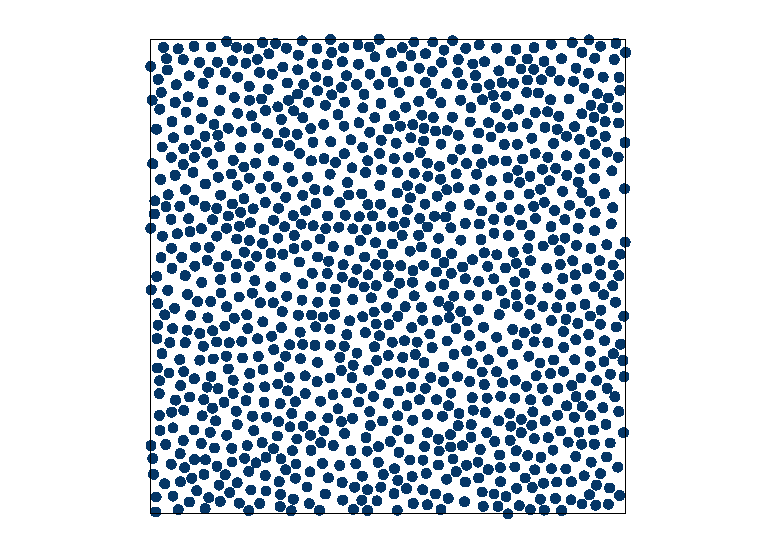
\includegraphics[width={360.00bp},height={252.00bp}]{./gnuplot/porazdelitev_1024}}%
    \gplfronttext
  \end{picture}%
\endgroup
}
    \caption[Blue noise]{Porazdelitev $1024$ točk.}
    \label{fig:porazdelitev_tock}
\end{figure}

\section{Eliptična kontaktna funkcija}
Za zaznavanje prekrivanja para elips implementiramo kontaktno funkcijo, povzeto
po~\cite{perram1985}.

\subsection{Ena elipsa}
Elipsa $A$ je definirana s~centrom $\vec{r}_A$, orientacijo $\theta_A$ in pozitivno 
definitno kvadratično formo $\mathbf{A}$ kot množica točk, za katero velja
\begin{equation}
    E_A (\vec{r}-\vec{r}_A, \theta_A) = 
    (\vec{r} - \vec{r}_A)^{\top} \mathbf{A}^{-1} (\vec{r} - \vec{r}_A)
    \begin{cases}
        \quad <1 & \text{znotraj A},\\
        \quad =1 & \text{na površini A},\\
        \quad >1 & \text{zunaj A}.
    \end{cases}
    \label{eq:elipsa}
\end{equation}
Z~uporabo rotacijske matrike $R(\theta)$ lahko $\mathbf{A}$ zapišemo kot
\begin{equation}
    \mathbf{A} (\theta_A) = \mathbf{R}(\theta_A) \hat{\mathbf{A}} 
                            \mathbf{R}^{\top}(\theta_A).
\end{equation}
Kjer je $\hat{\mathbf{A}}$ določena z~velikostjo polosi elipse $a_1$ in $a_2$ 
ter enotskih vektorjev $\vec{e}_i$ 
\begin{equation}
    \hat{\mathbf{A}} = \sum_{i=1}^{2} a_i^2 \vec{e}_i \vec{e}_i^{\top}.
\end{equation}

\subsection{Prekrivanje dveh elips}
Definiramo funkcijo
\begin{equation}
    F(\vec{r}, \lambda) = \lambda E_A (\vec{r}) + (1 - \lambda) E_B (\vec{r}),
    \label{eq:F}
\end{equation}
kot vsoto dveh elips $A$ in $B$, ter izbranega parametra $\lambda$. Tega omejimo na
interval $[0,1]$ tako, da je $F(\vec{r}, \lambda) \geq 0$. Pri fiksni vrednosti 
$\lambda$ ima $F(\vec{r}, \lambda)$ enolični minimum. 
Za skrajni vrednosti lahko trivialno zaključimo, da je minimum $F=0$ pri 
$\vec{r} = \vec{r}_B$ za $\lambda=0$ oziroma pri $\vec{r} = \vec{r}_A$ za 
$\lambda=1$. 
Za vse vmesne vrednosti $\lambda$ lego minimuma $\vec{r}$ dobimo z~minimizacijo.
Sledi
\begin{equation}
    \nabla F(\vec{r}, \lambda) = 0,
\end{equation}
oziroma
\begin{equation}
    \lambda \mathbf{A}^{-1} (\vec{r} - \vec{r}_A) + (1-\lambda) \mathbf{B}^{-1}
    (\vec{r} - \vec{r}_B) = 0.
    \label{eq:min_F}
\end{equation}
Rešitev minimizacije je pot $\vec{r}(\lambda)$ med centroma elips, ki jo lahko izrazimo 
iz enačbe~\ref{eq:min_F} kot sistem
\begin{align}
    \vec{r}(\lambda) &- \vec{r}_A = (1-\lambda) \mathbf{A} \mathbf{C}^{-1} 
        \vec{r}_{A B}, \nonumber \\
    \vec{r}(\lambda) &- \vec{r}_B = - \lambda \mathbf{B} \mathbf{C}^{-1} \vec{r}_{A B}, 
    \label{eq:rab}
\end{align}
kjer sta $\vec{r}_{A B} = \vec{r}_B - \vec{r}_A$ in $\mathbf{C}$ vsota
\begin{equation}
    \mathbf{C} = (1-\lambda) \mathbf{A} + \lambda \mathbf{B}.
    \label{eq:C}
\end{equation}
saj sta matriki $\mathbf{A}$ in $\mathbf{B}$ pozitivno 
definitni.
Rešitev~\ref{eq:rab} uporabimo v~enačbi~\ref{eq:F}, pri čemer upoštevamo tudi
enačbo~\ref{eq:C} in definiramo funkcijo $f$, ki ni več eksplicitno odvisna od 
$\vec{r}(\lambda)$
\begin{equation}
    f(\lambda) = F (\vec{r}(\lambda), \lambda) = \lambda (1-\lambda)
        \vec{r}_{A B}^{\top} \mathbf{C}^{-1} \vec{r}_{A B}.
\end{equation}
\begin{figure}[!ht]
    \centering
    \resizebox{.5\textwidth}{!}{\begin{tikzpicture}

\pgfmathsetmacro{\as}{1.5};
\pgfmathsetmacro{\bs}{0.5};
\pgfmathsetmacro{\cs}{sqrt(\as^2 - \bs^2)}
\pgfmathsetmacro{\al}{1.5};
\pgfmathsetmacro{\bl}{1};
\pgfmathsetmacro{\cl}{sqrt(\al^2 - \bl^2)}
\pgfmathsetmacro{\xs}{abs(\cs - \cl)}


\draw (0, 0) ellipse [x radius = \as cm, y radius = \bs cm] node[above, scale=0.8] {$\vec{r}_a$};
\draw [rotate around={-45:(1, 1.5)}] (1,1.5) ellipse [x radius = \al cm, y radius = \bl cm] node[above, scale=0.8] {$\vec{r}_b$};

\begin{axis}[
    anchor=origin,
    x=1cm, y=1cm,
    no marks,
    clip=false,
    axis line style={draw=none},
    tick style={draw=none},
    yticklabels={,,},
    xticklabels={,,},
    ]
    % this parametric plot was calculated with mathematica
    \addplot [domain=0:1,samples=100,mygreen,thick]({(33.75*(1 - x)*x)/(9 + 47*x - 20*x^2) + ( 9*(1 - x) * (1 + (11*x)/2))/(9 + 47*x - 20*x^2)}, {5*(1 - x)*x/(2 * (9 + 47*x - 20*x^2)) + ( 1.5*(1 - x) * (9 * (1 - x) + 13 *x /2))/(9 + 47*x- 20*x^2});

\end{axis}

\node[scale=0.8] at (1.5,0.5) {$\vec{r}(\lambda )$};

\filldraw[black] (0, 0) circle [radius = 0.01 cm];
\filldraw[black] (1, 1.5) circle [radius = 0.01 cm];

\node[scale=0.8] at (-0.5,0.7) {$A$};
\node[scale=0.8] at (-0.5,2) {$B$};

\end{tikzpicture}
% 33.75*(1 - x)*x/(9 + 47*x - 20*x^2) + ( 9*(1 - x) * (1 + (11*x)/2))/(9 + 47*x - 20*x^2)
% 5*(1 - x)*x/(2 * (9 + 47*x - 20*x^2)) + ( 1.5*(1 - x) * (9 * (1 - x) + 13 *x /2))/(9 + 47*x- 20*x^2)}
    \caption{Minimalna pot $\vec{r}(\lambda)$ gre skozi presek elips $A$ in $B$.}
    \label{fig:path}
\end{figure}\\
\noindent Poglejmo kako se obnaša pot $\vec{r}(\lambda), \, \lambda \in [0,1]$, ki povezuje 
centra elips med seboj -- kar lahko vidimo na sliki~\ref{fig:path}.
Iz enačbe~\ref{eq:elipsa} sledi, da je vrednost $F(\vec{r}, \lambda)$ na območju 
izven obeh elips $F(\vec{r}, \lambda)>1$. Če se $A$ in $B$ ne sekata, potem mora imeti 
pot minimuma $F(\vec{r}, \lambda)>1$ vrednost večjo od $1$. Če se $A$ in $B$ prekrivata 
potem je vrednost $F(\vec{r}, \lambda)<1$ na preseku $A \cap B$ za katerokoli vrednost 
$\lambda \in [0,1]$.  Sledi, da je vrednost minimuma $F(\vec{r}, \lambda)<1$ zagotovo 
manjša od $1$. To pomeni, da pot $\vec{r}(\lambda)$ zagotovo ne bo šla izven območij
$A$ in $B$. Zaključimo, da za vrednosti $F(\vec{r}(\lambda), \lambda) = 
f(\lambda)$ velja
\begin{equation}
    \max_{0<\lambda<1} f(\lambda)
    \begin{cases}
        <1 \quad\text{$A$ in $B$ se prekrivata,}\\
        =1 \quad\text{$A$ in $B$ sta tangentni,}\\
        >1 \quad\text{$A$ in $B$ se ne dotikata.}
    \end{cases}
    \label{eq:kriterij}
\end{equation}
Te lastnosti izkoristimo pri definiciji kontaktne funkcije med dvema elipsama, tako da
velja
\begin{equation}
    F_{A B}(\vec{r}_{A B}, \theta_A, \theta_B) =
    \max_{0<\lambda<1} f(\lambda) = \mu^2.
    \label{eq:kontakt}
\end{equation}
Vrednost $\mu$ je linearni faktor s~katerim moramo množiti elipsi $A$ in $B$, da 
postaneta tangentni.
\subsection{Zaznavanje prekrivanj s~kontaktno funkcijo}
Vpeljano kontaktno funkcijo uporabimo na porazdelitvi elips, ki smo jo zgenerirali
z~Mitchellovim algoritmom. 
Za primer poglejmo sliko~\ref{fig:zaznavanje_trkov}, ki prikazuje porazdelitev
$128$ elips. Izberemo naključno elipso in pogledamo njeno okolico polmera $2a$.
S~tem zmanjšamo število parov elips na katerih moramo računati kontaktno funkcijo.
\begin{figure}[!ht]
    \centering
    \resizebox{.32\textwidth}{!}{% This file was created with tikzplotlib v0.10.1.
\begin{tikzpicture}

\definecolor{darkgray176}{RGB}{176,176,176}
\definecolor{steelblue31119180}{RGB}{31,119,180}

\begin{axis}[
    x=2, y=2,
    x grid style={darkgray176},
    xmin=0, xmax=100,
    y grid style={darkgray176},
    ymin=0, ymax=100,
    tick style={draw=none},
    yticklabels={,,},
    xtick
]
\draw[draw=none,fill=myblue,rotate around={260.204650150668:(axis cs:86.882913846962,41.6777189680256)}] (axis cs:86.882913846962,41.6777189680256) ellipse (5 and 2);
\draw[draw=none,fill=myblue,rotate around={352.916970683532:(axis cs:17.3702053810315,60.1099457262999)}] (axis cs:17.3702053810315,60.1099457262999) ellipse (5 and 2);
\draw[draw=none,fill=myblue,rotate around={22.6137910135262:(axis cs:54.3578505168292,28.8121800265779)}] (axis cs:54.3578505168292,28.8121800265779) ellipse (5 and 2);
\draw[draw=none,fill=myblue,rotate around={54.1605172415885:(axis cs:26.8061313592254,93.4547820902352)}] (axis cs:26.8061313592254,93.4547820902352) ellipse (5 and 2);
\draw[draw=none,fill=myblue,rotate around={349.787045848476:(axis cs:92.8377033572501,97.06536507931)}] (axis cs:92.8377033572501,97.06536507931) ellipse (5 and 2);
\draw[draw=none,fill=myblue,rotate around={301.169459612978:(axis cs:28.7329585023873,31.0188006699616)}] (axis cs:28.7329585023873,31.0188006699616) ellipse (5 and 2);
\draw[draw=none,fill=myblue,rotate around={9.99665572168897:(axis cs:64.8146228143106,1.40202864166694)}] (axis cs:64.8146228143106,1.40202864166694) ellipse (5 and 2);
\draw[draw=none,fill=myblue,rotate around={75.9590718992238:(axis cs:48.3915146177629,64.1181420805372)}] (axis cs:48.3915146177629,64.1181420805372) ellipse (5 and 2);
\draw[draw=none,fill=myblue,rotate around={227.038747519095:(axis cs:81.3272540913949,17.500793155944)}] (axis cs:81.3272540913949,17.500793155944) ellipse (5 and 2);
\draw[draw=none,fill=myblue,rotate around={248.168331406681:(axis cs:99.3939573851162,14.3982292725168)}] (axis cs:99.3939573851162,14.3982292725168) ellipse (5 and 2);
\draw[draw=none,fill=myblue,rotate around={190.315288515932:(axis cs:75.6429101109758,76.6325837014612)}] (axis cs:75.6429101109758,76.6325837014612) ellipse (5 and 2);
\draw[draw=none,fill=myblue,rotate around={52.992867030674:(axis cs:4.98633355030644,55.0858130674453)}] (axis cs:4.98633355030644,55.0858130674453) ellipse (5 and 2);
\draw[draw=none,fill=myblue,rotate around={54.0037365377994:(axis cs:39.5055460595019,39.9625444177252)}] (axis cs:39.5055460595019,39.9625444177252) ellipse (5 and 2);
\draw[draw=none,fill=myblue,rotate around={332.863827568311:(axis cs:71.3013949179524,43.9153887693566)}] (axis cs:71.3013949179524,43.9153887693566) ellipse (5 and 2);
\draw[draw=none,fill=myblue,rotate around={84.5473125880316:(axis cs:1.86286810442203,76.1448652422809)}] (axis cs:1.86286810442203,76.1448652422809) ellipse (5 and 2);
\draw[draw=none,fill=myblue,rotate around={294.754598975761:(axis cs:40.2510821396431,3.23948125486693)}] (axis cs:40.2510821396431,3.23948125486693) ellipse (5 and 2);
\draw[draw=none,fill=myblue,rotate around={353.860974913289:(axis cs:32.2412530863386,66.6502536503754)}] (axis cs:32.2412530863386,66.6502536503754) ellipse (5 and 2);
\draw[draw=none,fill=myblue,rotate around={268.079369117024:(axis cs:87.8331224981219,55.6504236167273)}] (axis cs:87.8331224981219,55.6504236167273) ellipse (5 and 2);
\draw[draw=none,fill=myblue,rotate around={249.914628955572:(axis cs:40.4644776697715,88.6819898491135)}] (axis cs:40.4644776697715,88.6819898491135) ellipse (5 and 2);
\draw[draw=none,fill=myblue,rotate around={315.9419617351:(axis cs:2.21483365114915,39.0946442609324)}] (axis cs:2.21483365114915,39.0946442609324) ellipse (5 and 2);
\draw[draw=none,fill=myblue,rotate around={29.7482081236702:(axis cs:12.948532403687,20.3052301632043)}] (axis cs:12.948532403687,20.3052301632043) ellipse (5 and 2);
\draw[draw=none,fill=myblue,rotate around={245.9296477557:(axis cs:9.21255957094804,2.22727254610813)}] (axis cs:9.21255957094804,2.22727254610813) ellipse (5 and 2);
\draw[draw=none,fill=myblue,rotate around={10.5803347867585:(axis cs:56.7525384036258,14.9822704642782)}] (axis cs:56.7525384036258,14.9822704642782) ellipse (5 and 2);
\draw[draw=none,fill=myblue,rotate around={231.67969665037:(axis cs:94.6296514046673,27.5593228059429)}] (axis cs:94.6296514046673,27.5593228059429) ellipse (5 and 2);
\draw[draw=none,fill=myblue,rotate around={246.320529683567:(axis cs:40.2988588854947,24.6222243618935)}] (axis cs:40.2988588854947,24.6222243618935) ellipse (5 and 2);
\draw[draw=none,fill=myblue,rotate around={345.812285412304:(axis cs:89.1671087210519,78.1531769002003)}] (axis cs:89.1671087210519,78.1531769002003) ellipse (5 and 2);
\draw[draw=none,fill=myblue,rotate around={319.270432431842:(axis cs:57.9576260069661,51.5378189312098)}] (axis cs:57.9576260069661,51.5378189312098) ellipse (5 and 2);
\draw[draw=none,fill=myblue,rotate around={98.5717374651543:(axis cs:20.7427655078686,44.4798361153012)}] (axis cs:20.7427655078686,44.4798361153012) ellipse (5 and 2);
\draw[draw=none,fill=myblue,rotate around={320.301578164404:(axis cs:2.81441707119023,90.2466579598913)}] (axis cs:2.81441707119023,90.2466579598913) ellipse (5 and 2);
\draw[draw=none,fill=myblue,rotate around={76.4647671337003:(axis cs:76.0905857450005,94.3357690743821)}] (axis cs:76.0905857450005,94.3357690743821) ellipse (5 and 2);
\draw[draw=none,fill=myblue,rotate around={84.9272953979372:(axis cs:11.9019594584809,81.9433638347379)}] (axis cs:11.9019594584809,81.9433638347379) ellipse (5 and 2);
\draw[draw=none,fill=myblue,rotate around={204.607367274743:(axis cs:79.8625822264079,65.311187764344)}] (axis cs:79.8625822264079,65.311187764344) ellipse (5 and 2);
\draw[draw=none,fill=myblue,rotate around={12.3739793687086:(axis cs:21.323586325317,71.8427228400097)}] (axis cs:21.323586325317,71.8427228400097) ellipse (5 and 2);
\draw[draw=none,fill=myblue,rotate around={117.168001814191:(axis cs:26.195767740668,16.3937377096593)}] (axis cs:26.195767740668,16.3937377096593) ellipse (5 and 2);
\draw[draw=none,fill=myblue,rotate around={274.460391494636:(axis cs:39.6281320324819,54.8484672789167)}] (axis cs:39.6281320324819,54.8484672789167) ellipse (5 and 2);
\draw[draw=none,fill=myblue,rotate around={130.54913502052:(axis cs:55.933435835093,79.8429238370018)}] (axis cs:55.933435835093,79.8429238370018) ellipse (5 and 2);
\draw[draw=none,fill=myblue,rotate around={132.433882308199:(axis cs:50.9653840442826,91.1428552378015)}] (axis cs:50.9653840442826,91.1428552378015) ellipse (5 and 2);
\draw[draw=none,fill=myblue,rotate around={69.0335688009109:(axis cs:63.3896028126425,63.0007610550364)}] (axis cs:63.3896028126425,63.0007610550364) ellipse (5 and 2);
\draw[draw=none,fill=myblue,rotate around={3.85375435108094:(axis cs:18.6121409896952,6.44416862770173)}] (axis cs:18.6121409896952,6.44416862770173) ellipse (5 and 2);
\draw[draw=none,fill=myblue,rotate around={242.14725970489:(axis cs:68.1720522704402,88.0252489706398)}] (axis cs:68.1720522704402,88.0252489706398) ellipse (5 and 2);
\draw[draw=none,fill=myblue,rotate around={289.801943190306:(axis cs:43.1108191914449,74.7060050602938)}] (axis cs:43.1108191914449,74.7060050602938) ellipse (5 and 2);
\draw[draw=none,fill=myblue,rotate around={282.464320644406:(axis cs:69.9923435700512,15.6729689301564)}] (axis cs:69.9923435700512,15.6729689301564) ellipse (5 and 2);
\draw[draw=none,fill=myblue,rotate around={234.724822456551:(axis cs:1.89041207297357,63.8556494308399)}] (axis cs:1.89041207297357,63.8556494308399) ellipse (5 and 2);
\draw[draw=none,fill=myblue,rotate around={302.616093260557:(axis cs:19.772606026042,30.5471205146096)}] (axis cs:19.772606026042,30.5471205146096) ellipse (5 and 2);
\draw[draw=none,fill=myblue,rotate around={158.340760048643:(axis cs:47.7631607343279,6.91010886104096)}] (axis cs:47.7631607343279,6.91010886104096) ellipse (5 and 2);
\draw[draw=none,fill=myblue,rotate around={202.054523659658:(axis cs:71.7026363458189,24.2772963730362)}] (axis cs:71.7026363458189,24.2772963730362) ellipse (5 and 2);
\draw[draw=none,fill=myblue,rotate around={69.6380570029668:(axis cs:15.5768836156765,93.8502782854917)}] (axis cs:15.5768836156765,93.8502782854917) ellipse (5 and 2);
\draw[draw=none,fill=myblue,rotate around={152.575999415476:(axis cs:88.8183765619847,68.9473725156417)}] (axis cs:88.8183765619847,68.9473725156417) ellipse (5 and 2);
\draw[draw=none,fill=myblue,rotate around={86.6229821231618:(axis cs:81.5765245617972,5.2010753658165)}] (axis cs:81.5765245617972,5.2010753658165) ellipse (5 and 2);
\draw[draw=none,fill=myblue,rotate around={69.5870529278177:(axis cs:65.8506228342984,33.3603805241784)}] (axis cs:65.8506228342984,33.3603805241784) ellipse (5 and 2);
\draw[draw=none,fill=myblue,rotate around={89.4563598649543:(axis cs:28.4867819268627,51.8325293958749)}] (axis cs:28.4867819268627,51.8325293958749) ellipse (5 and 2);
\draw[draw=none,fill=myblue,rotate around={118.92867917955:(axis cs:37.1783840900199,15.0048162820745)}] (axis cs:37.1783840900199,15.0048162820745) ellipse (5 and 2);
\draw[draw=none,fill=myblue,rotate around={10.7885285332415:(axis cs:91.2306043988741,9.00705471851809)}] (axis cs:91.2306043988741,9.00705471851809) ellipse (5 and 2);
\draw[draw=none,fill=myblue,rotate around={70.766031758227:(axis cs:83.3116224870324,26.9941651840805)}] (axis cs:83.3116224870324,26.9941651840805) ellipse (5 and 2);
\draw[draw=none,fill=myblue,rotate around={35.6434088614135:(axis cs:68.8597459043663,54.9424041219192)}] (axis cs:68.8597459043663,54.9424041219192) ellipse (5 and 2);
\draw[draw=none,fill=myblue,rotate around={51.5476613473339:(axis cs:27.6855305634842,7.33028459895518)}] (axis cs:27.6855305634842,7.33028459895518) ellipse (5 and 2);
\draw[draw=none,fill=myblue,rotate around={346.299933178858:(axis cs:48.2056048404719,39.6634016751004)}] (axis cs:48.2056048404719,39.6634016751004) ellipse (5 and 2);
\draw[draw=none,fill=myblue,rotate around={265.618518135428:(axis cs:30.5569873761105,79.5161765830348)}] (axis cs:30.5569873761105,79.5161765830348) ellipse (5 and 2);
\draw[draw=none,fill=myblue,rotate around={103.45201055566:(axis cs:58.9588736685684,89.1863749433072)}] (axis cs:58.9588736685684,89.1863749433072) ellipse (5 and 2);
\draw[draw=none,fill=myblue,rotate around={220.502650942834:(axis cs:60.5080407877913,41.8210802578143)}] (axis cs:60.5080407877913,41.8210802578143) ellipse (5 and 2);
\draw[draw=none,fill=myblue,rotate around={218.80828811829:(axis cs:55.7205303388384,67.860496152752)}] (axis cs:55.7205303388384,67.860496152752) ellipse (5 and 2);
\draw[draw=none,fill=myblue,rotate around={150.520494903969:(axis cs:56.2460532738079,99.98891155317)}] (axis cs:56.2460532738079,99.98891155317) ellipse (5 and 2);
\draw[draw=none,fill=myblue,rotate around={54.8255110517293:(axis cs:92.5194453046932,86.236230748634)}] (axis cs:92.5194453046932,86.236230748634) ellipse (5 and 2);
\draw[draw=none,fill=myblue,rotate around={300.366524500867:(axis cs:5.04996349555212,30.2011265445795)}] (axis cs:5.04996349555212,30.2011265445795) ellipse (5 and 2);
\draw[draw=none,fill=myblue,rotate around={254.060351773917:(axis cs:7.53779290855019,10.5024775779718)}] (axis cs:7.53779290855019,10.5024775779718) ellipse (5 and 2);
\draw[draw=none,fill=myblue,rotate around={294.878692522367:(axis cs:65.7557552355382,72.5896944885608)}] (axis cs:65.7557552355382,72.5896944885608) ellipse (5 and 2);
\draw[draw=none,fill=myblue,rotate around={16.7930611338574:(axis cs:12.7640613253374,72.239375523327)}] (axis cs:12.7640613253374,72.239375523327) ellipse (5 and 2);
\draw[draw=none,fill=myblue,rotate around={86.396868066909:(axis cs:10.0538312195155,38.1153271806579)}] (axis cs:10.0538312195155,38.1153271806579) ellipse (5 and 2);
\draw[draw=none,fill=myblue,rotate around={324.027291154328:(axis cs:49.0019491046676,52.1085809997291)}] (axis cs:49.0019491046676,52.1085809997291) ellipse (5 and 2);
\draw[draw=none,fill=myblue,rotate around={67.9654909980869:(axis cs:94.255974386524,36.5108506935766)}] (axis cs:94.255974386524,36.5108506935766) ellipse (5 and 2);
\draw[draw=none,fill=myblue,rotate around={251.941321158686:(axis cs:12.763648487112,45.4459238854269)}] (axis cs:12.763648487112,45.4459238854269) ellipse (5 and 2);
\draw[draw=none,fill=myblue,rotate around={190.351190759998:(axis cs:48.833234251249,20.9506374190798)}] (axis cs:48.833234251249,20.9506374190798) ellipse (5 and 2);
\draw[draw=none,fill=myblue,rotate around={298.612113224356:(axis cs:22.8495523863503,82.5045499767124)}] (axis cs:22.8495523863503,82.5045499767124) ellipse (5 and 2);
\draw[draw=none,fill=myblue,rotate around={352.400434801704:(axis cs:96.1055748110164,45.0288993232664)}] (axis cs:96.1055748110164,45.0288993232664) ellipse (5 and 2);
\draw[draw=none,fill=myblue,rotate around={24.9758141740133:(axis cs:71.1141108281389,6.83262257865851)}] (axis cs:71.1141108281389,6.83262257865851) ellipse (5 and 2);
\draw[draw=none,fill=myblue,rotate around={47.1120904509369:(axis cs:35.4257600506402,47.9798120950139)}] (axis cs:35.4257600506402,47.9798120950139) ellipse (5 and 2);
\draw[draw=none,fill=myblue,rotate around={14.7746567560795:(axis cs:81.0140107259634,48.6829084944324)}] (axis cs:81.0140107259634,48.6829084944324) ellipse (5 and 2);
\draw[draw=none,fill=myblue,rotate around={307.896545207601:(axis cs:84.0823937105312,83.8764630495301)}] (axis cs:84.0823937105312,83.8764630495301) ellipse (5 and 2);
\draw[draw=none,fill=myblue,rotate around={185.319571851166:(axis cs:55.6619378201471,58.8078579678459)}] (axis cs:55.6619378201471,58.8078579678459) ellipse (5 and 2);
\draw[draw=none,fill=myblue,rotate around={325.172336062301:(axis cs:41.4907403776405,32.3506445488188)}] (axis cs:41.4907403776405,32.3506445488188) ellipse (5 and 2);
\draw[draw=none,fill=myblue,rotate around={119.872128201725:(axis cs:89.6719005334523,18.9791507390857)}] (axis cs:89.6719005334523,18.9791507390857) ellipse (5 and 2);
\draw[draw=none,fill=myblue,rotate around={357.821530747641:(axis cs:9.62782038925507,62.1232922938803)}] (axis cs:9.62782038925507,62.1232922938803) ellipse (5 and 2);
\draw[draw=none,fill=myblue,rotate around={326.408690547729:(axis cs:85.9872570382636,93.5585714150404)}] (axis cs:85.9872570382636,93.5585714150404) ellipse (5 and 2);
\draw[draw=none,fill=myblue,rotate around={165.491621211313:(axis cs:63.768546413739,22.5593396318724)}] (axis cs:63.768546413739,22.5593396318724) ellipse (5 and 2);
\draw[draw=none,fill=myblue,rotate around={62.5689723853916:(axis cs:45.999869632787,81.9718303639362)}] (axis cs:45.999869632787,81.9718303639362) ellipse (5 and 2);
\draw[draw=none,fill=myblue,rotate around={80.686868301937:(axis cs:40.513972119891,63.2574647102097)}] (axis cs:40.513972119891,63.2574647102097) ellipse (5 and 2);
\draw[draw=none,fill=myblue,rotate around={352.160175168487:(axis cs:0.670179449571862,1.8587023245636)}] (axis cs:0.670179449571862,1.8587023245636) ellipse (5 and 2);
\draw[draw=none,fill=myblue,rotate around={147.152087004351:(axis cs:74.5059127687272,32.94117457168)}] (axis cs:74.5059127687272,32.94117457168) ellipse (5 and 2);
\draw[draw=none,fill=myblue,rotate around={79.912177589682:(axis cs:99.5409900854364,83.3507452903862)}] (axis cs:99.5409900854364,83.3507452903862) ellipse (5 and 2);
\draw[draw=none,fill=myblue,rotate around={0.893218153011031:(axis cs:30.6413648667477,39.4308194959482)}] (axis cs:30.6413648667477,39.4308194959482) ellipse (5 and 2);
\draw[draw=none,fill=myblue,rotate around={149.39430802483:(axis cs:16.364079445829,13.1332597438818)}] (axis cs:16.364079445829,13.1332597438818) ellipse (5 and 2);
\draw[draw=none,fill=myblue,rotate around={263.614140785283:(axis cs:81.4779667377777,59.1129447486611)}] (axis cs:81.4779667377777,59.1129447486611) ellipse (5 and 2);
\draw[draw=none,fill=myblue,rotate around={356.776002302174:(axis cs:1.58847438749508,22.0501701614518)}] (axis cs:1.58847438749508,22.0501701614518) ellipse (5 and 2);
\draw[draw=none,fill=myblue,rotate around={170.091144245238:(axis cs:31.0423654417477,99.2149038897966)}] (axis cs:31.0423654417477,99.2149038897966) ellipse (5 and 2);
\draw[draw=none,fill=myblue,rotate around={130.754835632223:(axis cs:46.9468771825903,98.6594198824206)}] (axis cs:46.9468771825903,98.6594198824206) ellipse (5 and 2);
\draw[draw=none,fill=myblue,rotate around={177.160830537073:(axis cs:74.2938016624452,50.2051842249504)}] (axis cs:74.2938016624452,50.2051842249504) ellipse (5 and 2);
\draw[draw=none,fill=myblue,rotate around={242.728282134562:(axis cs:78.6279318778352,38.5714724755397)}] (axis cs:78.6279318778352,38.5714724755397) ellipse (5 and 2);
\draw[draw=none,fill=myblue,rotate around={92.6718119634767:(axis cs:9.83995614919241,88.6061914819749)}] (axis cs:9.83995614919241,88.6061914819749) ellipse (5 and 2);
\draw[draw=none,fill=myblue,rotate around={154.348461856241:(axis cs:94.6984370754419,52.6195822773216)}] (axis cs:94.6984370754419,52.6195822773216) ellipse (5 and 2);
\draw[draw=none,fill=myblue,rotate around={163.428804825857:(axis cs:12.3813878424189,53.7827644674075)}] (axis cs:12.3813878424189,53.7827644674075) ellipse (5 and 2);
\draw[draw=none,fill=myblue,rotate around={242.708068430962:(axis cs:27.8300822695283,58.8917633929874)}] (axis cs:27.8300822695283,58.8917633929874) ellipse (5 and 2);
\draw[draw=none,fill=myblue,rotate around={235.475628484884:(axis cs:96.2473706632951,70.984470876944)}] (axis cs:96.2473706632951,70.984470876944) ellipse (5 and 2);
\draw[draw=none,fill=myblue,rotate around={36.656268675175:(axis cs:31.8306870443883,87.8458564448473)}] (axis cs:31.8306870443883,87.8458564448473) ellipse (5 and 2);
\draw[draw=none,fill=myblue,rotate around={112.043249573373:(axis cs:63.7252837899546,94.8004298199742)}] (axis cs:63.7252837899546,94.8004298199742) ellipse (5 and 2);
\draw[draw=none,fill=myblue,rotate around={92.0523885815362:(axis cs:53.4661151748034,45.9549267427767)}] (axis cs:53.4661151748034,45.9549267427767) ellipse (5 and 2);
\draw[draw=none,fill=myblue,rotate around={245.449379453127:(axis cs:55.0511046066284,36.2202640673709)}] (axis cs:55.0511046066284,36.2202640673709) ellipse (5 and 2);
\draw[draw=none,fill=myblue,rotate around={295.652389779659:(axis cs:85.8883818155678,34.0384614709201)}] (axis cs:85.8883818155678,34.0384614709201) ellipse (5 and 2);
\draw[draw=none,fill=myblue,rotate around={225.194198562187:(axis cs:64.0823849056176,81.0403814957276)}] (axis cs:64.0823849056176,81.0403814957276) ellipse (5 and 2);
\draw[draw=none,fill=myblue,rotate around={96.995820274412:(axis cs:51.3744048894096,73.8743045476509)}] (axis cs:51.3744048894096,73.8743045476509) ellipse (5 and 2);
\draw[draw=none,fill=myblue,rotate around={98.0898695872326:(axis cs:21.8022369733386,22.7350748099463)}] (axis cs:21.8022369733386,22.7350748099463) ellipse (5 and 2);
\draw[draw=none,fill=myblue,rotate around={138.78854758218:(axis cs:31.6959886698282,22.3058845988067)}] (axis cs:31.6959886698282,22.3058845988067) ellipse (5 and 2);
\draw[draw=none,fill=myblue,rotate around={318.492823597775:(axis cs:95.5877271140043,61.8264497134761)}] (axis cs:95.5877271140043,61.8264497134761) ellipse (5 and 2);
\draw[draw=none,fill=myblue,rotate around={259.231220358722:(axis cs:21.4771599692152,99.5192993241954)}] (axis cs:21.4771599692152,99.5192993241954) ellipse (5 and 2);
\draw[draw=none,fill=myblue,rotate around={269.741531872192:(axis cs:3.25648736233763,47.5197410511917)}] (axis cs:3.25648736233763,47.5197410511917) ellipse (5 and 2);
\draw[draw=none,fill=myblue,rotate around={297.353285854387:(axis cs:61.218038462067,8.28676729492537)}] (axis cs:61.218038462067,8.28676729492537) ellipse (5 and 2);
\draw[draw=none,fill=myblue,rotate around={47.726999713751:(axis cs:23.780568342442,36.0723097613012)}] (axis cs:23.780568342442,36.0723097613012) ellipse (5 and 2);
\draw[draw=none,fill=myblue,rotate around={77.7238081358585:(axis cs:83.1646923435251,11.4032470035099)}] (axis cs:83.1646923435251,11.4032470035099) ellipse (5 and 2);
\draw[draw=none,fill=myblue,rotate around={317.080766857636:(axis cs:72.4044215935182,63.3080070150894)}] (axis cs:72.4044215935182,63.3080070150894) ellipse (5 and 2);
\draw[draw=none,fill=myblue,rotate around={38.7891838094475:(axis cs:12.5489499377054,29.7759902549972)}] (axis cs:12.5489499377054,29.7759902549972) ellipse (5 and 2);
\draw[draw=none,fill=myblue,rotate around={313.711203512664:(axis cs:89.5227528142594,47.8325968256834)}] (axis cs:89.5227528142594,47.8325968256834) ellipse (5 and 2);
\draw[draw=none,fill=myblue,rotate around={298.477328346312:(axis cs:72.9707250021413,99.7706074619335)}] (axis cs:72.9707250021413,99.7706074619335) ellipse (5 and 2);
\draw[draw=none,fill=myblue,rotate around={5.81423179660655:(axis cs:22.6543381808917,54.6284359265346)}] (axis cs:22.6543381808917,54.6284359265346) ellipse (5 and 2);
\draw[draw=none,fill=myblue,rotate around={107.369343119315:(axis cs:76.8084025367909,11.622625330049)}] (axis cs:76.8084025367909,11.622625330049) ellipse (5 and 2);
\draw[draw=none,fill=myblue,rotate around={297.410687409085:(axis cs:82.316163382063,77.0255989351747)}] (axis cs:82.316163382063,77.0255989351747) ellipse (5 and 2);
\draw[draw=none,fill=myblue,rotate around={241.412768220482:(axis cs:95.6908177165746,77.8990008145085)}] (axis cs:95.6908177165746,77.8990008145085) ellipse (5 and 2);
\draw[draw=none,fill=myblue,rotate around={306.721684207499:(axis cs:46.0121623420069,57.6240632220017)}] (axis cs:46.0121623420069,57.6240632220017) ellipse (5 and 2);
\draw[draw=none,fill=myblue,rotate around={322.736476985811:(axis cs:27.1112894933776,73.6073827622796)}] (axis cs:27.1112894933776,73.6073827622796) ellipse (5 and 2);
\draw[draw=none,fill=myblue,rotate around={77.4649729853431:(axis cs:77.8123782915191,87.7467385017039)}] (axis cs:77.8123782915191,87.7467385017039) ellipse (5 and 2);
\end{axis}

\end{tikzpicture}
}
    \resizebox{.32\textwidth}{!}{% This file was created with tikzplotlib v0.10.1.
\begin{tikzpicture}

\definecolor{darkgray176}{RGB}{176,176,176}
\definecolor{gray}{RGB}{128,128,128}
\definecolor{steelblue31119180}{RGB}{31,119,180}

\begin{axis}[
    x=2, y=2,
    x grid style={darkgray176},
    xmin=0, xmax=100,
    y grid style={darkgray176},
    ymin=0, ymax=100,
    tick style={draw=none},
    yticklabels={,,},
    xtick
]
\draw[draw=none,fill=myblue,rotate around={260.204650150668:(axis cs:86.882913846962,41.6777189680256)}] (axis cs:86.882913846962,41.6777189680256) ellipse (5 and 2);
\draw[draw=none,fill=myblue,rotate around={352.916970683532:(axis cs:17.3702053810315,60.1099457262999)}] (axis cs:17.3702053810315,60.1099457262999) ellipse (5 and 2);
\draw[draw=none,fill=myblue,rotate around={22.6137910135262:(axis cs:54.3578505168292,28.8121800265779)}] (axis cs:54.3578505168292,28.8121800265779) ellipse (5 and 2);
\draw[draw=none,fill=myblue,rotate around={54.1605172415885:(axis cs:26.8061313592254,93.4547820902352)}] (axis cs:26.8061313592254,93.4547820902352) ellipse (5 and 2);
\draw[draw=none,fill=myblue,rotate around={349.787045848476:(axis cs:92.8377033572501,97.06536507931)}] (axis cs:92.8377033572501,97.06536507931) ellipse (5 and 2);
\draw[draw=none,fill=myblue,rotate around={301.169459612978:(axis cs:28.7329585023873,31.0188006699616)}] (axis cs:28.7329585023873,31.0188006699616) ellipse (5 and 2);
\draw[draw=none,fill=myblue,rotate around={9.99665572168897:(axis cs:64.8146228143106,1.40202864166694)}] (axis cs:64.8146228143106,1.40202864166694) ellipse (5 and 2);
\draw[draw=none,fill=myblue,rotate around={75.9590718992238:(axis cs:48.3915146177629,64.1181420805372)}] (axis cs:48.3915146177629,64.1181420805372) ellipse (5 and 2);
\draw[draw=none,fill=myblue,rotate around={227.038747519095:(axis cs:81.3272540913949,17.500793155944)}] (axis cs:81.3272540913949,17.500793155944) ellipse (5 and 2);
\draw[draw=none,fill=myblue,rotate around={248.168331406681:(axis cs:99.3939573851162,14.3982292725168)}] (axis cs:99.3939573851162,14.3982292725168) ellipse (5 and 2);
\draw[draw=none,fill=myblue,rotate around={190.315288515932:(axis cs:75.6429101109758,76.6325837014612)}] (axis cs:75.6429101109758,76.6325837014612) ellipse (5 and 2);
\draw[draw=none,fill=myblue,rotate around={52.992867030674:(axis cs:4.98633355030644,55.0858130674453)}] (axis cs:4.98633355030644,55.0858130674453) ellipse (5 and 2);
\draw[draw=none,fill=myblue,rotate around={54.0037365377994:(axis cs:39.5055460595019,39.9625444177252)}] (axis cs:39.5055460595019,39.9625444177252) ellipse (5 and 2);
\draw[draw=none,fill=myblue,rotate around={332.863827568311:(axis cs:71.3013949179524,43.9153887693566)}] (axis cs:71.3013949179524,43.9153887693566) ellipse (5 and 2);
\draw[draw=none,fill=myblue,rotate around={84.5473125880316:(axis cs:1.86286810442203,76.1448652422809)}] (axis cs:1.86286810442203,76.1448652422809) ellipse (5 and 2);
\draw[draw=none,fill=myblue,rotate around={294.754598975761:(axis cs:40.2510821396431,3.23948125486693)}] (axis cs:40.2510821396431,3.23948125486693) ellipse (5 and 2);
\draw[draw=none,fill=myblue,rotate around={353.860974913289:(axis cs:32.2412530863386,66.6502536503754)}] (axis cs:32.2412530863386,66.6502536503754) ellipse (5 and 2);
\draw[draw=none,fill=myblue,rotate around={268.079369117024:(axis cs:87.8331224981219,55.6504236167273)}] (axis cs:87.8331224981219,55.6504236167273) ellipse (5 and 2);
\draw[draw=none,fill=myblue,rotate around={249.914628955572:(axis cs:40.4644776697715,88.6819898491135)}] (axis cs:40.4644776697715,88.6819898491135) ellipse (5 and 2);
\draw[draw=none,fill=myblue,rotate around={315.9419617351:(axis cs:2.21483365114915,39.0946442609324)}] (axis cs:2.21483365114915,39.0946442609324) ellipse (5 and 2);
\draw[draw=none,fill=myblue,rotate around={29.7482081236702:(axis cs:12.948532403687,20.3052301632043)}] (axis cs:12.948532403687,20.3052301632043) ellipse (5 and 2);
\draw[draw=none,fill=myblue,rotate around={245.9296477557:(axis cs:9.21255957094804,2.22727254610813)}] (axis cs:9.21255957094804,2.22727254610813) ellipse (5 and 2);
\draw[draw=none,fill=myblue,rotate around={10.5803347867585:(axis cs:56.7525384036258,14.9822704642782)}] (axis cs:56.7525384036258,14.9822704642782) ellipse (5 and 2);
\draw[draw=none,fill=myblue,rotate around={231.67969665037:(axis cs:94.6296514046673,27.5593228059429)}] (axis cs:94.6296514046673,27.5593228059429) ellipse (5 and 2);
\draw[draw=none,fill=myblue,rotate around={246.320529683567:(axis cs:40.2988588854947,24.6222243618935)}] (axis cs:40.2988588854947,24.6222243618935) ellipse (5 and 2);
\draw[draw=none,fill=myblue,rotate around={345.812285412304:(axis cs:89.1671087210519,78.1531769002003)}] (axis cs:89.1671087210519,78.1531769002003) ellipse (5 and 2);
\draw[draw=none,fill=myblue,rotate around={319.270432431842:(axis cs:57.9576260069661,51.5378189312098)}] (axis cs:57.9576260069661,51.5378189312098) ellipse (5 and 2);
\draw[draw=none,fill=myblue,rotate around={98.5717374651543:(axis cs:20.7427655078686,44.4798361153012)}] (axis cs:20.7427655078686,44.4798361153012) ellipse (5 and 2);
\draw[draw=none,fill=myblue,rotate around={320.301578164404:(axis cs:2.81441707119023,90.2466579598913)}] (axis cs:2.81441707119023,90.2466579598913) ellipse (5 and 2);
\draw[draw=none,fill=myblue,rotate around={76.4647671337003:(axis cs:76.0905857450005,94.3357690743821)}] (axis cs:76.0905857450005,94.3357690743821) ellipse (5 and 2);
\draw[draw=none,fill=myblue,rotate around={84.9272953979372:(axis cs:11.9019594584809,81.9433638347379)}] (axis cs:11.9019594584809,81.9433638347379) ellipse (5 and 2);
\draw[draw=none,fill=myblue,rotate around={204.607367274743:(axis cs:79.8625822264079,65.311187764344)}] (axis cs:79.8625822264079,65.311187764344) ellipse (5 and 2);
\draw[draw=none,fill=myblue,rotate around={12.3739793687086:(axis cs:21.323586325317,71.8427228400097)}] (axis cs:21.323586325317,71.8427228400097) ellipse (5 and 2);
\draw[draw=none,fill=myblue,rotate around={117.168001814191:(axis cs:26.195767740668,16.3937377096593)}] (axis cs:26.195767740668,16.3937377096593) ellipse (5 and 2);
\draw[draw=none,fill=myblue,rotate around={274.460391494636:(axis cs:39.6281320324819,54.8484672789167)}] (axis cs:39.6281320324819,54.8484672789167) ellipse (5 and 2);
\draw[draw=none,fill=myblue,rotate around={130.54913502052:(axis cs:55.933435835093,79.8429238370018)}] (axis cs:55.933435835093,79.8429238370018) ellipse (5 and 2);
\draw[draw=none,fill=myblue,rotate around={132.433882308199:(axis cs:50.9653840442826,91.1428552378015)}] (axis cs:50.9653840442826,91.1428552378015) ellipse (5 and 2);
\draw[draw=none,fill=myblue,rotate around={69.0335688009109:(axis cs:63.3896028126425,63.0007610550364)}] (axis cs:63.3896028126425,63.0007610550364) ellipse (5 and 2);
\draw[draw=none,fill=myblue,rotate around={3.85375435108094:(axis cs:18.6121409896952,6.44416862770173)}] (axis cs:18.6121409896952,6.44416862770173) ellipse (5 and 2);
\draw[draw=none,fill=myblue,rotate around={242.14725970489:(axis cs:68.1720522704402,88.0252489706398)}] (axis cs:68.1720522704402,88.0252489706398) ellipse (5 and 2);
\draw[draw=none,fill=myblue,rotate around={289.801943190306:(axis cs:43.1108191914449,74.7060050602938)}] (axis cs:43.1108191914449,74.7060050602938) ellipse (5 and 2);
\draw[draw=none,fill=myblue,rotate around={282.464320644406:(axis cs:69.9923435700512,15.6729689301564)}] (axis cs:69.9923435700512,15.6729689301564) ellipse (5 and 2);
\draw[draw=none,fill=myblue,rotate around={234.724822456551:(axis cs:1.89041207297357,63.8556494308399)}] (axis cs:1.89041207297357,63.8556494308399) ellipse (5 and 2);
\draw[draw=none,fill=myblue,rotate around={302.616093260557:(axis cs:19.772606026042,30.5471205146096)}] (axis cs:19.772606026042,30.5471205146096) ellipse (5 and 2);
\draw[draw=none,fill=myblue,rotate around={158.340760048643:(axis cs:47.7631607343279,6.91010886104096)}] (axis cs:47.7631607343279,6.91010886104096) ellipse (5 and 2);
\draw[draw=none,fill=myblue,rotate around={202.054523659658:(axis cs:71.7026363458189,24.2772963730362)}] (axis cs:71.7026363458189,24.2772963730362) ellipse (5 and 2);
\draw[draw=none,fill=myblue,rotate around={69.6380570029668:(axis cs:15.5768836156765,93.8502782854917)}] (axis cs:15.5768836156765,93.8502782854917) ellipse (5 and 2);
\draw[draw=none,fill=myblue,rotate around={152.575999415476:(axis cs:88.8183765619847,68.9473725156417)}] (axis cs:88.8183765619847,68.9473725156417) ellipse (5 and 2);
\draw[draw=none,fill=myblue,rotate around={86.6229821231618:(axis cs:81.5765245617972,5.2010753658165)}] (axis cs:81.5765245617972,5.2010753658165) ellipse (5 and 2);
\draw[draw=none,fill=myblue,rotate around={69.5870529278177:(axis cs:65.8506228342984,33.3603805241784)}] (axis cs:65.8506228342984,33.3603805241784) ellipse (5 and 2);
\draw[draw=none,fill=myblue,rotate around={89.4563598649543:(axis cs:28.4867819268627,51.8325293958749)}] (axis cs:28.4867819268627,51.8325293958749) ellipse (5 and 2);
\draw[draw=none,fill=myblue,rotate around={118.92867917955:(axis cs:37.1783840900199,15.0048162820745)}] (axis cs:37.1783840900199,15.0048162820745) ellipse (5 and 2);
\draw[draw=none,fill=myblue,rotate around={10.7885285332415:(axis cs:91.2306043988741,9.00705471851809)}] (axis cs:91.2306043988741,9.00705471851809) ellipse (5 and 2);
\draw[draw=none,fill=myblue,rotate around={70.766031758227:(axis cs:83.3116224870324,26.9941651840805)}] (axis cs:83.3116224870324,26.9941651840805) ellipse (5 and 2);
\draw[draw=none,fill=myblue,rotate around={35.6434088614135:(axis cs:68.8597459043663,54.9424041219192)}] (axis cs:68.8597459043663,54.9424041219192) ellipse (5 and 2);
\draw[draw=none,fill=myblue,rotate around={51.5476613473339:(axis cs:27.6855305634842,7.33028459895518)}] (axis cs:27.6855305634842,7.33028459895518) ellipse (5 and 2);
\draw[draw=none,fill=myblue,rotate around={346.299933178858:(axis cs:48.2056048404719,39.6634016751004)}] (axis cs:48.2056048404719,39.6634016751004) ellipse (5 and 2);
\draw[draw=none,fill=myblue,rotate around={265.618518135428:(axis cs:30.5569873761105,79.5161765830348)}] (axis cs:30.5569873761105,79.5161765830348) ellipse (5 and 2);
\draw[draw=none,fill=myblue,rotate around={103.45201055566:(axis cs:58.9588736685684,89.1863749433072)}] (axis cs:58.9588736685684,89.1863749433072) ellipse (5 and 2);
\draw[draw=none,fill=myblue,rotate around={220.502650942834:(axis cs:60.5080407877913,41.8210802578143)}] (axis cs:60.5080407877913,41.8210802578143) ellipse (5 and 2);
\draw[draw=none,fill=myblue,rotate around={218.80828811829:(axis cs:55.7205303388384,67.860496152752)}] (axis cs:55.7205303388384,67.860496152752) ellipse (5 and 2);
\draw[draw=none,fill=myblue,rotate around={150.520494903969:(axis cs:56.2460532738079,99.98891155317)}] (axis cs:56.2460532738079,99.98891155317) ellipse (5 and 2);
\draw[draw=none,fill=myblue,rotate around={54.8255110517293:(axis cs:92.5194453046932,86.236230748634)}] (axis cs:92.5194453046932,86.236230748634) ellipse (5 and 2);
\draw[draw=none,fill=myblue,rotate around={300.366524500867:(axis cs:5.04996349555212,30.2011265445795)}] (axis cs:5.04996349555212,30.2011265445795) ellipse (5 and 2);
\draw[draw=none,fill=myblue,rotate around={254.060351773917:(axis cs:7.53779290855019,10.5024775779718)}] (axis cs:7.53779290855019,10.5024775779718) ellipse (5 and 2);
\draw[draw=none,fill=myblue,rotate around={294.878692522367:(axis cs:65.7557552355382,72.5896944885608)}] (axis cs:65.7557552355382,72.5896944885608) ellipse (5 and 2);
\draw[draw=none,fill=myblue,rotate around={16.7930611338574:(axis cs:12.7640613253374,72.239375523327)}] (axis cs:12.7640613253374,72.239375523327) ellipse (5 and 2);
\draw[draw=none,fill=myblue,rotate around={86.396868066909:(axis cs:10.0538312195155,38.1153271806579)}] (axis cs:10.0538312195155,38.1153271806579) ellipse (5 and 2);
\draw[draw=none,fill=myblue,rotate around={324.027291154328:(axis cs:49.0019491046676,52.1085809997291)}] (axis cs:49.0019491046676,52.1085809997291) ellipse (5 and 2);
\draw[draw=none,fill=myblue,rotate around={67.9654909980869:(axis cs:94.255974386524,36.5108506935766)}] (axis cs:94.255974386524,36.5108506935766) ellipse (5 and 2);
\draw[draw=none,fill=myblue,rotate around={251.941321158686:(axis cs:12.763648487112,45.4459238854269)}] (axis cs:12.763648487112,45.4459238854269) ellipse (5 and 2);
\draw[draw=none,fill=myblue,rotate around={190.351190759998:(axis cs:48.833234251249,20.9506374190798)}] (axis cs:48.833234251249,20.9506374190798) ellipse (5 and 2);
\draw[draw=none,fill=myblue,rotate around={298.612113224356:(axis cs:22.8495523863503,82.5045499767124)}] (axis cs:22.8495523863503,82.5045499767124) ellipse (5 and 2);
\draw[draw=none,fill=myblue,rotate around={352.400434801704:(axis cs:96.1055748110164,45.0288993232664)}] (axis cs:96.1055748110164,45.0288993232664) ellipse (5 and 2);
\draw[draw=none,fill=myblue,rotate around={24.9758141740133:(axis cs:71.1141108281389,6.83262257865851)}] (axis cs:71.1141108281389,6.83262257865851) ellipse (5 and 2);
\draw[draw=none,fill=myblue,rotate around={47.1120904509369:(axis cs:35.4257600506402,47.9798120950139)}] (axis cs:35.4257600506402,47.9798120950139) ellipse (5 and 2);
\draw[draw=none,fill=myblue,rotate around={14.7746567560795:(axis cs:81.0140107259634,48.6829084944324)}] (axis cs:81.0140107259634,48.6829084944324) ellipse (5 and 2);
\draw[draw=none,fill=myblue,rotate around={307.896545207601:(axis cs:84.0823937105312,83.8764630495301)}] (axis cs:84.0823937105312,83.8764630495301) ellipse (5 and 2);
\draw[draw=none,fill=myblue,rotate around={185.319571851166:(axis cs:55.6619378201471,58.8078579678459)}] (axis cs:55.6619378201471,58.8078579678459) ellipse (5 and 2);
\draw[draw=none,fill=myblue,rotate around={325.172336062301:(axis cs:41.4907403776405,32.3506445488188)}] (axis cs:41.4907403776405,32.3506445488188) ellipse (5 and 2);
\draw[draw=none,fill=myblue,rotate around={119.872128201725:(axis cs:89.6719005334523,18.9791507390857)}] (axis cs:89.6719005334523,18.9791507390857) ellipse (5 and 2);
\draw[draw=none,fill=myblue,rotate around={357.821530747641:(axis cs:9.62782038925507,62.1232922938803)}] (axis cs:9.62782038925507,62.1232922938803) ellipse (5 and 2);
\draw[draw=none,fill=myblue,rotate around={326.408690547729:(axis cs:85.9872570382636,93.5585714150404)}] (axis cs:85.9872570382636,93.5585714150404) ellipse (5 and 2);
\draw[draw=none,fill=myblue,rotate around={165.491621211313:(axis cs:63.768546413739,22.5593396318724)}] (axis cs:63.768546413739,22.5593396318724) ellipse (5 and 2);
\draw[draw=none,fill=myblue,rotate around={62.5689723853916:(axis cs:45.999869632787,81.9718303639362)}] (axis cs:45.999869632787,81.9718303639362) ellipse (5 and 2);
\draw[draw=none,fill=myblue,rotate around={80.686868301937:(axis cs:40.513972119891,63.2574647102097)}] (axis cs:40.513972119891,63.2574647102097) ellipse (5 and 2);
\draw[draw=none,fill=myblue,rotate around={352.160175168487:(axis cs:0.670179449571862,1.8587023245636)}] (axis cs:0.670179449571862,1.8587023245636) ellipse (5 and 2);
\draw[draw=none,fill=myblue,rotate around={147.152087004351:(axis cs:74.5059127687272,32.94117457168)}] (axis cs:74.5059127687272,32.94117457168) ellipse (5 and 2);
\draw[draw=none,fill=myblue,rotate around={79.912177589682:(axis cs:99.5409900854364,83.3507452903862)}] (axis cs:99.5409900854364,83.3507452903862) ellipse (5 and 2);
\draw[draw=none,fill=myblue,rotate around={0.893218153011031:(axis cs:30.6413648667477,39.4308194959482)}] (axis cs:30.6413648667477,39.4308194959482) ellipse (5 and 2);
\draw[draw=none,fill=myblue,rotate around={149.39430802483:(axis cs:16.364079445829,13.1332597438818)}] (axis cs:16.364079445829,13.1332597438818) ellipse (5 and 2);
\draw[draw=none,fill=myblue,rotate around={263.614140785283:(axis cs:81.4779667377777,59.1129447486611)}] (axis cs:81.4779667377777,59.1129447486611) ellipse (5 and 2);
\draw[draw=none,fill=myblue,rotate around={356.776002302174:(axis cs:1.58847438749508,22.0501701614518)}] (axis cs:1.58847438749508,22.0501701614518) ellipse (5 and 2);
\draw[draw=none,fill=myblue,rotate around={170.091144245238:(axis cs:31.0423654417477,99.2149038897966)}] (axis cs:31.0423654417477,99.2149038897966) ellipse (5 and 2);
\draw[draw=none,fill=myblue,rotate around={130.754835632223:(axis cs:46.9468771825903,98.6594198824206)}] (axis cs:46.9468771825903,98.6594198824206) ellipse (5 and 2);
\draw[draw=none,fill=myblue,rotate around={177.160830537073:(axis cs:74.2938016624452,50.2051842249504)}] (axis cs:74.2938016624452,50.2051842249504) ellipse (5 and 2);
\draw[draw=none,fill=myblue,rotate around={242.728282134562:(axis cs:78.6279318778352,38.5714724755397)}] (axis cs:78.6279318778352,38.5714724755397) ellipse (5 and 2);
\draw[draw=none,fill=myblue,rotate around={92.6718119634767:(axis cs:9.83995614919241,88.6061914819749)}] (axis cs:9.83995614919241,88.6061914819749) ellipse (5 and 2);
\draw[draw=none,fill=myblue,rotate around={154.348461856241:(axis cs:94.6984370754419,52.6195822773216)}] (axis cs:94.6984370754419,52.6195822773216) ellipse (5 and 2);
\draw[draw=none,fill=myblue,rotate around={163.428804825857:(axis cs:12.3813878424189,53.7827644674075)}] (axis cs:12.3813878424189,53.7827644674075) ellipse (5 and 2);
\draw[draw=none,fill=myblue,rotate around={242.708068430962:(axis cs:27.8300822695283,58.8917633929874)}] (axis cs:27.8300822695283,58.8917633929874) ellipse (5 and 2);
\draw[draw=none,fill=myblue,rotate around={235.475628484884:(axis cs:96.2473706632951,70.984470876944)}] (axis cs:96.2473706632951,70.984470876944) ellipse (5 and 2);
\draw[draw=none,fill=myblue,rotate around={36.656268675175:(axis cs:31.8306870443883,87.8458564448473)}] (axis cs:31.8306870443883,87.8458564448473) ellipse (5 and 2);
\draw[draw=none,fill=myblue,rotate around={112.043249573373:(axis cs:63.7252837899546,94.8004298199742)}] (axis cs:63.7252837899546,94.8004298199742) ellipse (5 and 2);
\draw[draw=none,fill=myblue,rotate around={92.0523885815362:(axis cs:53.4661151748034,45.9549267427767)}] (axis cs:53.4661151748034,45.9549267427767) ellipse (5 and 2);
\draw[draw=none,fill=myblue,rotate around={245.449379453127:(axis cs:55.0511046066284,36.2202640673709)}] (axis cs:55.0511046066284,36.2202640673709) ellipse (5 and 2);
\draw[draw=none,fill=myblue,rotate around={295.652389779659:(axis cs:85.8883818155678,34.0384614709201)}] (axis cs:85.8883818155678,34.0384614709201) ellipse (5 and 2);
\draw[draw=none,fill=myblue,rotate around={225.194198562187:(axis cs:64.0823849056176,81.0403814957276)}] (axis cs:64.0823849056176,81.0403814957276) ellipse (5 and 2);
\draw[draw=none,fill=myblue,rotate around={96.995820274412:(axis cs:51.3744048894096,73.8743045476509)}] (axis cs:51.3744048894096,73.8743045476509) ellipse (5 and 2);
\draw[draw=none,fill=myblue,rotate around={98.0898695872326:(axis cs:21.8022369733386,22.7350748099463)}] (axis cs:21.8022369733386,22.7350748099463) ellipse (5 and 2);
\draw[draw=none,fill=myblue,rotate around={138.78854758218:(axis cs:31.6959886698282,22.3058845988067)}] (axis cs:31.6959886698282,22.3058845988067) ellipse (5 and 2);
\draw[draw=none,fill=myblue,rotate around={318.492823597775:(axis cs:95.5877271140043,61.8264497134761)}] (axis cs:95.5877271140043,61.8264497134761) ellipse (5 and 2);
\draw[draw=none,fill=myblue,rotate around={259.231220358722:(axis cs:21.4771599692152,99.5192993241954)}] (axis cs:21.4771599692152,99.5192993241954) ellipse (5 and 2);
\draw[draw=none,fill=myblue,rotate around={269.741531872192:(axis cs:3.25648736233763,47.5197410511917)}] (axis cs:3.25648736233763,47.5197410511917) ellipse (5 and 2);
\draw[draw=none,fill=myblue,rotate around={297.353285854387:(axis cs:61.218038462067,8.28676729492537)}] (axis cs:61.218038462067,8.28676729492537) ellipse (5 and 2);
\draw[draw=none,fill=myblue,rotate around={47.726999713751:(axis cs:23.780568342442,36.0723097613012)}] (axis cs:23.780568342442,36.0723097613012) ellipse (5 and 2);
\draw[draw=none,fill=myblue,rotate around={77.7238081358585:(axis cs:83.1646923435251,11.4032470035099)}] (axis cs:83.1646923435251,11.4032470035099) ellipse (5 and 2);
\draw[draw=none,fill=myblue,rotate around={317.080766857636:(axis cs:72.4044215935182,63.3080070150894)}] (axis cs:72.4044215935182,63.3080070150894) ellipse (5 and 2);
\draw[draw=none,fill=myblue,rotate around={38.7891838094475:(axis cs:12.5489499377054,29.7759902549972)}] (axis cs:12.5489499377054,29.7759902549972) ellipse (5 and 2);
\draw[draw=none,fill=myblue,rotate around={313.711203512664:(axis cs:89.5227528142594,47.8325968256834)}] (axis cs:89.5227528142594,47.8325968256834) ellipse (5 and 2);
\draw[draw=none,fill=myblue,rotate around={298.477328346312:(axis cs:72.9707250021413,99.7706074619335)}] (axis cs:72.9707250021413,99.7706074619335) ellipse (5 and 2);
\draw[draw=none,fill=myblue,rotate around={5.81423179660655:(axis cs:22.6543381808917,54.6284359265346)}] (axis cs:22.6543381808917,54.6284359265346) ellipse (5 and 2);
\draw[draw=none,fill=myblue,rotate around={107.369343119315:(axis cs:76.8084025367909,11.622625330049)}] (axis cs:76.8084025367909,11.622625330049) ellipse (5 and 2);
\draw[draw=none,fill=myblue,rotate around={297.410687409085:(axis cs:82.316163382063,77.0255989351747)}] (axis cs:82.316163382063,77.0255989351747) ellipse (5 and 2);
\draw[draw=none,fill=myblue,rotate around={241.412768220482:(axis cs:95.6908177165746,77.8990008145085)}] (axis cs:95.6908177165746,77.8990008145085) ellipse (5 and 2);
\draw[draw=none,fill=myblue,rotate around={306.721684207499:(axis cs:46.0121623420069,57.6240632220017)}] (axis cs:46.0121623420069,57.6240632220017) ellipse (5 and 2);
\draw[draw=none,fill=myblue,rotate around={322.736476985811:(axis cs:27.1112894933776,73.6073827622796)}] (axis cs:27.1112894933776,73.6073827622796) ellipse (5 and 2);
\draw[draw=none,fill=myblue,rotate around={77.4649729853431:(axis cs:77.8123782915191,87.7467385017039)}] (axis cs:77.8123782915191,87.7467385017039) ellipse (5 and 2);
\draw[draw=none,fill=myred,rotate around={313.711203512664:(axis cs:89.5227528142594,47.8325968256834)}] (axis cs:89.5227528142594,47.8325968256834) ellipse (5 and 2);
\draw[draw=none,fill=mygreen,rotate around={260.204650150668:(axis cs:86.882913846962,41.6777189680256)}] (axis cs:86.882913846962,41.6777189680256) ellipse (5 and 2);
\draw[draw=none,fill=mygreen,rotate around={268.079369117024:(axis cs:87.8331224981219,55.6504236167273)}] (axis cs:87.8331224981219,55.6504236167273) ellipse (5 and 2);
\draw[draw=none,fill=mygreen,rotate around={352.400434801704:(axis cs:96.1055748110164,45.0288993232664)}] (axis cs:96.1055748110164,45.0288993232664) ellipse (5 and 2);
\draw[draw=none,fill=mygreen,rotate around={14.7746567560795:(axis cs:81.0140107259634,48.6829084944324)}] (axis cs:81.0140107259634,48.6829084944324) ellipse (5 and 2);
\draw[draw=none,fill=mygreen,rotate around={154.348461856241:(axis cs:94.6984370754419,52.6195822773216)}] (axis cs:94.6984370754419,52.6195822773216) ellipse (5 and 2);
\end{axis}

\end{tikzpicture}
}
    \resizebox{.32\textwidth}{!}{% This file was created with tikzplotlib v0.10.1.
\begin{tikzpicture}

\definecolor{darkgray176}{RGB}{176,176,176}
\definecolor{gray}{RGB}{128,128,128}
\definecolor{steelblue31119180}{RGB}{31,119,180}

\begin{axis}[
    x=2, y=2,
    x grid style={darkgray176},
    xmin=0, xmax=100,
    y grid style={darkgray176},
    ymin=0, ymax=100,
    tick style={draw=none},
    yticklabels={,,},
    xtick
]
\draw[draw=none,fill=myblue,rotate around={260.204650150668:(axis cs:86.882913846962,41.6777189680256)}] (axis cs:86.882913846962,41.6777189680256) ellipse (5 and 2);
\draw[draw=none,fill=myblue,rotate around={352.916970683532:(axis cs:17.3702053810315,60.1099457262999)}] (axis cs:17.3702053810315,60.1099457262999) ellipse (5 and 2);
\draw[draw=none,fill=myblue,rotate around={22.6137910135262:(axis cs:54.3578505168292,28.8121800265779)}] (axis cs:54.3578505168292,28.8121800265779) ellipse (5 and 2);
\draw[draw=none,fill=myblue,rotate around={54.1605172415885:(axis cs:26.8061313592254,93.4547820902352)}] (axis cs:26.8061313592254,93.4547820902352) ellipse (5 and 2);
\draw[draw=none,fill=myblue,rotate around={349.787045848476:(axis cs:92.8377033572501,97.06536507931)}] (axis cs:92.8377033572501,97.06536507931) ellipse (5 and 2);
\draw[draw=none,fill=myblue,rotate around={301.169459612978:(axis cs:28.7329585023873,31.0188006699616)}] (axis cs:28.7329585023873,31.0188006699616) ellipse (5 and 2);
\draw[draw=none,fill=myblue,rotate around={9.99665572168897:(axis cs:64.8146228143106,1.40202864166694)}] (axis cs:64.8146228143106,1.40202864166694) ellipse (5 and 2);
\draw[draw=none,fill=myblue,rotate around={75.9590718992238:(axis cs:48.3915146177629,64.1181420805372)}] (axis cs:48.3915146177629,64.1181420805372) ellipse (5 and 2);
\draw[draw=none,fill=myblue,rotate around={227.038747519095:(axis cs:81.3272540913949,17.500793155944)}] (axis cs:81.3272540913949,17.500793155944) ellipse (5 and 2);
\draw[draw=none,fill=myblue,rotate around={248.168331406681:(axis cs:99.3939573851162,14.3982292725168)}] (axis cs:99.3939573851162,14.3982292725168) ellipse (5 and 2);
\draw[draw=none,fill=myblue,rotate around={190.315288515932:(axis cs:75.6429101109758,76.6325837014612)}] (axis cs:75.6429101109758,76.6325837014612) ellipse (5 and 2);
\draw[draw=none,fill=myblue,rotate around={52.992867030674:(axis cs:4.98633355030644,55.0858130674453)}] (axis cs:4.98633355030644,55.0858130674453) ellipse (5 and 2);
\draw[draw=none,fill=myblue,rotate around={54.0037365377994:(axis cs:39.5055460595019,39.9625444177252)}] (axis cs:39.5055460595019,39.9625444177252) ellipse (5 and 2);
\draw[draw=none,fill=myblue,rotate around={332.863827568311:(axis cs:71.3013949179524,43.9153887693566)}] (axis cs:71.3013949179524,43.9153887693566) ellipse (5 and 2);
\draw[draw=none,fill=myblue,rotate around={84.5473125880316:(axis cs:1.86286810442203,76.1448652422809)}] (axis cs:1.86286810442203,76.1448652422809) ellipse (5 and 2);
\draw[draw=none,fill=myblue,rotate around={294.754598975761:(axis cs:40.2510821396431,3.23948125486693)}] (axis cs:40.2510821396431,3.23948125486693) ellipse (5 and 2);
\draw[draw=none,fill=myblue,rotate around={353.860974913289:(axis cs:32.2412530863386,66.6502536503754)}] (axis cs:32.2412530863386,66.6502536503754) ellipse (5 and 2);
\draw[draw=none,fill=myblue,rotate around={268.079369117024:(axis cs:87.8331224981219,55.6504236167273)}] (axis cs:87.8331224981219,55.6504236167273) ellipse (5 and 2);
\draw[draw=none,fill=myblue,rotate around={249.914628955572:(axis cs:40.4644776697715,88.6819898491135)}] (axis cs:40.4644776697715,88.6819898491135) ellipse (5 and 2);
\draw[draw=none,fill=myblue,rotate around={315.9419617351:(axis cs:2.21483365114915,39.0946442609324)}] (axis cs:2.21483365114915,39.0946442609324) ellipse (5 and 2);
\draw[draw=none,fill=myblue,rotate around={29.7482081236702:(axis cs:12.948532403687,20.3052301632043)}] (axis cs:12.948532403687,20.3052301632043) ellipse (5 and 2);
\draw[draw=none,fill=myblue,rotate around={245.9296477557:(axis cs:9.21255957094804,2.22727254610813)}] (axis cs:9.21255957094804,2.22727254610813) ellipse (5 and 2);
\draw[draw=none,fill=myblue,rotate around={10.5803347867585:(axis cs:56.7525384036258,14.9822704642782)}] (axis cs:56.7525384036258,14.9822704642782) ellipse (5 and 2);
\draw[draw=none,fill=myblue,rotate around={231.67969665037:(axis cs:94.6296514046673,27.5593228059429)}] (axis cs:94.6296514046673,27.5593228059429) ellipse (5 and 2);
\draw[draw=none,fill=myblue,rotate around={246.320529683567:(axis cs:40.2988588854947,24.6222243618935)}] (axis cs:40.2988588854947,24.6222243618935) ellipse (5 and 2);
\draw[draw=none,fill=myblue,rotate around={345.812285412304:(axis cs:89.1671087210519,78.1531769002003)}] (axis cs:89.1671087210519,78.1531769002003) ellipse (5 and 2);
\draw[draw=none,fill=myblue,rotate around={319.270432431842:(axis cs:57.9576260069661,51.5378189312098)}] (axis cs:57.9576260069661,51.5378189312098) ellipse (5 and 2);
\draw[draw=none,fill=myblue,rotate around={98.5717374651543:(axis cs:20.7427655078686,44.4798361153012)}] (axis cs:20.7427655078686,44.4798361153012) ellipse (5 and 2);
\draw[draw=none,fill=myblue,rotate around={320.301578164404:(axis cs:2.81441707119023,90.2466579598913)}] (axis cs:2.81441707119023,90.2466579598913) ellipse (5 and 2);
\draw[draw=none,fill=myblue,rotate around={76.4647671337003:(axis cs:76.0905857450005,94.3357690743821)}] (axis cs:76.0905857450005,94.3357690743821) ellipse (5 and 2);
\draw[draw=none,fill=myblue,rotate around={84.9272953979372:(axis cs:11.9019594584809,81.9433638347379)}] (axis cs:11.9019594584809,81.9433638347379) ellipse (5 and 2);
\draw[draw=none,fill=myblue,rotate around={204.607367274743:(axis cs:79.8625822264079,65.311187764344)}] (axis cs:79.8625822264079,65.311187764344) ellipse (5 and 2);
\draw[draw=none,fill=myblue,rotate around={12.3739793687086:(axis cs:21.323586325317,71.8427228400097)}] (axis cs:21.323586325317,71.8427228400097) ellipse (5 and 2);
\draw[draw=none,fill=myblue,rotate around={117.168001814191:(axis cs:26.195767740668,16.3937377096593)}] (axis cs:26.195767740668,16.3937377096593) ellipse (5 and 2);
\draw[draw=none,fill=myblue,rotate around={274.460391494636:(axis cs:39.6281320324819,54.8484672789167)}] (axis cs:39.6281320324819,54.8484672789167) ellipse (5 and 2);
\draw[draw=none,fill=myblue,rotate around={130.54913502052:(axis cs:55.933435835093,79.8429238370018)}] (axis cs:55.933435835093,79.8429238370018) ellipse (5 and 2);
\draw[draw=none,fill=myblue,rotate around={132.433882308199:(axis cs:50.9653840442826,91.1428552378015)}] (axis cs:50.9653840442826,91.1428552378015) ellipse (5 and 2);
\draw[draw=none,fill=myblue,rotate around={69.0335688009109:(axis cs:63.3896028126425,63.0007610550364)}] (axis cs:63.3896028126425,63.0007610550364) ellipse (5 and 2);
\draw[draw=none,fill=myblue,rotate around={3.85375435108094:(axis cs:18.6121409896952,6.44416862770173)}] (axis cs:18.6121409896952,6.44416862770173) ellipse (5 and 2);
\draw[draw=none,fill=myblue,rotate around={242.14725970489:(axis cs:68.1720522704402,88.0252489706398)}] (axis cs:68.1720522704402,88.0252489706398) ellipse (5 and 2);
\draw[draw=none,fill=myblue,rotate around={289.801943190306:(axis cs:43.1108191914449,74.7060050602938)}] (axis cs:43.1108191914449,74.7060050602938) ellipse (5 and 2);
\draw[draw=none,fill=myblue,rotate around={282.464320644406:(axis cs:69.9923435700512,15.6729689301564)}] (axis cs:69.9923435700512,15.6729689301564) ellipse (5 and 2);
\draw[draw=none,fill=myblue,rotate around={234.724822456551:(axis cs:1.89041207297357,63.8556494308399)}] (axis cs:1.89041207297357,63.8556494308399) ellipse (5 and 2);
\draw[draw=none,fill=myblue,rotate around={302.616093260557:(axis cs:19.772606026042,30.5471205146096)}] (axis cs:19.772606026042,30.5471205146096) ellipse (5 and 2);
\draw[draw=none,fill=myblue,rotate around={158.340760048643:(axis cs:47.7631607343279,6.91010886104096)}] (axis cs:47.7631607343279,6.91010886104096) ellipse (5 and 2);
\draw[draw=none,fill=myblue,rotate around={202.054523659658:(axis cs:71.7026363458189,24.2772963730362)}] (axis cs:71.7026363458189,24.2772963730362) ellipse (5 and 2);
\draw[draw=none,fill=myblue,rotate around={69.6380570029668:(axis cs:15.5768836156765,93.8502782854917)}] (axis cs:15.5768836156765,93.8502782854917) ellipse (5 and 2);
\draw[draw=none,fill=myblue,rotate around={152.575999415476:(axis cs:88.8183765619847,68.9473725156417)}] (axis cs:88.8183765619847,68.9473725156417) ellipse (5 and 2);
\draw[draw=none,fill=myblue,rotate around={86.6229821231618:(axis cs:81.5765245617972,5.2010753658165)}] (axis cs:81.5765245617972,5.2010753658165) ellipse (5 and 2);
\draw[draw=none,fill=myblue,rotate around={69.5870529278177:(axis cs:65.8506228342984,33.3603805241784)}] (axis cs:65.8506228342984,33.3603805241784) ellipse (5 and 2);
\draw[draw=none,fill=myblue,rotate around={89.4563598649543:(axis cs:28.4867819268627,51.8325293958749)}] (axis cs:28.4867819268627,51.8325293958749) ellipse (5 and 2);
\draw[draw=none,fill=myblue,rotate around={118.92867917955:(axis cs:37.1783840900199,15.0048162820745)}] (axis cs:37.1783840900199,15.0048162820745) ellipse (5 and 2);
\draw[draw=none,fill=myblue,rotate around={10.7885285332415:(axis cs:91.2306043988741,9.00705471851809)}] (axis cs:91.2306043988741,9.00705471851809) ellipse (5 and 2);
\draw[draw=none,fill=myblue,rotate around={70.766031758227:(axis cs:83.3116224870324,26.9941651840805)}] (axis cs:83.3116224870324,26.9941651840805) ellipse (5 and 2);
\draw[draw=none,fill=myblue,rotate around={35.6434088614135:(axis cs:68.8597459043663,54.9424041219192)}] (axis cs:68.8597459043663,54.9424041219192) ellipse (5 and 2);
\draw[draw=none,fill=myblue,rotate around={51.5476613473339:(axis cs:27.6855305634842,7.33028459895518)}] (axis cs:27.6855305634842,7.33028459895518) ellipse (5 and 2);
\draw[draw=none,fill=myblue,rotate around={346.299933178858:(axis cs:48.2056048404719,39.6634016751004)}] (axis cs:48.2056048404719,39.6634016751004) ellipse (5 and 2);
\draw[draw=none,fill=myblue,rotate around={265.618518135428:(axis cs:30.5569873761105,79.5161765830348)}] (axis cs:30.5569873761105,79.5161765830348) ellipse (5 and 2);
\draw[draw=none,fill=myblue,rotate around={103.45201055566:(axis cs:58.9588736685684,89.1863749433072)}] (axis cs:58.9588736685684,89.1863749433072) ellipse (5 and 2);
\draw[draw=none,fill=myblue,rotate around={220.502650942834:(axis cs:60.5080407877913,41.8210802578143)}] (axis cs:60.5080407877913,41.8210802578143) ellipse (5 and 2);
\draw[draw=none,fill=myblue,rotate around={218.80828811829:(axis cs:55.7205303388384,67.860496152752)}] (axis cs:55.7205303388384,67.860496152752) ellipse (5 and 2);
\draw[draw=none,fill=myblue,rotate around={150.520494903969:(axis cs:56.2460532738079,99.98891155317)}] (axis cs:56.2460532738079,99.98891155317) ellipse (5 and 2);
\draw[draw=none,fill=myblue,rotate around={54.8255110517293:(axis cs:92.5194453046932,86.236230748634)}] (axis cs:92.5194453046932,86.236230748634) ellipse (5 and 2);
\draw[draw=none,fill=myblue,rotate around={300.366524500867:(axis cs:5.04996349555212,30.2011265445795)}] (axis cs:5.04996349555212,30.2011265445795) ellipse (5 and 2);
\draw[draw=none,fill=myblue,rotate around={254.060351773917:(axis cs:7.53779290855019,10.5024775779718)}] (axis cs:7.53779290855019,10.5024775779718) ellipse (5 and 2);
\draw[draw=none,fill=myblue,rotate around={294.878692522367:(axis cs:65.7557552355382,72.5896944885608)}] (axis cs:65.7557552355382,72.5896944885608) ellipse (5 and 2);
\draw[draw=none,fill=myblue,rotate around={16.7930611338574:(axis cs:12.7640613253374,72.239375523327)}] (axis cs:12.7640613253374,72.239375523327) ellipse (5 and 2);
\draw[draw=none,fill=myblue,rotate around={86.396868066909:(axis cs:10.0538312195155,38.1153271806579)}] (axis cs:10.0538312195155,38.1153271806579) ellipse (5 and 2);
\draw[draw=none,fill=myblue,rotate around={324.027291154328:(axis cs:49.0019491046676,52.1085809997291)}] (axis cs:49.0019491046676,52.1085809997291) ellipse (5 and 2);
\draw[draw=none,fill=myblue,rotate around={67.9654909980869:(axis cs:94.255974386524,36.5108506935766)}] (axis cs:94.255974386524,36.5108506935766) ellipse (5 and 2);
\draw[draw=none,fill=myblue,rotate around={251.941321158686:(axis cs:12.763648487112,45.4459238854269)}] (axis cs:12.763648487112,45.4459238854269) ellipse (5 and 2);
\draw[draw=none,fill=myblue,rotate around={190.351190759998:(axis cs:48.833234251249,20.9506374190798)}] (axis cs:48.833234251249,20.9506374190798) ellipse (5 and 2);
\draw[draw=none,fill=myblue,rotate around={298.612113224356:(axis cs:22.8495523863503,82.5045499767124)}] (axis cs:22.8495523863503,82.5045499767124) ellipse (5 and 2);
\draw[draw=none,fill=myblue,rotate around={352.400434801704:(axis cs:96.1055748110164,45.0288993232664)}] (axis cs:96.1055748110164,45.0288993232664) ellipse (5 and 2);
\draw[draw=none,fill=myblue,rotate around={24.9758141740133:(axis cs:71.1141108281389,6.83262257865851)}] (axis cs:71.1141108281389,6.83262257865851) ellipse (5 and 2);
\draw[draw=none,fill=myblue,rotate around={47.1120904509369:(axis cs:35.4257600506402,47.9798120950139)}] (axis cs:35.4257600506402,47.9798120950139) ellipse (5 and 2);
\draw[draw=none,fill=myblue,rotate around={14.7746567560795:(axis cs:81.0140107259634,48.6829084944324)}] (axis cs:81.0140107259634,48.6829084944324) ellipse (5 and 2);
\draw[draw=none,fill=myblue,rotate around={307.896545207601:(axis cs:84.0823937105312,83.8764630495301)}] (axis cs:84.0823937105312,83.8764630495301) ellipse (5 and 2);
\draw[draw=none,fill=myblue,rotate around={185.319571851166:(axis cs:55.6619378201471,58.8078579678459)}] (axis cs:55.6619378201471,58.8078579678459) ellipse (5 and 2);
\draw[draw=none,fill=myblue,rotate around={325.172336062301:(axis cs:41.4907403776405,32.3506445488188)}] (axis cs:41.4907403776405,32.3506445488188) ellipse (5 and 2);
\draw[draw=none,fill=myblue,rotate around={119.872128201725:(axis cs:89.6719005334523,18.9791507390857)}] (axis cs:89.6719005334523,18.9791507390857) ellipse (5 and 2);
\draw[draw=none,fill=myblue,rotate around={357.821530747641:(axis cs:9.62782038925507,62.1232922938803)}] (axis cs:9.62782038925507,62.1232922938803) ellipse (5 and 2);
\draw[draw=none,fill=myblue,rotate around={326.408690547729:(axis cs:85.9872570382636,93.5585714150404)}] (axis cs:85.9872570382636,93.5585714150404) ellipse (5 and 2);
\draw[draw=none,fill=myblue,rotate around={165.491621211313:(axis cs:63.768546413739,22.5593396318724)}] (axis cs:63.768546413739,22.5593396318724) ellipse (5 and 2);
\draw[draw=none,fill=myblue,rotate around={62.5689723853916:(axis cs:45.999869632787,81.9718303639362)}] (axis cs:45.999869632787,81.9718303639362) ellipse (5 and 2);
\draw[draw=none,fill=myblue,rotate around={80.686868301937:(axis cs:40.513972119891,63.2574647102097)}] (axis cs:40.513972119891,63.2574647102097) ellipse (5 and 2);
\draw[draw=none,fill=myblue,rotate around={352.160175168487:(axis cs:0.670179449571862,1.8587023245636)}] (axis cs:0.670179449571862,1.8587023245636) ellipse (5 and 2);
\draw[draw=none,fill=myblue,rotate around={147.152087004351:(axis cs:74.5059127687272,32.94117457168)}] (axis cs:74.5059127687272,32.94117457168) ellipse (5 and 2);
\draw[draw=none,fill=myblue,rotate around={79.912177589682:(axis cs:99.5409900854364,83.3507452903862)}] (axis cs:99.5409900854364,83.3507452903862) ellipse (5 and 2);
\draw[draw=none,fill=myblue,rotate around={0.893218153011031:(axis cs:30.6413648667477,39.4308194959482)}] (axis cs:30.6413648667477,39.4308194959482) ellipse (5 and 2);
\draw[draw=none,fill=myblue,rotate around={149.39430802483:(axis cs:16.364079445829,13.1332597438818)}] (axis cs:16.364079445829,13.1332597438818) ellipse (5 and 2);
\draw[draw=none,fill=myblue,rotate around={263.614140785283:(axis cs:81.4779667377777,59.1129447486611)}] (axis cs:81.4779667377777,59.1129447486611) ellipse (5 and 2);
\draw[draw=none,fill=myblue,rotate around={356.776002302174:(axis cs:1.58847438749508,22.0501701614518)}] (axis cs:1.58847438749508,22.0501701614518) ellipse (5 and 2);
\draw[draw=none,fill=myblue,rotate around={170.091144245238:(axis cs:31.0423654417477,99.2149038897966)}] (axis cs:31.0423654417477,99.2149038897966) ellipse (5 and 2);
\draw[draw=none,fill=myblue,rotate around={130.754835632223:(axis cs:46.9468771825903,98.6594198824206)}] (axis cs:46.9468771825903,98.6594198824206) ellipse (5 and 2);
\draw[draw=none,fill=myblue,rotate around={177.160830537073:(axis cs:74.2938016624452,50.2051842249504)}] (axis cs:74.2938016624452,50.2051842249504) ellipse (5 and 2);
\draw[draw=none,fill=myblue,rotate around={242.728282134562:(axis cs:78.6279318778352,38.5714724755397)}] (axis cs:78.6279318778352,38.5714724755397) ellipse (5 and 2);
\draw[draw=none,fill=myblue,rotate around={92.6718119634767:(axis cs:9.83995614919241,88.6061914819749)}] (axis cs:9.83995614919241,88.6061914819749) ellipse (5 and 2);
\draw[draw=none,fill=myblue,rotate around={154.348461856241:(axis cs:94.6984370754419,52.6195822773216)}] (axis cs:94.6984370754419,52.6195822773216) ellipse (5 and 2);
\draw[draw=none,fill=myblue,rotate around={163.428804825857:(axis cs:12.3813878424189,53.7827644674075)}] (axis cs:12.3813878424189,53.7827644674075) ellipse (5 and 2);
\draw[draw=none,fill=myblue,rotate around={242.708068430962:(axis cs:27.8300822695283,58.8917633929874)}] (axis cs:27.8300822695283,58.8917633929874) ellipse (5 and 2);
\draw[draw=none,fill=myblue,rotate around={235.475628484884:(axis cs:96.2473706632951,70.984470876944)}] (axis cs:96.2473706632951,70.984470876944) ellipse (5 and 2);
\draw[draw=none,fill=myblue,rotate around={36.656268675175:(axis cs:31.8306870443883,87.8458564448473)}] (axis cs:31.8306870443883,87.8458564448473) ellipse (5 and 2);
\draw[draw=none,fill=myblue,rotate around={112.043249573373:(axis cs:63.7252837899546,94.8004298199742)}] (axis cs:63.7252837899546,94.8004298199742) ellipse (5 and 2);
\draw[draw=none,fill=myblue,rotate around={92.0523885815362:(axis cs:53.4661151748034,45.9549267427767)}] (axis cs:53.4661151748034,45.9549267427767) ellipse (5 and 2);
\draw[draw=none,fill=myblue,rotate around={245.449379453127:(axis cs:55.0511046066284,36.2202640673709)}] (axis cs:55.0511046066284,36.2202640673709) ellipse (5 and 2);
\draw[draw=none,fill=myblue,rotate around={295.652389779659:(axis cs:85.8883818155678,34.0384614709201)}] (axis cs:85.8883818155678,34.0384614709201) ellipse (5 and 2);
\draw[draw=none,fill=myblue,rotate around={225.194198562187:(axis cs:64.0823849056176,81.0403814957276)}] (axis cs:64.0823849056176,81.0403814957276) ellipse (5 and 2);
\draw[draw=none,fill=myblue,rotate around={96.995820274412:(axis cs:51.3744048894096,73.8743045476509)}] (axis cs:51.3744048894096,73.8743045476509) ellipse (5 and 2);
\draw[draw=none,fill=myblue,rotate around={98.0898695872326:(axis cs:21.8022369733386,22.7350748099463)}] (axis cs:21.8022369733386,22.7350748099463) ellipse (5 and 2);
\draw[draw=none,fill=myblue,rotate around={138.78854758218:(axis cs:31.6959886698282,22.3058845988067)}] (axis cs:31.6959886698282,22.3058845988067) ellipse (5 and 2);
\draw[draw=none,fill=myblue,rotate around={318.492823597775:(axis cs:95.5877271140043,61.8264497134761)}] (axis cs:95.5877271140043,61.8264497134761) ellipse (5 and 2);
\draw[draw=none,fill=myblue,rotate around={259.231220358722:(axis cs:21.4771599692152,99.5192993241954)}] (axis cs:21.4771599692152,99.5192993241954) ellipse (5 and 2);
\draw[draw=none,fill=myblue,rotate around={269.741531872192:(axis cs:3.25648736233763,47.5197410511917)}] (axis cs:3.25648736233763,47.5197410511917) ellipse (5 and 2);
\draw[draw=none,fill=myblue,rotate around={297.353285854387:(axis cs:61.218038462067,8.28676729492537)}] (axis cs:61.218038462067,8.28676729492537) ellipse (5 and 2);
\draw[draw=none,fill=myblue,rotate around={47.726999713751:(axis cs:23.780568342442,36.0723097613012)}] (axis cs:23.780568342442,36.0723097613012) ellipse (5 and 2);
\draw[draw=none,fill=myblue,rotate around={77.7238081358585:(axis cs:83.1646923435251,11.4032470035099)}] (axis cs:83.1646923435251,11.4032470035099) ellipse (5 and 2);
\draw[draw=none,fill=myblue,rotate around={317.080766857636:(axis cs:72.4044215935182,63.3080070150894)}] (axis cs:72.4044215935182,63.3080070150894) ellipse (5 and 2);
\draw[draw=none,fill=myblue,rotate around={38.7891838094475:(axis cs:12.5489499377054,29.7759902549972)}] (axis cs:12.5489499377054,29.7759902549972) ellipse (5 and 2);
\draw[draw=none,fill=myblue,rotate around={313.711203512664:(axis cs:89.5227528142594,47.8325968256834)}] (axis cs:89.5227528142594,47.8325968256834) ellipse (5 and 2);
\draw[draw=none,fill=myblue,rotate around={298.477328346312:(axis cs:72.9707250021413,99.7706074619335)}] (axis cs:72.9707250021413,99.7706074619335) ellipse (5 and 2);
\draw[draw=none,fill=myblue,rotate around={5.81423179660655:(axis cs:22.6543381808917,54.6284359265346)}] (axis cs:22.6543381808917,54.6284359265346) ellipse (5 and 2);
\draw[draw=none,fill=myblue,rotate around={107.369343119315:(axis cs:76.8084025367909,11.622625330049)}] (axis cs:76.8084025367909,11.622625330049) ellipse (5 and 2);
\draw[draw=none,fill=myblue,rotate around={297.410687409085:(axis cs:82.316163382063,77.0255989351747)}] (axis cs:82.316163382063,77.0255989351747) ellipse (5 and 2);
\draw[draw=none,fill=myblue,rotate around={241.412768220482:(axis cs:95.6908177165746,77.8990008145085)}] (axis cs:95.6908177165746,77.8990008145085) ellipse (5 and 2);
\draw[draw=none,fill=myblue,rotate around={306.721684207499:(axis cs:46.0121623420069,57.6240632220017)}] (axis cs:46.0121623420069,57.6240632220017) ellipse (5 and 2);
\draw[draw=none,fill=myblue,rotate around={322.736476985811:(axis cs:27.1112894933776,73.6073827622796)}] (axis cs:27.1112894933776,73.6073827622796) ellipse (5 and 2);
\draw[draw=none,fill=myblue,rotate around={77.4649729853431:(axis cs:77.8123782915191,87.7467385017039)}] (axis cs:77.8123782915191,87.7467385017039) ellipse (5 and 2);
\draw[draw=none,fill=myred,rotate around={313.711203512664:(axis cs:89.5227528142594,47.8325968256834)}] (axis cs:89.5227528142594,47.8325968256834) ellipse (5 and 2);
\draw[draw=none,fill=mygreen,rotate around={260.204650150668:(axis cs:86.882913846962,41.6777189680256)}] (axis cs:86.882913846962,41.6777189680256) ellipse (5 and 2);
\draw[draw=none,fill=mygreen,rotate around={268.079369117024:(axis cs:87.8331224981219,55.6504236167273)}] (axis cs:87.8331224981219,55.6504236167273) ellipse (5 and 2);
\draw[draw=none,fill=mygreen,rotate around={352.400434801704:(axis cs:96.1055748110164,45.0288993232664)}] (axis cs:96.1055748110164,45.0288993232664) ellipse (5 and 2);
\end{axis}

\end{tikzpicture}
}
    \caption{Prikaz porazdelitve~$128$ elips.
    Na sredinski sliki izberemo naključno elipso in pogledamo njeno okolico polmera 
    $2a$. Na zadnji sliki so označene samo še tiste elipse iz okolice s~katerimi 
    se izbrana elipsa prekriva.}
    \label{fig:zaznavanje_trkov}
\end{figure}

\section{Numerika}
\begin{figure}[!ht]
    \centering
    \resizebox{.6\textwidth}{!}{% This file was created with tikzplotlib v0.10.1.
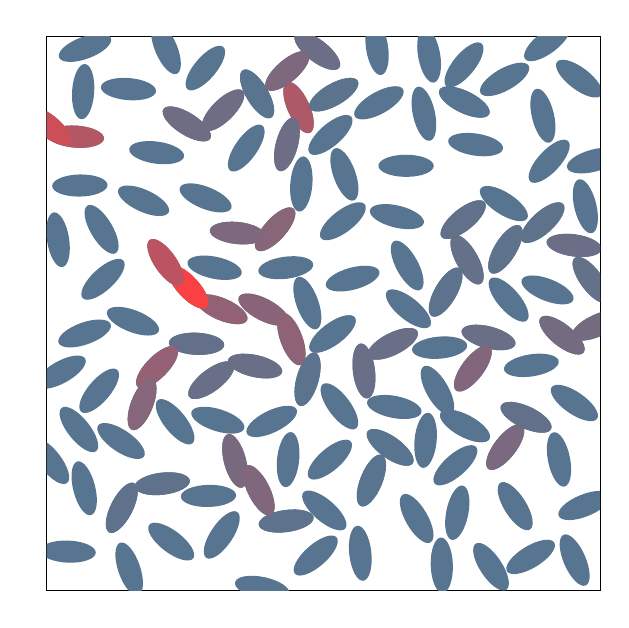
\begin{tikzpicture}

\definecolor{darkgray176}{RGB}{176,176,176}
\definecolor{gray116107129}{RGB}{116,107,129}
\definecolor{gray121105127}{RGB}{121,105,127}
\definecolor{gray122105127}{RGB}{122,105,127}
\definecolor{gray126104125}{RGB}{126,104,125}
\definecolor{gray129103124}{RGB}{129,103,124}
\definecolor{gray131102123}{RGB}{131,102,123}
\definecolor{gray133102122}{RGB}{133,102,122}
\definecolor{gray136101120}{RGB}{136,101,120}
\definecolor{gray137100120}{RGB}{137,100,120}
\definecolor{gray14398117}{RGB}{143,98,117}
\definecolor{gray14698116}{RGB}{146,98,116}
\definecolor{gray14797115}{RGB}{147,97,115}
\definecolor{indianred17389103}{RGB}{173,89,103}
\definecolor{indianred17987100}{RGB}{179,87,100}
\definecolor{indianred1878496}{RGB}{187,84,96}
\definecolor{indianred2047988}{RGB}{204,79,88}
\definecolor{slategray100112137}{RGB}{100,112,137}
\definecolor{slategray101112137}{RGB}{101,112,137}
\definecolor{slategray104111135}{RGB}{104,111,135}
\definecolor{slategray105111135}{RGB}{105,111,135}
\definecolor{slategray106110135}{RGB}{106,110,135}
\definecolor{slategray107110134}{RGB}{107,110,134}
\definecolor{slategray109109133}{RGB}{109,109,133}
\definecolor{slategray110109132}{RGB}{110,109,132}
\definecolor{slategray87117144}{RGB}{87,117,144}
\definecolor{slategray88116143}{RGB}{88,116,143}
\definecolor{slategray90115142}{RGB}{90,115,142}
\definecolor{slategray92115141}{RGB}{92,115,141}
\definecolor{slategray93114141}{RGB}{93,114,141}
\definecolor{slategray94114140}{RGB}{94,114,140}
\definecolor{slategray95114140}{RGB}{95,114,140}
\definecolor{slategray96113139}{RGB}{96,113,139}
\definecolor{slategray98113138}{RGB}{98,113,138}
\definecolor{slategray99112138}{RGB}{99,112,138}
\definecolor{tomato2496568}{RGB}{249,65,68}

\begin{axis}[
    x=2, y=2,
    x grid style={darkgray176},
    xmin=0, xmax=100,
    y grid style={darkgray176},
    ymin=0, ymax=100,
    tick style={draw=none},
    yticklabels={,,},
    xtick
]
\draw[draw=none,fill=slategray87117144,rotate around={40.875524397656:(axis cs:51.1648570437529,23.6259558337609)}] (axis cs:51.1648570437529,23.6259558337609) ellipse (5 and 2);
\draw[draw=none,fill=slategray87117144,rotate around={-66.4590190945365:(axis cs:95.3923133763875,5.47385304205921)}] (axis cs:95.3923133763875,5.47385304205921) ellipse (5 and 2);
\draw[draw=none,fill=slategray87117144,rotate around={169.142589488559:(axis cs:62.8080085056951,33.1351102206122)}] (axis cs:62.8080085056951,33.1351102206122) ellipse (5 and 2);
\draw[draw=none,fill=slategray87117144,rotate around={54.76704895347:(axis cs:36.0582832218256,79.9139520077893)}] (axis cs:36.0582832218256,79.9139520077893) ellipse (5 and 2);
\draw[draw=none,fill=slategray87117144,rotate around={236.000822089611:(axis cs:31.6301764348252,10.0221267751306)}] (axis cs:31.6301764348252,10.0221267751306) ellipse (5 and 2);
\draw[draw=none,fill=slategray87117144,rotate around={300.641690552006:(axis cs:9.91827488846223,65.2253347675313)}] (axis cs:9.91827488846223,65.2253347675313) ellipse (5 and 2);
\draw[draw=none,fill=slategray87117144,rotate around={357.510522881053:(axis cs:27.0778484805433,44.5519123746982)}] (axis cs:27.0778484805433,44.5519123746982) ellipse (5 and 2);
\draw[draw=none,fill=slategray87117144,rotate around={108.910603599823:(axis cs:14.9053897259472,3.88494678234319)}] (axis cs:14.9053897259472,3.88494678234319) ellipse (5 and 2);
\draw[draw=none,fill=slategray87117144,rotate around={-37.7307808746485:(axis cs:48.8864089798238,97.4660543331289)}] (axis cs:48.8864089798238,97.4660543331289) ellipse (5 and 2);
\draw[draw=none,fill=slategray87117144,rotate around={199.544898629417:(axis cs:6.85776851358217,46.4144909609057)}] (axis cs:6.85776851358217,46.4144909609057) ellipse (5 and 2);
\draw[draw=none,fill=slategray87117144,rotate around={38.8860456833893:(axis cs:75.2513413014506,66.9850881519774)}] (axis cs:75.2513413014506,66.9850881519774) ellipse (5 and 2);
\draw[draw=none,fill=slategray87117144,rotate around={154.96380036007:(axis cs:86.6130373102721,31.2634461865813)}] (axis cs:86.6130373102721,31.2634461865813) ellipse (5 and 2);
\draw[draw=none,fill=slategray87117144,rotate around={104.139340572916:(axis cs:6.77953471639772,18.4437313366528)}] (axis cs:6.77953471639772,18.4437313366528) ellipse (5 and 2);
\draw[draw=none,fill=slategray87117144,rotate around={311.000849036147:(axis cs:83.4654190213938,52.537837006355)}] (axis cs:83.4654190213938,52.537837006355) ellipse (5 and 2);
\draw[draw=none,fill=slategray87117144,rotate around={279.892492898966:(axis cs:69.0980894443388,96.6740614205579)}] (axis cs:69.0980894443388,96.6740614205579) ellipse (5 and 2);
\draw[draw=none,fill=slategray87117144,rotate around={-130.216505383211:(axis cs:28.6679961981753,94.364671765754)}] (axis cs:28.6679961981753,94.364671765754) ellipse (5 and 2);
\draw[draw=none,fill=slategray87117144,rotate around={-164.971056227453:(axis cs:55.2753138182248,56.327912138789)}] (axis cs:55.2753138182248,56.327912138789) ellipse (5 and 2);
\draw[draw=none,fill=slategray87117144,rotate around={308.793845484111:(axis cs:23.1989305908088,30.4662840276625)}] (axis cs:23.1989305908088,30.4662840276625) ellipse (5 and 2);
\draw[draw=none,fill=slategray87117144,rotate around={226.963248530117:(axis cs:90.7849493111724,77.5294204413838)}] (axis cs:90.7849493111724,77.5294204413838) ellipse (5 and 2);
\draw[draw=none,fill=slategray87117144,rotate around={-138.927724153564:(axis cs:51.269646493792,82.2836612231218)}] (axis cs:51.269646493792,82.2836612231218) ellipse (5 and 2);
\draw[draw=none,fill=slategray87117144,rotate around={228.03436683592:(axis cs:41.275195491544,65.2411459009429)}] (axis cs:41.275195491544,65.2411459009429) ellipse (5 and 2);
\draw[draw=none,fill=slategray87117144,rotate around={-83.8467282757603:(axis cs:56.6627330715516,6.70722482730468)}] (axis cs:56.6627330715516,6.70722482730468) ellipse (5 and 2);
\draw[draw=none,fill=slategray87117144,rotate around={332.572256044551:(axis cs:39.1797517681094,50.7301691262803)}] (axis cs:39.1797517681094,50.7301691262803) ellipse (5 and 2);
\draw[draw=none,fill=slategray87117144,rotate around={122.318923191082:(axis cs:84.6472542176159,15.2188088241548)}] (axis cs:84.6472542176159,15.2188088241548) ellipse (5 and 2);
\draw[draw=none,fill=slategray87117144,rotate around={-4.54693216158587:(axis cs:14.7764710616188,90.566171512453)}] (axis cs:14.7764710616188,90.566171512453) ellipse (5 and 2);
\draw[draw=none,fill=slategray87117144,rotate around={-21.8725131213154:(axis cs:28.709709701133,70.9127160345857)}] (axis cs:28.709709701133,70.9127160345857) ellipse (5 and 2);
\draw[draw=none,fill=slategray87117144,rotate around={221.478895057041:(axis cs:73.8427411857254,22.6004652177574)}] (axis cs:73.8427411857254,22.6004652177574) ellipse (5 and 2);
\draw[draw=none,fill=slategray87117144,rotate around={-55.102641904684:(axis cs:21.489988879914,59.2319853166713)}] (axis cs:21.489988879914,59.2319853166713) ellipse (5 and 2);
\draw[draw=none,fill=slategray87117144,rotate around={52.9222554698714:(axis cs:76.9983128586217,40.0903088333724)}] (axis cs:76.9983128586217,40.0903088333724) ellipse (5 and 2);
\draw[draw=none,fill=slategray87117144,rotate around={306.391442001627:(axis cs:98.3997218945295,56.0705500691865)}] (axis cs:98.3997218945295,56.0705500691865) ellipse (5 and 2);
\draw[draw=none,fill=slategray87117144,rotate around={-8.60683008931439:(axis cs:77.4953026604655,80.5416255463529)}] (axis cs:77.4953026604655,80.5416255463529) ellipse (5 and 2);
\draw[draw=none,fill=slategray87117144,rotate around={168.17749561288:(axis cs:38.9376701355802,0.428036392048081)}] (axis cs:38.9376701355802,0.428036392048081) ellipse (5 and 2);
\draw[draw=none,fill=slategray87117144,rotate around={229.480941632018:(axis cs:9.4861131262426,36.0644385772206)}] (axis cs:9.4861131262426,36.0644385772206) ellipse (5 and 2);
\draw[draw=none,fill=slategray87117144,rotate around={-7.814923886868:(axis cs:19.8702399861557,79.0872178323864)}] (axis cs:19.8702399861557,79.0872178323864) ellipse (5 and 2);
\draw[draw=none,fill=slategray87117144,rotate around={-37.1835835055139:(axis cs:96.1850969775845,92.4581970217138)}] (axis cs:96.1850969775845,92.4581970217138) ellipse (5 and 2);
\draw[draw=none,fill=slategray87117144,rotate around={209.583415157915:(axis cs:82.7393360270504,92.3201511731193)}] (axis cs:82.7393360270504,92.3201511731193) ellipse (5 and 2);
\draw[draw=none,fill=slategray87117144,rotate around={104.838451932718:(axis cs:34.0210670909596,23.3894828005381)}] (axis cs:34.0210670909596,23.3894828005381) ellipse (5 and 2);
\draw[draw=none,fill=slategray87117144,rotate around={26.7935329067619:(axis cs:62.5295683323414,44.5376087286481)}] (axis cs:62.5295683323414,44.5376087286481) ellipse (5 and 2);
\draw[draw=none,fill=slategray87117144,rotate around={74.0408494007382:(axis cs:47.1331992388735,38.1422453821823)}] (axis cs:47.1331992388735,38.1422453821823) ellipse (5 and 2);
\draw[draw=none,fill=slategray87117144,rotate around={120.041830190493:(axis cs:66.8490562539512,12.9907281801975)}] (axis cs:66.8490562539512,12.9907281801975) ellipse (5 and 2);
\draw[draw=none,fill=slategray87117144,rotate around={179.836201469774:(axis cs:64.931765486061,76.7077317264092)}] (axis cs:64.931765486061,76.7077317264092) ellipse (5 and 2);
\draw[draw=none,fill=slategray87117144,rotate around={205.918869386299:(axis cs:40.6574710023106,30.527038872411)}] (axis cs:40.6574710023106,30.527038872411) ellipse (5 and 2);
\draw[draw=none,fill=slategray87117144,rotate around={356.032979960394:(axis cs:5.3584154333771,81.9705253612302)}] (axis cs:5.3584154333771,81.9705253612302) ellipse (5 and 2);
\draw[draw=none,fill=slategray87117144,rotate around={217.502805274569:(axis cs:53.5150188020371,66.6929245953547)}] (axis cs:53.5150188020371,66.6929245953547) ellipse (5 and 2);
\draw[draw=none,fill=slategray87117144,rotate around={146.012912436536:(axis cs:13.4361627905018,26.9907808418535)}] (axis cs:13.4361627905018,26.9907808418535) ellipse (5 and 2);
\draw[draw=none,fill=slategray87117144,rotate around={141.191822898119:(axis cs:93.099534251567,46.1012461464536)}] (axis cs:93.099534251567,46.1012461464536) ellipse (5 and 2);
\draw[draw=none,fill=slategray87117144,rotate around={347.448298182513:(axis cs:37.655457090786,40.5277858077949)}] (axis cs:37.655457090786,40.5277858077949) ellipse (5 and 2);
\draw[draw=none,fill=slategray87117144,rotate around={42.2467916561144:(axis cs:89.6097033116025,66.4389656286426)}] (axis cs:89.6097033116025,66.4389656286426) ellipse (5 and 2);
\draw[draw=none,fill=slategray87117144,rotate around={36.5690594263747:(axis cs:51.6444496151172,46.3264488774648)}] (axis cs:51.6444496151172,46.3264488774648) ellipse (5 and 2);
\draw[draw=none,fill=slategray87117144,rotate around={118.43383946572:(axis cs:65.1354001214221,58.6946159996219)}] (axis cs:65.1354001214221,58.6946159996219) ellipse (5 and 2);
\draw[draw=none,fill=slategray87117144,rotate around={-157.972096688729:(axis cs:97.1365449629445,15.3353533580117)}] (axis cs:97.1365449629445,15.3353533580117) ellipse (5 and 2);
\draw[draw=none,fill=slategray87117144,rotate around={-81.5436431228741:(axis cs:59.6935944642747,98.0680523027349)}] (axis cs:59.6935944642747,98.0680523027349) ellipse (5 and 2);
\draw[draw=none,fill=slategray87117144,rotate around={303.527600230737:(axis cs:80.2791124538371,4.27254728684565)}] (axis cs:80.2791124538371,4.27254728684565) ellipse (5 and 2);
\draw[draw=none,fill=slategray87117144,rotate around={145.308237565927:(axis cs:95.3369382447089,33.8581179001304)}] (axis cs:95.3369382447089,33.8581179001304) ellipse (5 and 2);
\draw[draw=none,fill=slategray87117144,rotate around={216.958954702617:(axis cs:90.4335742340216,99.0085860959989)}] (axis cs:90.4335742340216,99.0085860959989) ellipse (5 and 2);
\draw[draw=none,fill=slategray87117144,rotate around={-11.8052215827033:(axis cs:30.3458081425066,58.2895466880682)}] (axis cs:30.3458081425066,58.2895466880682) ellipse (5 and 2);
\draw[draw=none,fill=slategray87117144,rotate around={-150.79357841397:(axis cs:60.0289871985712,88.0891516518833)}] (axis cs:60.0289871985712,88.0891516518833) ellipse (5 and 2);
\draw[draw=none,fill=slategray87117144,rotate around={7.82219451909795:(axis cs:43.2664864181439,12.5275308870877)}] (axis cs:43.2664864181439,12.5275308870877) ellipse (5 and 2);
\draw[draw=none,fill=slategray87117144,rotate around={-137.276735300741:(axis cs:10.1736106292829,56.2000262396982)}] (axis cs:10.1736106292829,56.2000262396982) ellipse (5 and 2);
\draw[draw=none,fill=slategray87117144,rotate around={67.8749047560662:(axis cs:58.6683592162668,19.8476286295022)}] (axis cs:58.6683592162668,19.8476286295022) ellipse (5 and 2);
\draw[draw=none,fill=slategray87117144,rotate around={102.54584680536:(axis cs:68.159478162253,86.1165522946094)}] (axis cs:68.159478162253,86.1165522946094) ellipse (5 and 2);
\draw[draw=none,fill=slategray87117144,rotate around={186.700182184229:(axis cs:20.8903319738877,19.2712563743599)}] (axis cs:20.8903319738877,19.2712563743599) ellipse (5 and 2);
\draw[draw=none,fill=slategray87117144,rotate around={322.738771106181:(axis cs:22.4983671550105,8.81220256864047)}] (axis cs:22.4983671550105,8.81220256864047) ellipse (5 and 2);
\draw[draw=none,fill=slategray87117144,rotate around={120.831008217903:(axis cs:38.0154366441204,89.7060134522339)}] (axis cs:38.0154366441204,89.7060134522339) ellipse (5 and 2);
\draw[draw=none,fill=slategray87117144,rotate around={-94.7401632734999:(axis cs:46.0111622660043,73.4223665159154)}] (axis cs:46.0111622660043,73.4223665159154) ellipse (5 and 2);
\draw[draw=none,fill=slategray87117144,rotate around={78.6294744464105:(axis cs:74.1877488740919,14.0322140964467)}] (axis cs:74.1877488740919,14.0322140964467) ellipse (5 and 2);
\draw[draw=none,fill=slategray87117144,rotate around={239.987837174921:(axis cs:72.0845653719768,53.8847441797323)}] (axis cs:72.0845653719768,53.8847441797323) ellipse (5 and 2);
\draw[draw=none,fill=slategray87117144,rotate around={-76.4247301014236:(axis cs:97.3273675796896,69.3992467919002)}] (axis cs:97.3273675796896,69.3992467919002) ellipse (5 and 2);
\draw[draw=none,fill=slategray87117144,rotate around={155.491999173796:(axis cs:17.5042609086314,70.3897572726332)}] (axis cs:17.5042609086314,70.3897572726332) ellipse (5 and 2);
\draw[draw=none,fill=slategray87117144,rotate around={181.080160549271:(axis cs:5.99253296865709,73.1478194648631)}] (axis cs:5.99253296865709,73.1478194648631) ellipse (5 and 2);
\draw[draw=none,fill=slategray87117144,rotate around={177.63836641255:(axis cs:3.87464319366737,7.00330666870228)}] (axis cs:3.87464319366737,7.00330666870228) ellipse (5 and 2);
\draw[draw=none,fill=slategray87117144,rotate around={-53.1133919577382:(axis cs:52.8904363700566,33.2609646860848)}] (axis cs:52.8904363700566,33.2609646860848) ellipse (5 and 2);
\draw[draw=none,fill=slategray87117144,rotate around={20.2985175352883:(axis cs:6.92042097405333,98.0357219983535)}] (axis cs:6.92042097405333,98.0357219983535) ellipse (5 and 2);
\draw[draw=none,fill=slategray87117144,rotate around={8.74941607123059:(axis cs:87.5727904390436,40.6544596459399)}] (axis cs:87.5727904390436,40.6544596459399) ellipse (5 and 2);
\draw[draw=none,fill=slategray87117144,rotate around={-88.2659511424452:(axis cs:71.3863135273704,4.55472065274701)}] (axis cs:71.3863135273704,4.55472065274701) ellipse (5 and 2);
\draw[draw=none,fill=slategray87117144,rotate around={346.48603050339:(axis cs:63.2735338538812,67.5299393853501)}] (axis cs:63.2735338538812,67.5299393853501) ellipse (5 and 2);
\draw[draw=none,fill=slategray87117144,rotate around={158.889253538182:(axis cs:15.5876808521858,48.63568221721)}] (axis cs:15.5876808521858,48.63568221721) ellipse (5 and 2);
\draw[draw=none,fill=slategray87117144,rotate around={327.30075292009:(axis cs:82.6027212049741,69.8860116243992)}] (axis cs:82.6027212049741,69.8860116243992) ellipse (5 and 2);
\draw[draw=none,fill=slategray87117144,rotate around={238.545916429646:(axis cs:82.8871461813991,61.6136972792646)}] (axis cs:82.8871461813991,61.6136972792646) ellipse (5 and 2);
\draw[draw=none,fill=slategray87117144,rotate around={101.350683082049:(axis cs:92.5633337438788,23.6582424684279)}] (axis cs:92.5633337438788,23.6582424684279) ellipse (5 and 2);
\draw[draw=none,fill=slategray87117144,rotate around={-52.2563302269365:(axis cs:0.6305545942345,23.3569521491267)}] (axis cs:0.6305545942345,23.3569521491267) ellipse (5 and 2);
\draw[draw=none,fill=slategray87117144,rotate around={103.526546993261:(axis cs:89.6572451694643,85.7643691259861)}] (axis cs:89.6572451694643,85.7643691259861) ellipse (5 and 2);
\draw[draw=none,fill=slategray87117144,rotate around={209.87459601756:(axis cs:51.8630744035423,89.5601789111925)}] (axis cs:51.8630744035423,89.5601789111925) ellipse (5 and 2);
\draw[draw=none,fill=slategray87117144,rotate around={-67.0061563763847:(axis cs:21.5625640276033,97.9384504282435)}] (axis cs:21.5625640276033,97.9384504282435) ellipse (5 and 2);
\draw[draw=none,fill=slategray87117144,rotate around={225.250027484588:(axis cs:19.9418564689437,40.3345029937303)}] (axis cs:19.9418564689437,40.3345029937303) ellipse (5 and 2);
\draw[draw=none,fill=slategray87117144,rotate around={-25.9111756185369:(axis cs:75.4582473742447,88.2305446873485)}] (axis cs:75.4582473742447,88.2305446873485) ellipse (5 and 2);
\draw[draw=none,fill=slategray87117144,rotate around={4.93971951988574:(axis cs:70.9946199293837,43.8572727329041)}] (axis cs:70.9946199293837,43.8572727329041) ellipse (5 and 2);
\draw[draw=none,fill=slategray87117144,rotate around={342.507960000904:(axis cs:30.9236563739212,30.7504500752328)}] (axis cs:30.9236563739212,30.7504500752328) ellipse (5 and 2);
\draw[draw=none,fill=slategray87117144,rotate around={84.0200656849414:(axis cs:43.6212762118537,23.6270026261015)}] (axis cs:43.6212762118537,23.6270026261015) ellipse (5 and 2);
\draw[draw=none,fill=slategray87117144,rotate around={40.743864401446:(axis cs:43.4816839156329,93.848278455828)}] (axis cs:43.4816839156329,93.848278455828) ellipse (5 and 2);
\draw[draw=none,fill=slategray87117144,rotate around={-40.7503245032577:(axis cs:50.1625567404317,14.4409076105407)}] (axis cs:50.1625567404317,14.4409076105407) ellipse (5 and 2);
\draw[draw=none,fill=slategray87117144,rotate around={41.1802410665004:(axis cs:48.6091299294342,6.29543248460785)}] (axis cs:48.6091299294342,6.29543248460785) ellipse (5 and 2);
\draw[draw=none,fill=slategray87117144,rotate around={-28.0865404577591:(axis cs:75.5820515591917,29.7027050718057)}] (axis cs:75.5820515591917,29.7027050718057) ellipse (5 and 2);
\draw[draw=none,fill=slategray87117144,rotate around={327.739898037879:(axis cs:25.3187967654288,84.2779225769152)}] (axis cs:25.3187967654288,84.2779225769152) ellipse (5 and 2);
\draw[draw=none,fill=slategray87117144,rotate around={15.0131190732381:(axis cs:98.8522080870768,77.6540479835243)}] (axis cs:98.8522080870768,77.6540479835243) ellipse (5 and 2);
\draw[draw=none,fill=slategray87117144,rotate around={50.7721726318709:(axis cs:75.3997114973537,94.9337517573589)}] (axis cs:75.3997114973537,94.9337517573589) ellipse (5 and 2);
\draw[draw=none,fill=slategray87117144,rotate around={62.9698917569343:(axis cs:13.5667546283106,14.9234570935631)}] (axis cs:13.5667546283106,14.9234570935631) ellipse (5 and 2);
\draw[draw=none,fill=slategray87117144,rotate around={128.668742875628:(axis cs:5.82117940832796,29.0640141705424)}] (axis cs:5.82117940832796,29.0640141705424) ellipse (5 and 2);
\draw[draw=none,fill=slategray87117144,rotate around={74.9688562079378:(axis cs:43.4060856328071,80.5860828544838)}] (axis cs:43.4060856328071,80.5860828544838) ellipse (5 and 2);
\draw[draw=none,fill=slategray87117144,rotate around={52.2319018424592:(axis cs:82.8509900740851,25.8877999036146)}] (axis cs:82.8509900740851,25.8877999036146) ellipse (5 and 2);
\draw[draw=none,fill=slategray87117144,rotate around={181.414230087497:(axis cs:29.2322748850495,17.0653890816951)}] (axis cs:29.2322748850495,17.0653890816951) ellipse (5 and 2);
\draw[draw=none,fill=slategray87117144,rotate around={-60.7340808606969:(axis cs:75.9558451584373,59.7401402530375)}] (axis cs:75.9558451584373,59.7401402530375) ellipse (5 and 2);
\draw[draw=none,fill=slategray87117144,rotate around={44.4958755736912:(axis cs:31.8683677012395,86.733876461928)}] (axis cs:31.8683677012395,86.733876461928) ellipse (5 and 2);
\draw[draw=none,fill=slategray87117144,rotate around={217.157361063453:(axis cs:29.7357032583281,37.9831791103198)}] (axis cs:29.7357032583281,37.9831791103198) ellipse (5 and 2);
\draw[draw=none,fill=slategray87117144,rotate around={24.5084900667027:(axis cs:99.5102200385416,47.8756611577218)}] (axis cs:99.5102200385416,47.8756611577218) ellipse (5 and 2);
\draw[draw=none,fill=slategray87117144,rotate around={84.450293826115:(axis cs:68.4619092478204,27.1109468312976)}] (axis cs:68.4619092478204,27.1109468312976) ellipse (5 and 2);
\draw[draw=none,fill=slategray87117144,rotate around={-7.88487995684557:(axis cs:95.2858383734032,62.3266404649775)}] (axis cs:95.2858383734032,62.3266404649775) ellipse (5 and 2);
\draw[draw=none,fill=slategray87117144,rotate around={68.5293203445412:(axis cs:17.2374963638027,33.6555851243459)}] (axis cs:17.2374963638027,33.6555851243459) ellipse (5 and 2);
\draw[draw=none,fill=slategray87117144,rotate around={-38.9329886270601:(axis cs:65.3600719485993,50.8778816075265)}] (axis cs:65.3600719485993,50.8778816075265) ellipse (5 and 2);
\draw[draw=none,fill=slategray87117144,rotate around={109.964585475777:(axis cs:53.7920454584963,75.1628372306203)}] (axis cs:53.7920454584963,75.1628372306203) ellipse (5 and 2);
\draw[draw=none,fill=slategray87117144,rotate around={296.483689399504:(axis cs:38.3259409414495,18.0703640647012)}] (axis cs:38.3259409414495,18.0703640647012) ellipse (5 and 2);
\draw[draw=none,fill=slategray87117144,rotate around={98.9886603713854:(axis cs:2.0609281288955,63.3515859245974)}] (axis cs:2.0609281288955,63.3515859245974) ellipse (5 and 2);
\draw[draw=none,fill=slategray87117144,rotate around={-60.1864137860269:(axis cs:70.6063980373099,36.1294956905252)}] (axis cs:70.6063980373099,36.1294956905252) ellipse (5 and 2);
\draw[draw=none,fill=slategray87117144,rotate around={7.45907132378514:(axis cs:43.2041794633294,58.2919575484574)}] (axis cs:43.2041794633294,58.2919575484574) ellipse (5 and 2);
\draw[draw=none,fill=slategray87117144,rotate around={-150.805570229792:(axis cs:2.59629009912912,39.4273281093086)}] (axis cs:2.59629009912912,39.4273281093086) ellipse (5 and 2);
\draw[draw=none,fill=slategray87117144,rotate around={110.401459638463:(axis cs:44.2190784216896,45.4090333894323)}] (axis cs:44.2190784216896,45.4090333894323) ellipse (5 and 2);
\draw[draw=none,fill=slategray87117144,rotate around={165.479594819256:(axis cs:79.8254930862283,45.695082292786)}] (axis cs:79.8254930862283,45.695082292786) ellipse (5 and 2);
\draw[draw=none,fill=slategray87117144,rotate around={31.1725833199527:(axis cs:87.4373609727411,6.04881734088438)}] (axis cs:87.4373609727411,6.04881734088438) ellipse (5 and 2);
\draw[draw=none,fill=slategray87117144,rotate around={-70.1957354987784:(axis cs:47.0970810984207,51.9098685597701)}] (axis cs:47.0970810984207,51.9098685597701) ellipse (5 and 2);
\draw[draw=none,fill=slategray87117144,rotate around={114.36489015491:(axis cs:45.5072351456916,87.2260394722316)}] (axis cs:45.5072351456916,87.2260394722316) ellipse (5 and 2);
\draw[draw=none,fill=slategray87117144,rotate around={144.642164032275:(axis cs:62.0538143034099,25.8310162619939)}] (axis cs:62.0538143034099,25.8310162619939) ellipse (5 and 2);
\draw[draw=none,fill=slategray87117144,rotate around={-93.6933068134454:(axis cs:6.58928251442549,90.1107021772193)}] (axis cs:6.58928251442549,90.1107021772193) ellipse (5 and 2);
\draw[draw=none,fill=slategray87117144,rotate around={158.441594926307:(axis cs:90.4876843383663,54.2808838624761)}] (axis cs:90.4876843383663,54.2808838624761) ellipse (5 and 2);
\draw[draw=none,fill=slategray87117144,rotate around={97.0677707946229:(axis cs:57.3248447541711,39.6397099148725)}] (axis cs:57.3248447541711,39.6397099148725) ellipse (5 and 2);
\draw[draw=none,fill=slategray87117144,rotate around={156.770685533351:(axis cs:31.6247114292923,50.7928439263777)}] (axis cs:31.6247114292923,50.7928439263777) ellipse (5 and 2);
\draw[draw=none,fill=slategray87117144,rotate around={140.877023181897:(axis cs:0.363161638545817,83.8967940586702)}] (axis cs:0.363161638545817,83.8967940586702) ellipse (5 and 2);
\draw[draw=none,fill=slategray87117144,rotate around={-5.8464105572286:(axis cs:34.4633576597371,64.5598644351866)}] (axis cs:34.4633576597371,64.5598644351866) ellipse (5 and 2);
\draw[draw=none,fill=slategray87117144,rotate around={132.663714880375:(axis cs:25.5409345295187,54.819251008025)}] (axis cs:25.5409345295187,54.819251008025) ellipse (5 and 2);
\draw[draw=none,fill=gray137100120,rotate around={332.572256044551:(axis cs:39.1797517681094,50.7301691262803)}] (axis cs:39.1797517681094,50.7301691262803) ellipse (5 and 2);
\draw[draw=none,fill=slategray104111135,rotate around={347.448298182513:(axis cs:37.655457090786,40.5277858077949)}] (axis cs:37.655457090786,40.5277858077949) ellipse (5 and 2);
\draw[draw=none,fill=gray136101120,rotate around={228.03436683592:(axis cs:41.275195491544,65.2411459009429)}] (axis cs:41.275195491544,65.2411459009429) ellipse (5 and 2);
\draw[draw=none,fill=gray116107129,rotate around={141.191822898119:(axis cs:93.099534251567,46.1012461464536)}] (axis cs:93.099534251567,46.1012461464536) ellipse (5 and 2);
\draw[draw=none,fill=slategray87117144,rotate around={-28.0865404577591:(axis cs:75.5820515591917,29.7027050718057)}] (axis cs:75.5820515591917,29.7027050718057) ellipse (5 and 2);
\draw[draw=none,fill=slategray110109132,rotate around={327.739898037879:(axis cs:25.3187967654288,84.2779225769152)}] (axis cs:25.3187967654288,84.2779225769152) ellipse (5 and 2);
\draw[draw=none,fill=gray14398117,rotate around={110.401459638463:(axis cs:44.2190784216896,45.4090333894323)}] (axis cs:44.2190784216896,45.4090333894323) ellipse (5 and 2);
\draw[draw=none,fill=slategray104111135,rotate around={165.479594819256:(axis cs:79.8254930862283,45.695082292786)}] (axis cs:79.8254930862283,45.695082292786) ellipse (5 and 2);
\draw[draw=none,fill=slategray87117144,rotate around={36.5690594263747:(axis cs:51.6444496151172,46.3264488774648)}] (axis cs:51.6444496151172,46.3264488774648) ellipse (5 and 2);
\draw[draw=none,fill=slategray96113139,rotate around={62.9698917569343:(axis cs:13.5667546283106,14.9234570935631)}] (axis cs:13.5667546283106,14.9234570935631) ellipse (5 and 2);
\draw[draw=none,fill=indianred17389103,rotate around={114.36489015491:(axis cs:45.5072351456916,87.2260394722316)}] (axis cs:45.5072351456916,87.2260394722316) ellipse (5 and 2);
\draw[draw=none,fill=slategray100112137,rotate around={357.510522881053:(axis cs:27.0778484805433,44.5519123746982)}] (axis cs:27.0778484805433,44.5519123746982) ellipse (5 and 2);
\draw[draw=none,fill=slategray107110134,rotate around={-37.7307808746485:(axis cs:48.8864089798238,97.4660543331289)}] (axis cs:48.8864089798238,97.4660543331289) ellipse (5 and 2);
\draw[draw=none,fill=slategray109109133,rotate around={74.9688562079378:(axis cs:43.4060856328071,80.5860828544838)}] (axis cs:43.4060856328071,80.5860828544838) ellipse (5 and 2);
\draw[draw=none,fill=slategray95114140,rotate around={238.545916429646:(axis cs:82.8871461813991,61.6136972792646)}] (axis cs:82.8871461813991,61.6136972792646) ellipse (5 and 2);
\draw[draw=none,fill=slategray88116143,rotate around={144.642164032275:(axis cs:62.0538143034099,25.8310162619939)}] (axis cs:62.0538143034099,25.8310162619939) ellipse (5 and 2);
\draw[draw=none,fill=gray122105127,rotate around={52.2319018424592:(axis cs:82.8509900740851,25.8877999036146)}] (axis cs:82.8509900740851,25.8877999036146) ellipse (5 and 2);
\draw[draw=none,fill=slategray94114140,rotate around={7.82219451909795:(axis cs:43.2664864181439,12.5275308870877)}] (axis cs:43.2664864181439,12.5275308870877) ellipse (5 and 2);
\draw[draw=none,fill=slategray95114140,rotate around={42.2467916561144:(axis cs:89.6097033116025,66.4389656286426)}] (axis cs:89.6097033116025,66.4389656286426) ellipse (5 and 2);
\draw[draw=none,fill=slategray101112137,rotate around={-60.7340808606969:(axis cs:75.9558451584373,59.7401402530375)}] (axis cs:75.9558451584373,59.7401402530375) ellipse (5 and 2);
\draw[draw=none,fill=slategray88116143,rotate around={67.8749047560662:(axis cs:58.6683592162668,19.8476286295022)}] (axis cs:58.6683592162668,19.8476286295022) ellipse (5 and 2);
\draw[draw=none,fill=slategray105111135,rotate around={97.0677707946229:(axis cs:57.3248447541711,39.6397099148725)}] (axis cs:57.3248447541711,39.6397099148725) ellipse (5 and 2);
\draw[draw=none,fill=slategray110109132,rotate around={44.4958755736912:(axis cs:31.8683677012395,86.733876461928)}] (axis cs:31.8683677012395,86.733876461928) ellipse (5 and 2);
\draw[draw=none,fill=slategray92115141,rotate around={209.87459601756:(axis cs:51.8630744035423,89.5601789111925)}] (axis cs:51.8630744035423,89.5601789111925) ellipse (5 and 2);
\draw[draw=none,fill=gray14698116,rotate around={156.770685533351:(axis cs:31.6247114292923,50.7928439263777)}] (axis cs:31.6247114292923,50.7928439263777) ellipse (5 and 2);
\draw[draw=none,fill=slategray104111135,rotate around={217.157361063453:(axis cs:29.7357032583281,37.9831791103198)}] (axis cs:29.7357032583281,37.9831791103198) ellipse (5 and 2);
\draw[draw=none,fill=slategray96113139,rotate around={186.700182184229:(axis cs:20.8903319738877,19.2712563743599)}] (axis cs:20.8903319738877,19.2712563743599) ellipse (5 and 2);
\draw[draw=none,fill=indianred17987100,rotate around={356.032979960394:(axis cs:5.3584154333771,81.9705253612302)}] (axis cs:5.3584154333771,81.9705253612302) ellipse (5 and 2);
\draw[draw=none,fill=indianred2047988,rotate around={140.877023181897:(axis cs:0.363161638545817,83.8967940586702)}] (axis cs:0.363161638545817,83.8967940586702) ellipse (5 and 2);
\draw[draw=none,fill=slategray101112137,rotate around={306.391442001627:(axis cs:98.3997218945295,56.0705500691865)}] (axis cs:98.3997218945295,56.0705500691865) ellipse (5 and 2);
\draw[draw=none,fill=gray116107129,rotate around={24.5084900667027:(axis cs:99.5102200385416,47.8756611577218)}] (axis cs:99.5102200385416,47.8756611577218) ellipse (5 and 2);
\draw[draw=none,fill=gray14797115,rotate around={225.250027484588:(axis cs:19.9418564689437,40.3345029937303)}] (axis cs:19.9418564689437,40.3345029937303) ellipse (5 and 2);
\draw[draw=none,fill=gray126104125,rotate around={-5.8464105572286:(axis cs:34.4633576597371,64.5598644351866)}] (axis cs:34.4633576597371,64.5598644351866) ellipse (5 and 2);
\draw[draw=none,fill=slategray90115142,rotate around={120.831008217903:(axis cs:38.0154366441204,89.7060134522339)}] (axis cs:38.0154366441204,89.7060134522339) ellipse (5 and 2);
\draw[draw=none,fill=gray131102123,rotate around={52.9222554698714:(axis cs:76.9983128586217,40.0903088333724)}] (axis cs:76.9983128586217,40.0903088333724) ellipse (5 and 2);
\draw[draw=none,fill=slategray98113138,rotate around={38.8860456833893:(axis cs:75.2513413014506,66.9850881519774)}] (axis cs:75.2513413014506,66.9850881519774) ellipse (5 and 2);
\draw[draw=none,fill=tomato2496568,rotate around={132.663714880375:(axis cs:25.5409345295187,54.819251008025)}] (axis cs:25.5409345295187,54.819251008025) ellipse (5 and 2);
\draw[draw=none,fill=slategray87117144,rotate around={-25.9111756185369:(axis cs:75.4582473742447,88.2305446873485)}] (axis cs:75.4582473742447,88.2305446873485) ellipse (5 and 2);
\draw[draw=none,fill=slategray107110134,rotate around={-7.88487995684557:(axis cs:95.2858383734032,62.3266404649775)}] (axis cs:95.2858383734032,62.3266404649775) ellipse (5 and 2);
\draw[draw=none,fill=indianred1878496,rotate around={-55.102641904684:(axis cs:21.489988879914,59.2319853166713)}] (axis cs:21.489988879914,59.2319853166713) ellipse (5 and 2);
\draw[draw=none,fill=slategray99112138,rotate around={154.96380036007:(axis cs:86.6130373102721,31.2634461865813)}] (axis cs:86.6130373102721,31.2634461865813) ellipse (5 and 2);
\draw[draw=none,fill=slategray92115141,rotate around={74.0408494007382:(axis cs:47.1331992388735,38.1422453821823)}] (axis cs:47.1331992388735,38.1422453821823) ellipse (5 and 2);
\draw[draw=none,fill=gray133102122,rotate around={68.5293203445412:(axis cs:17.2374963638027,33.6555851243459)}] (axis cs:17.2374963638027,33.6555851243459) ellipse (5 and 2);
\draw[draw=none,fill=slategray93114141,rotate around={239.987837174921:(axis cs:72.0845653719768,53.8847441797323)}] (axis cs:72.0845653719768,53.8847441797323) ellipse (5 and 2);
\draw[draw=none,fill=slategray106110135,rotate around={26.7935329067619:(axis cs:62.5295683323414,44.5376087286481)}] (axis cs:62.5295683323414,44.5376087286481) ellipse (5 and 2);
\draw[draw=none,fill=gray121105127,rotate around={104.838451932718:(axis cs:34.0210670909596,23.3894828005381)}] (axis cs:34.0210670909596,23.3894828005381) ellipse (5 and 2);
\draw[draw=none,fill=gray126104125,rotate around={40.743864401446:(axis cs:43.4816839156329,93.848278455828)}] (axis cs:43.4816839156329,93.848278455828) ellipse (5 and 2);
\draw[draw=none,fill=gray129103124,rotate around={296.483689399504:(axis cs:38.3259409414495,18.0703640647012)}] (axis cs:38.3259409414495,18.0703640647012) ellipse (5 and 2);
\end{axis}

\end{tikzpicture}
}
    \caption{Barva prekritih elips je odvisna od njihove energije.}
    \label{fig:energija}
\end{figure}
\subsection{Različni koraki rasti}
Pri isti začetni porazdelitvi točk, večkrat zgeneriramo porazdelitve elips z~različnimi
začetnimi naključnimi orientacijami. Na sliki~\ref{fig:delta_a_01} je prikazan tak primer
pri koraku rasti $\Delta a = 0,1$ pri začetni velikosti $a_0 = 5$ in končni $a = 8$. 
Razmerje med polosmi je $a/b = 5/2$.
\begin{figure}[!ht]
    \centering
    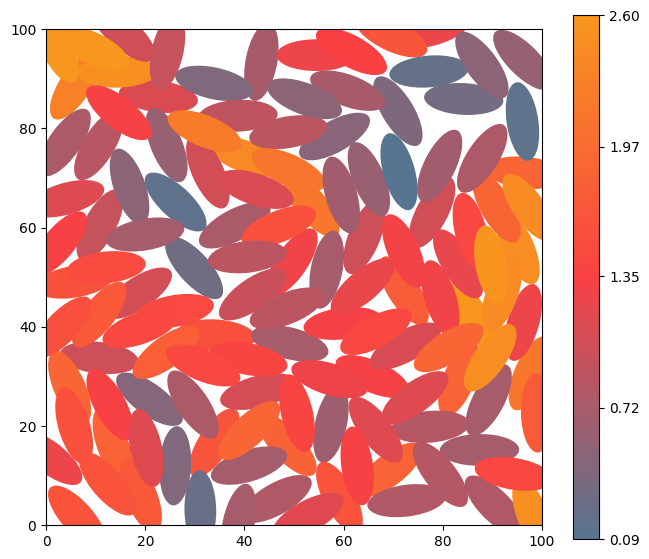
\includegraphics[width=0.38\textwidth]{./figures/runs/delta_a_01/run01}
    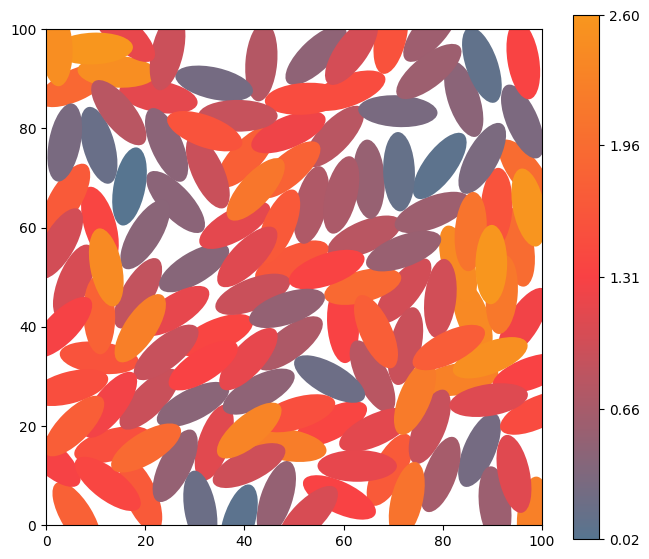
\includegraphics[width=0.38\textwidth]{./figures/runs/delta_a_01/run02}
    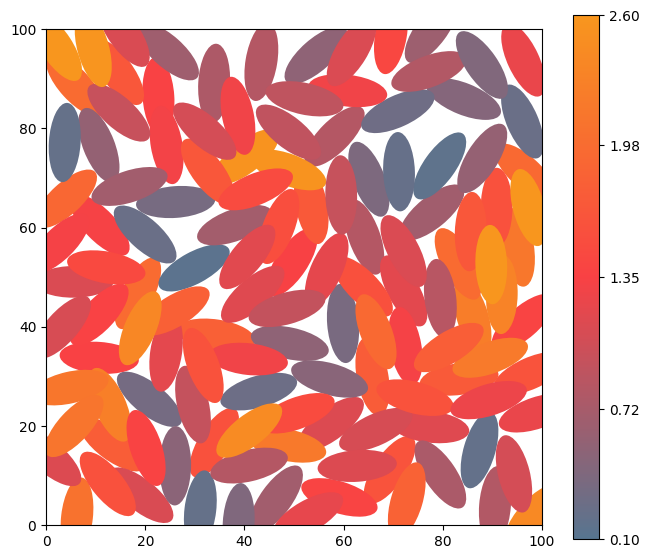
\includegraphics[width=0.38\textwidth]{./figures/runs/delta_a_01/run03}
    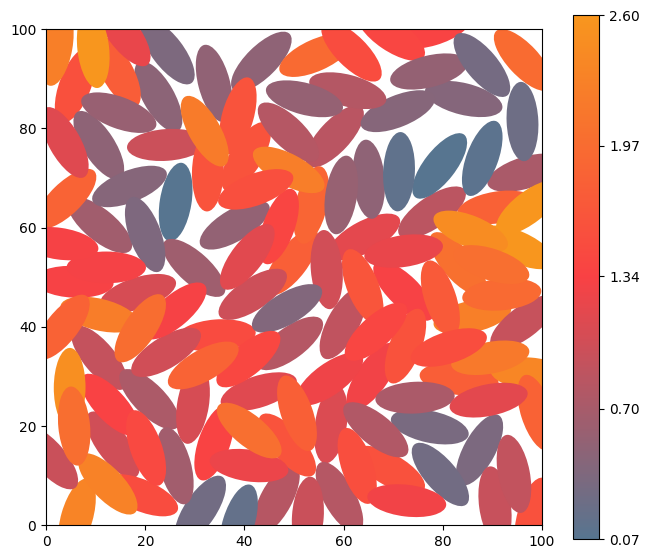
\includegraphics[width=0.38\textwidth]{./figures/runs/delta_a_01/run04}
    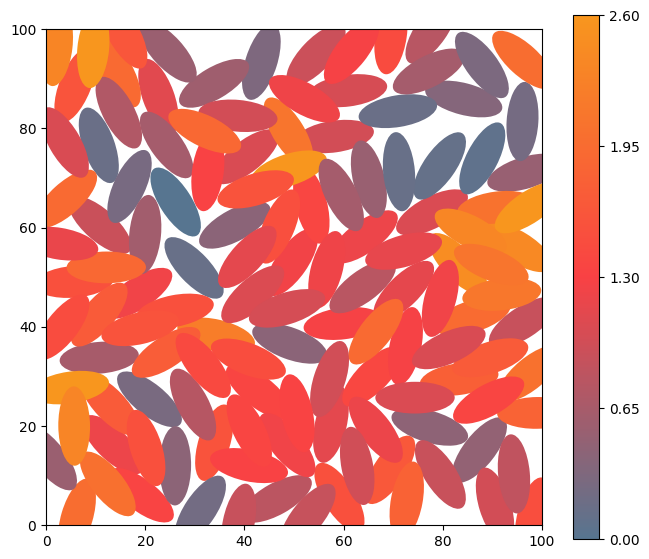
\includegraphics[width=0.38\textwidth]{./figures/runs/delta_a_01/run05}
    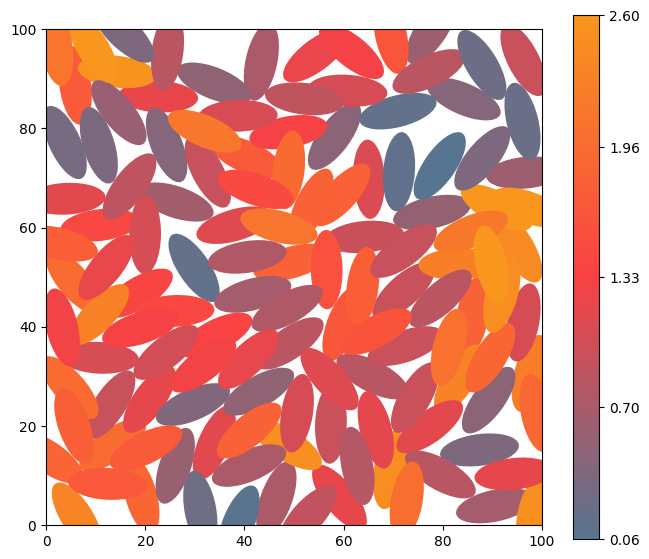
\includegraphics[width=0.38\textwidth]{./figures/runs/delta_a_01/run06}
    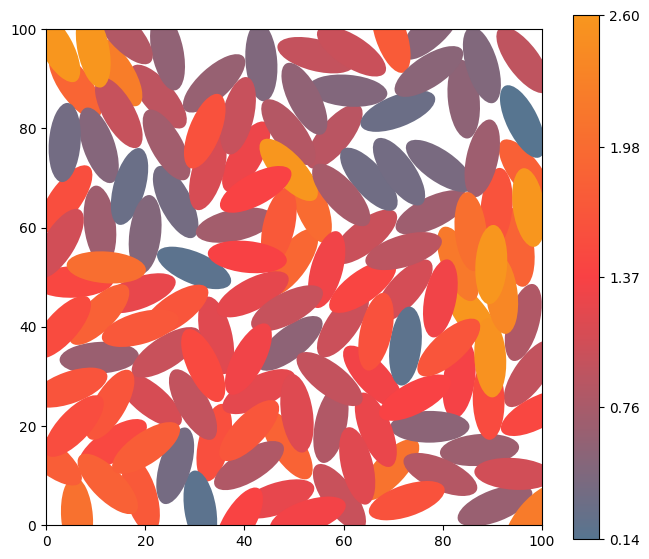
\includegraphics[width=0.38\textwidth]{./figures/runs/delta_a_01/run07}
    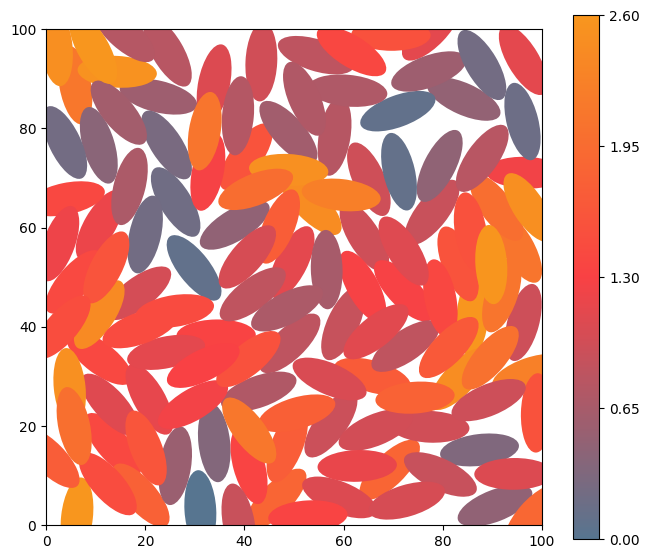
\includegraphics[width=0.38\textwidth]{./figures/runs/delta_a_01/run08}
    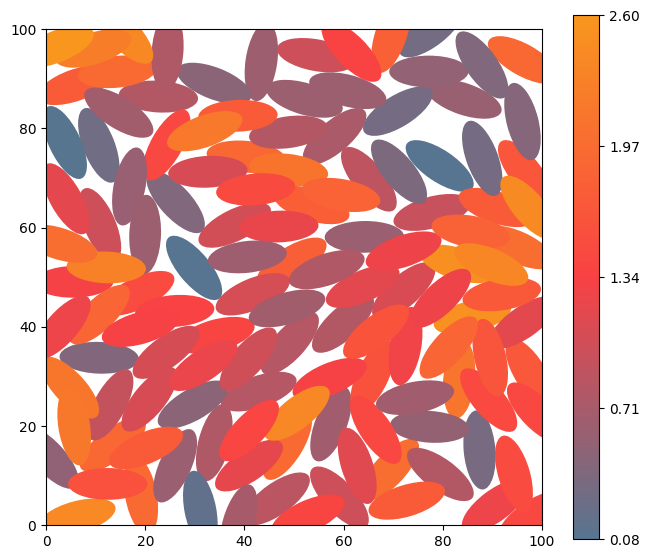
\includegraphics[width=0.38\textwidth]{./figures/runs/delta_a_01/run09}
    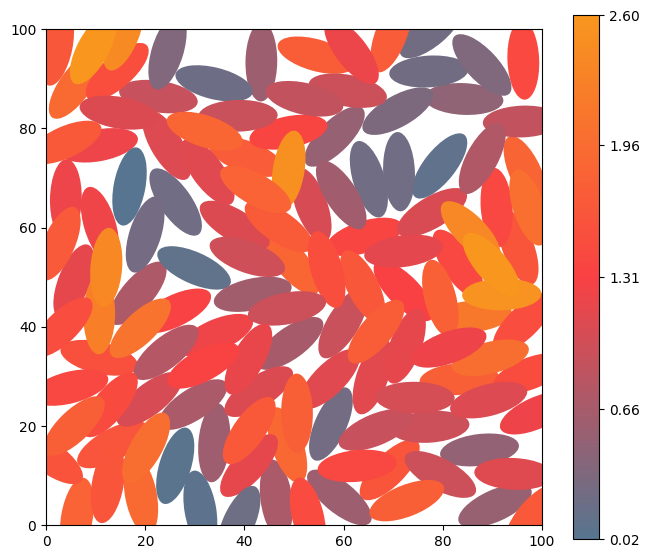
\includegraphics[width=0.38\textwidth]{./figures/runs/delta_a_01/run10}
    \caption{Razvoj sistema iz iste začetne porazdelitve $128$ elips in desetih različnih
    začetnih naključnih orientacijah. Velikost koraka je $\Delta a = 0,1$.}
    \label{fig:delta_a_01}
\end{figure}
Spodaj so prikazani grafi energije, povprečnega števila kontaktov na elipso, orientacijske
korelacijske funkcije in števila sprejetih in zavrnjenih rotacij med računanjem 
(če je med poskusom relaksacije sistema vrednost energije padla na $0$, se je računanje 
prekinilo -- zato se je kdaj zgodilo, da vsota sprejtih in zavrnjenih rotacij ni konstantna).
\begin{figure}
    \centering
    \resizebox{.45\textwidth}{!}{% GNUPLOT: LaTeX picture with Postscript
\begingroup
  \makeatletter
  \providecommand\color[2][]{%
    \GenericError{(gnuplot) \space\space\space\@spaces}{%
      Package color not loaded in conjunction with
      terminal option `colourtext'%
    }{See the gnuplot documentation for explanation.%
    }{Either use 'blacktext' in gnuplot or load the package
      color.sty in LaTeX.}%
    \renewcommand\color[2][]{}%
  }%
  \providecommand\includegraphics[2][]{%
    \GenericError{(gnuplot) \space\space\space\@spaces}{%
      Package graphicx or graphics not loaded%
    }{See the gnuplot documentation for explanation.%
    }{The gnuplot epslatex terminal needs graphicx.sty or graphics.sty.}%
    \renewcommand\includegraphics[2][]{}%
  }%
  \providecommand\rotatebox[2]{#2}%
  \@ifundefined{ifGPcolor}{%
    \newif\ifGPcolor
    \GPcolortrue
  }{}%
  \@ifundefined{ifGPblacktext}{%
    \newif\ifGPblacktext
    \GPblacktexttrue
  }{}%
  % define a \g@addto@macro without @ in the name:
  \let\gplgaddtomacro\g@addto@macro
  % define empty templates for all commands taking text:
  \gdef\gplbacktext{}%
  \gdef\gplfronttext{}%
  \makeatother
  \ifGPblacktext
    % no textcolor at all
    \def\colorrgb#1{}%
    \def\colorgray#1{}%
  \else
    % gray or color?
    \ifGPcolor
      \def\colorrgb#1{\color[rgb]{#1}}%
      \def\colorgray#1{\color[gray]{#1}}%
      \expandafter\def\csname LTw\endcsname{\color{white}}%
      \expandafter\def\csname LTb\endcsname{\color{black}}%
      \expandafter\def\csname LTa\endcsname{\color{black}}%
      \expandafter\def\csname LT0\endcsname{\color[rgb]{1,0,0}}%
      \expandafter\def\csname LT1\endcsname{\color[rgb]{0,1,0}}%
      \expandafter\def\csname LT2\endcsname{\color[rgb]{0,0,1}}%
      \expandafter\def\csname LT3\endcsname{\color[rgb]{1,0,1}}%
      \expandafter\def\csname LT4\endcsname{\color[rgb]{0,1,1}}%
      \expandafter\def\csname LT5\endcsname{\color[rgb]{1,1,0}}%
      \expandafter\def\csname LT6\endcsname{\color[rgb]{0,0,0}}%
      \expandafter\def\csname LT7\endcsname{\color[rgb]{1,0.3,0}}%
      \expandafter\def\csname LT8\endcsname{\color[rgb]{0.5,0.5,0.5}}%
    \else
      % gray
      \def\colorrgb#1{\color{black}}%
      \def\colorgray#1{\color[gray]{#1}}%
      \expandafter\def\csname LTw\endcsname{\color{white}}%
      \expandafter\def\csname LTb\endcsname{\color{black}}%
      \expandafter\def\csname LTa\endcsname{\color{black}}%
      \expandafter\def\csname LT0\endcsname{\color{black}}%
      \expandafter\def\csname LT1\endcsname{\color{black}}%
      \expandafter\def\csname LT2\endcsname{\color{black}}%
      \expandafter\def\csname LT3\endcsname{\color{black}}%
      \expandafter\def\csname LT4\endcsname{\color{black}}%
      \expandafter\def\csname LT5\endcsname{\color{black}}%
      \expandafter\def\csname LT6\endcsname{\color{black}}%
      \expandafter\def\csname LT7\endcsname{\color{black}}%
      \expandafter\def\csname LT8\endcsname{\color{black}}%
    \fi
  \fi
    \setlength{\unitlength}{0.0500bp}%
    \ifx\gptboxheight\undefined%
      \newlength{\gptboxheight}%
      \newlength{\gptboxwidth}%
      \newsavebox{\gptboxtext}%
    \fi%
    \setlength{\fboxrule}{0.5pt}%
    \setlength{\fboxsep}{1pt}%
    \definecolor{tbcol}{rgb}{1,1,1}%
\begin{picture}(7080.00,5660.00)%
    \gplgaddtomacro\gplbacktext{%
      \csname LTb\endcsname%%
      \put(692,767){\makebox(0,0)[r]{\strut{}$0$}}%
      \csname LTb\endcsname%%
      \put(692,1925){\makebox(0,0)[r]{\strut{}$25$}}%
      \csname LTb\endcsname%%
      \put(692,3083){\makebox(0,0)[r]{\strut{}$50$}}%
      \csname LTb\endcsname%%
      \put(692,4241){\makebox(0,0)[r]{\strut{}$75$}}%
      \csname LTb\endcsname%%
      \put(692,5400){\makebox(0,0)[r]{\strut{}$100$}}%
      \csname LTb\endcsname%%
      \put(793,527){\makebox(0,0){\strut{}$5$}}%
      \csname LTb\endcsname%%
      \put(1787,527){\makebox(0,0){\strut{}$5.5$}}%
      \csname LTb\endcsname%%
      \put(2781,527){\makebox(0,0){\strut{}$6$}}%
      \csname LTb\endcsname%%
      \put(3775,527){\makebox(0,0){\strut{}$6.5$}}%
      \csname LTb\endcsname%%
      \put(4769,527){\makebox(0,0){\strut{}$7$}}%
      \csname LTb\endcsname%%
      \put(5763,527){\makebox(0,0){\strut{}$7.5$}}%
      \csname LTb\endcsname%%
      \put(6757,527){\makebox(0,0){\strut{}$8$}}%
    }%
    \gplgaddtomacro\gplfronttext{%
      \csname LTb\endcsname%%
      \put(195,3083){\rotatebox{-270}{\makebox(0,0){\strut{}$u$}}}%
      \csname LTb\endcsname%%
      \put(3775,167){\makebox(0,0){\strut{}$a$}}%
    }%
    \gplbacktext
    \put(0,0){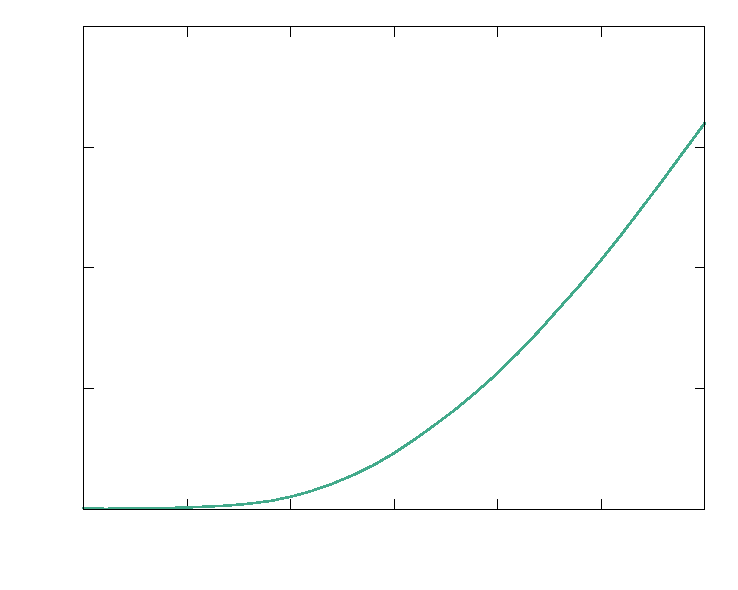
\includegraphics[width={354.00bp},height={283.00bp}]{./gnuplot/growth_a_01_energy_1}}%
    \gplfronttext
  \end{picture}%
\endgroup
}
    \resizebox{.45\textwidth}{!}{% GNUPLOT: LaTeX picture with Postscript
\begingroup
  \makeatletter
  \providecommand\color[2][]{%
    \GenericError{(gnuplot) \space\space\space\@spaces}{%
      Package color not loaded in conjunction with
      terminal option `colourtext'%
    }{See the gnuplot documentation for explanation.%
    }{Either use 'blacktext' in gnuplot or load the package
      color.sty in LaTeX.}%
    \renewcommand\color[2][]{}%
  }%
  \providecommand\includegraphics[2][]{%
    \GenericError{(gnuplot) \space\space\space\@spaces}{%
      Package graphicx or graphics not loaded%
    }{See the gnuplot documentation for explanation.%
    }{The gnuplot epslatex terminal needs graphicx.sty or graphics.sty.}%
    \renewcommand\includegraphics[2][]{}%
  }%
  \providecommand\rotatebox[2]{#2}%
  \@ifundefined{ifGPcolor}{%
    \newif\ifGPcolor
    \GPcolortrue
  }{}%
  \@ifundefined{ifGPblacktext}{%
    \newif\ifGPblacktext
    \GPblacktexttrue
  }{}%
  % define a \g@addto@macro without @ in the name:
  \let\gplgaddtomacro\g@addto@macro
  % define empty templates for all commands taking text:
  \gdef\gplbacktext{}%
  \gdef\gplfronttext{}%
  \makeatother
  \ifGPblacktext
    % no textcolor at all
    \def\colorrgb#1{}%
    \def\colorgray#1{}%
  \else
    % gray or color?
    \ifGPcolor
      \def\colorrgb#1{\color[rgb]{#1}}%
      \def\colorgray#1{\color[gray]{#1}}%
      \expandafter\def\csname LTw\endcsname{\color{white}}%
      \expandafter\def\csname LTb\endcsname{\color{black}}%
      \expandafter\def\csname LTa\endcsname{\color{black}}%
      \expandafter\def\csname LT0\endcsname{\color[rgb]{1,0,0}}%
      \expandafter\def\csname LT1\endcsname{\color[rgb]{0,1,0}}%
      \expandafter\def\csname LT2\endcsname{\color[rgb]{0,0,1}}%
      \expandafter\def\csname LT3\endcsname{\color[rgb]{1,0,1}}%
      \expandafter\def\csname LT4\endcsname{\color[rgb]{0,1,1}}%
      \expandafter\def\csname LT5\endcsname{\color[rgb]{1,1,0}}%
      \expandafter\def\csname LT6\endcsname{\color[rgb]{0,0,0}}%
      \expandafter\def\csname LT7\endcsname{\color[rgb]{1,0.3,0}}%
      \expandafter\def\csname LT8\endcsname{\color[rgb]{0.5,0.5,0.5}}%
    \else
      % gray
      \def\colorrgb#1{\color{black}}%
      \def\colorgray#1{\color[gray]{#1}}%
      \expandafter\def\csname LTw\endcsname{\color{white}}%
      \expandafter\def\csname LTb\endcsname{\color{black}}%
      \expandafter\def\csname LTa\endcsname{\color{black}}%
      \expandafter\def\csname LT0\endcsname{\color{black}}%
      \expandafter\def\csname LT1\endcsname{\color{black}}%
      \expandafter\def\csname LT2\endcsname{\color{black}}%
      \expandafter\def\csname LT3\endcsname{\color{black}}%
      \expandafter\def\csname LT4\endcsname{\color{black}}%
      \expandafter\def\csname LT5\endcsname{\color{black}}%
      \expandafter\def\csname LT6\endcsname{\color{black}}%
      \expandafter\def\csname LT7\endcsname{\color{black}}%
      \expandafter\def\csname LT8\endcsname{\color{black}}%
    \fi
  \fi
    \setlength{\unitlength}{0.0500bp}%
    \ifx\gptboxheight\undefined%
      \newlength{\gptboxheight}%
      \newlength{\gptboxwidth}%
      \newsavebox{\gptboxtext}%
    \fi%
    \setlength{\fboxrule}{0.5pt}%
    \setlength{\fboxsep}{1pt}%
    \definecolor{tbcol}{rgb}{1,1,1}%
\begin{picture}(7080.00,5660.00)%
    \gplgaddtomacro\gplbacktext{%
      \csname LTb\endcsname%%
      \put(692,767){\makebox(0,0)[r]{\strut{}$0$}}%
      \csname LTb\endcsname%%
      \put(692,1925){\makebox(0,0)[r]{\strut{}$0.4$}}%
      \csname LTb\endcsname%%
      \put(692,3083){\makebox(0,0)[r]{\strut{}$0.8$}}%
      \csname LTb\endcsname%%
      \put(692,4241){\makebox(0,0)[r]{\strut{}$1.2$}}%
      \csname LTb\endcsname%%
      \put(692,5400){\makebox(0,0)[r]{\strut{}$1.6$}}%
      \csname LTb\endcsname%%
      \put(793,527){\makebox(0,0){\strut{}$5$}}%
      \csname LTb\endcsname%%
      \put(1787,527){\makebox(0,0){\strut{}$5.5$}}%
      \csname LTb\endcsname%%
      \put(2781,527){\makebox(0,0){\strut{}$6$}}%
      \csname LTb\endcsname%%
      \put(3775,527){\makebox(0,0){\strut{}$6.5$}}%
      \csname LTb\endcsname%%
      \put(4769,527){\makebox(0,0){\strut{}$7$}}%
      \csname LTb\endcsname%%
      \put(5763,527){\makebox(0,0){\strut{}$7.5$}}%
      \csname LTb\endcsname%%
      \put(6757,527){\makebox(0,0){\strut{}$8$}}%
    }%
    \gplgaddtomacro\gplfronttext{%
      \csname LTb\endcsname%%
      \put(195,3083){\rotatebox{-270}{\makebox(0,0){\strut{}$\sigma_{u} / u$}}}%
      \csname LTb\endcsname%%
      \put(3775,167){\makebox(0,0){\strut{}$a$}}%
    }%
    \gplbacktext
    \put(0,0){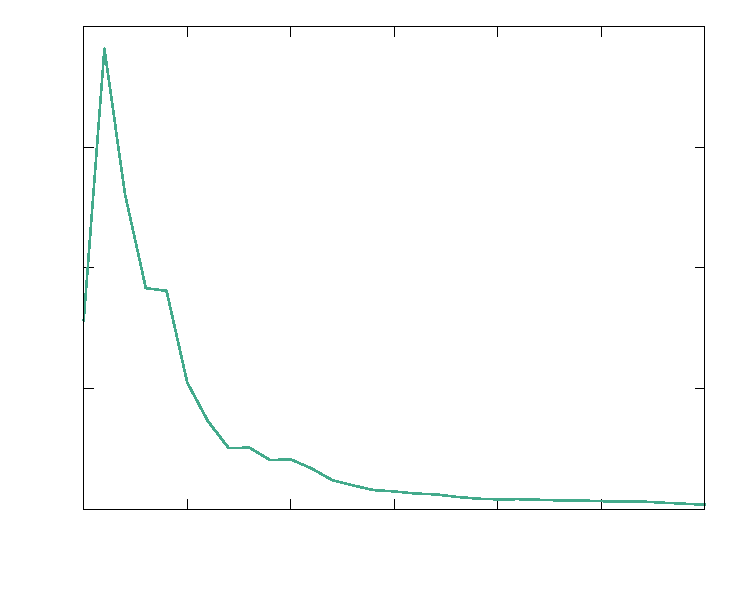
\includegraphics[width={354.00bp},height={283.00bp}]{./gnuplot/growth_a_01_energy_2}}%
    \gplfronttext
  \end{picture}%
\endgroup
}
    \resizebox{.45\textwidth}{!}{% GNUPLOT: LaTeX picture with Postscript
\begingroup
  \makeatletter
  \providecommand\color[2][]{%
    \GenericError{(gnuplot) \space\space\space\@spaces}{%
      Package color not loaded in conjunction with
      terminal option `colourtext'%
    }{See the gnuplot documentation for explanation.%
    }{Either use 'blacktext' in gnuplot or load the package
      color.sty in LaTeX.}%
    \renewcommand\color[2][]{}%
  }%
  \providecommand\includegraphics[2][]{%
    \GenericError{(gnuplot) \space\space\space\@spaces}{%
      Package graphicx or graphics not loaded%
    }{See the gnuplot documentation for explanation.%
    }{The gnuplot epslatex terminal needs graphicx.sty or graphics.sty.}%
    \renewcommand\includegraphics[2][]{}%
  }%
  \providecommand\rotatebox[2]{#2}%
  \@ifundefined{ifGPcolor}{%
    \newif\ifGPcolor
    \GPcolortrue
  }{}%
  \@ifundefined{ifGPblacktext}{%
    \newif\ifGPblacktext
    \GPblacktexttrue
  }{}%
  % define a \g@addto@macro without @ in the name:
  \let\gplgaddtomacro\g@addto@macro
  % define empty templates for all commands taking text:
  \gdef\gplbacktext{}%
  \gdef\gplfronttext{}%
  \makeatother
  \ifGPblacktext
    % no textcolor at all
    \def\colorrgb#1{}%
    \def\colorgray#1{}%
  \else
    % gray or color?
    \ifGPcolor
      \def\colorrgb#1{\color[rgb]{#1}}%
      \def\colorgray#1{\color[gray]{#1}}%
      \expandafter\def\csname LTw\endcsname{\color{white}}%
      \expandafter\def\csname LTb\endcsname{\color{black}}%
      \expandafter\def\csname LTa\endcsname{\color{black}}%
      \expandafter\def\csname LT0\endcsname{\color[rgb]{1,0,0}}%
      \expandafter\def\csname LT1\endcsname{\color[rgb]{0,1,0}}%
      \expandafter\def\csname LT2\endcsname{\color[rgb]{0,0,1}}%
      \expandafter\def\csname LT3\endcsname{\color[rgb]{1,0,1}}%
      \expandafter\def\csname LT4\endcsname{\color[rgb]{0,1,1}}%
      \expandafter\def\csname LT5\endcsname{\color[rgb]{1,1,0}}%
      \expandafter\def\csname LT6\endcsname{\color[rgb]{0,0,0}}%
      \expandafter\def\csname LT7\endcsname{\color[rgb]{1,0.3,0}}%
      \expandafter\def\csname LT8\endcsname{\color[rgb]{0.5,0.5,0.5}}%
    \else
      % gray
      \def\colorrgb#1{\color{black}}%
      \def\colorgray#1{\color[gray]{#1}}%
      \expandafter\def\csname LTw\endcsname{\color{white}}%
      \expandafter\def\csname LTb\endcsname{\color{black}}%
      \expandafter\def\csname LTa\endcsname{\color{black}}%
      \expandafter\def\csname LT0\endcsname{\color{black}}%
      \expandafter\def\csname LT1\endcsname{\color{black}}%
      \expandafter\def\csname LT2\endcsname{\color{black}}%
      \expandafter\def\csname LT3\endcsname{\color{black}}%
      \expandafter\def\csname LT4\endcsname{\color{black}}%
      \expandafter\def\csname LT5\endcsname{\color{black}}%
      \expandafter\def\csname LT6\endcsname{\color{black}}%
      \expandafter\def\csname LT7\endcsname{\color{black}}%
      \expandafter\def\csname LT8\endcsname{\color{black}}%
    \fi
  \fi
    \setlength{\unitlength}{0.0500bp}%
    \ifx\gptboxheight\undefined%
      \newlength{\gptboxheight}%
      \newlength{\gptboxwidth}%
      \newsavebox{\gptboxtext}%
    \fi%
    \setlength{\fboxrule}{0.5pt}%
    \setlength{\fboxsep}{1pt}%
    \definecolor{tbcol}{rgb}{1,1,1}%
\begin{picture}(7080.00,5660.00)%
    \gplgaddtomacro\gplbacktext{%
      \csname LTb\endcsname%%
      \put(491,767){\makebox(0,0)[r]{\strut{}$0$}}%
      \csname LTb\endcsname%%
      \put(491,1796){\makebox(0,0)[r]{\strut{}$1$}}%
      \csname LTb\endcsname%%
      \put(491,2826){\makebox(0,0)[r]{\strut{}$2$}}%
      \csname LTb\endcsname%%
      \put(491,3855){\makebox(0,0)[r]{\strut{}$3$}}%
      \csname LTb\endcsname%%
      \put(491,4885){\makebox(0,0)[r]{\strut{}$4$}}%
      \csname LTb\endcsname%%
      \put(592,527){\makebox(0,0){\strut{}$5$}}%
      \csname LTb\endcsname%%
      \put(1619,527){\makebox(0,0){\strut{}$5.5$}}%
      \csname LTb\endcsname%%
      \put(2647,527){\makebox(0,0){\strut{}$6$}}%
      \csname LTb\endcsname%%
      \put(3675,527){\makebox(0,0){\strut{}$6.5$}}%
      \csname LTb\endcsname%%
      \put(4702,527){\makebox(0,0){\strut{}$7$}}%
      \csname LTb\endcsname%%
      \put(5730,527){\makebox(0,0){\strut{}$7.5$}}%
      \csname LTb\endcsname%%
      \put(6757,527){\makebox(0,0){\strut{}$8$}}%
    }%
    \gplgaddtomacro\gplfronttext{%
      \csname LTb\endcsname%%
      \put(195,3083){\rotatebox{-270}{\makebox(0,0){\strut{}$Z$}}}%
      \csname LTb\endcsname%%
      \put(3674,167){\makebox(0,0){\strut{}$a$}}%
    }%
    \gplbacktext
    \put(0,0){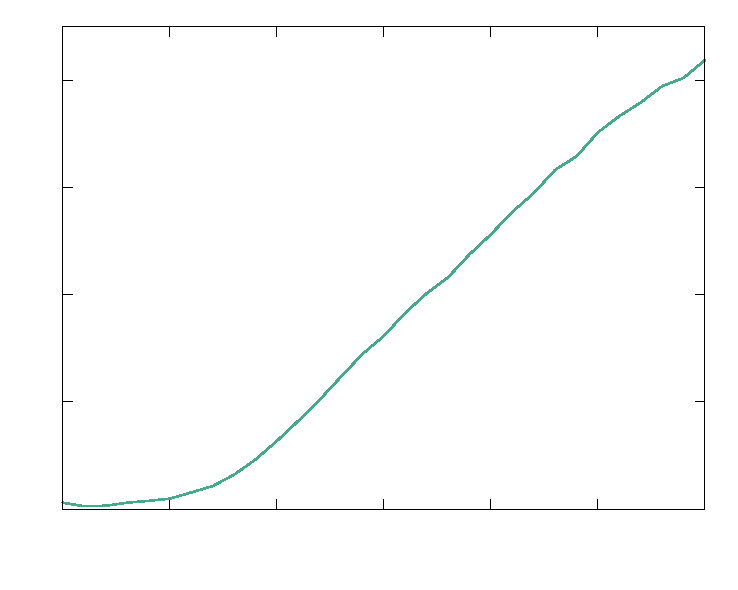
\includegraphics[width={354.00bp},height={283.00bp}]{./gnuplot/growth_a_01_coord_1}}%
    \gplfronttext
  \end{picture}%
\endgroup
}
    \resizebox{.45\textwidth}{!}{% GNUPLOT: LaTeX picture with Postscript
\begingroup
  \makeatletter
  \providecommand\color[2][]{%
    \GenericError{(gnuplot) \space\space\space\@spaces}{%
      Package color not loaded in conjunction with
      terminal option `colourtext'%
    }{See the gnuplot documentation for explanation.%
    }{Either use 'blacktext' in gnuplot or load the package
      color.sty in LaTeX.}%
    \renewcommand\color[2][]{}%
  }%
  \providecommand\includegraphics[2][]{%
    \GenericError{(gnuplot) \space\space\space\@spaces}{%
      Package graphicx or graphics not loaded%
    }{See the gnuplot documentation for explanation.%
    }{The gnuplot epslatex terminal needs graphicx.sty or graphics.sty.}%
    \renewcommand\includegraphics[2][]{}%
  }%
  \providecommand\rotatebox[2]{#2}%
  \@ifundefined{ifGPcolor}{%
    \newif\ifGPcolor
    \GPcolortrue
  }{}%
  \@ifundefined{ifGPblacktext}{%
    \newif\ifGPblacktext
    \GPblacktexttrue
  }{}%
  % define a \g@addto@macro without @ in the name:
  \let\gplgaddtomacro\g@addto@macro
  % define empty templates for all commands taking text:
  \gdef\gplbacktext{}%
  \gdef\gplfronttext{}%
  \makeatother
  \ifGPblacktext
    % no textcolor at all
    \def\colorrgb#1{}%
    \def\colorgray#1{}%
  \else
    % gray or color?
    \ifGPcolor
      \def\colorrgb#1{\color[rgb]{#1}}%
      \def\colorgray#1{\color[gray]{#1}}%
      \expandafter\def\csname LTw\endcsname{\color{white}}%
      \expandafter\def\csname LTb\endcsname{\color{black}}%
      \expandafter\def\csname LTa\endcsname{\color{black}}%
      \expandafter\def\csname LT0\endcsname{\color[rgb]{1,0,0}}%
      \expandafter\def\csname LT1\endcsname{\color[rgb]{0,1,0}}%
      \expandafter\def\csname LT2\endcsname{\color[rgb]{0,0,1}}%
      \expandafter\def\csname LT3\endcsname{\color[rgb]{1,0,1}}%
      \expandafter\def\csname LT4\endcsname{\color[rgb]{0,1,1}}%
      \expandafter\def\csname LT5\endcsname{\color[rgb]{1,1,0}}%
      \expandafter\def\csname LT6\endcsname{\color[rgb]{0,0,0}}%
      \expandafter\def\csname LT7\endcsname{\color[rgb]{1,0.3,0}}%
      \expandafter\def\csname LT8\endcsname{\color[rgb]{0.5,0.5,0.5}}%
    \else
      % gray
      \def\colorrgb#1{\color{black}}%
      \def\colorgray#1{\color[gray]{#1}}%
      \expandafter\def\csname LTw\endcsname{\color{white}}%
      \expandafter\def\csname LTb\endcsname{\color{black}}%
      \expandafter\def\csname LTa\endcsname{\color{black}}%
      \expandafter\def\csname LT0\endcsname{\color{black}}%
      \expandafter\def\csname LT1\endcsname{\color{black}}%
      \expandafter\def\csname LT2\endcsname{\color{black}}%
      \expandafter\def\csname LT3\endcsname{\color{black}}%
      \expandafter\def\csname LT4\endcsname{\color{black}}%
      \expandafter\def\csname LT5\endcsname{\color{black}}%
      \expandafter\def\csname LT6\endcsname{\color{black}}%
      \expandafter\def\csname LT7\endcsname{\color{black}}%
      \expandafter\def\csname LT8\endcsname{\color{black}}%
    \fi
  \fi
    \setlength{\unitlength}{0.0500bp}%
    \ifx\gptboxheight\undefined%
      \newlength{\gptboxheight}%
      \newlength{\gptboxwidth}%
      \newsavebox{\gptboxtext}%
    \fi%
    \setlength{\fboxrule}{0.5pt}%
    \setlength{\fboxsep}{1pt}%
    \definecolor{tbcol}{rgb}{1,1,1}%
\begin{picture}(7080.00,5660.00)%
    \gplgaddtomacro\gplbacktext{%
      \csname LTb\endcsname%%
      \put(692,767){\makebox(0,0)[r]{\strut{}$0$}}%
      \csname LTb\endcsname%%
      \put(692,2192){\makebox(0,0)[r]{\strut{}$0.4$}}%
      \csname LTb\endcsname%%
      \put(692,3618){\makebox(0,0)[r]{\strut{}$0.8$}}%
      \csname LTb\endcsname%%
      \put(692,5043){\makebox(0,0)[r]{\strut{}$1.2$}}%
      \csname LTb\endcsname%%
      \put(793,527){\makebox(0,0){\strut{}$5$}}%
      \csname LTb\endcsname%%
      \put(1787,527){\makebox(0,0){\strut{}$5.5$}}%
      \csname LTb\endcsname%%
      \put(2781,527){\makebox(0,0){\strut{}$6$}}%
      \csname LTb\endcsname%%
      \put(3775,527){\makebox(0,0){\strut{}$6.5$}}%
      \csname LTb\endcsname%%
      \put(4769,527){\makebox(0,0){\strut{}$7$}}%
      \csname LTb\endcsname%%
      \put(5763,527){\makebox(0,0){\strut{}$7.5$}}%
      \csname LTb\endcsname%%
      \put(6757,527){\makebox(0,0){\strut{}$8$}}%
    }%
    \gplgaddtomacro\gplfronttext{%
      \csname LTb\endcsname%%
      \put(195,3083){\rotatebox{-270}{\makebox(0,0){\strut{}$\sigma_{Z} / Z$}}}%
      \csname LTb\endcsname%%
      \put(3775,167){\makebox(0,0){\strut{}$a$}}%
    }%
    \gplbacktext
    \put(0,0){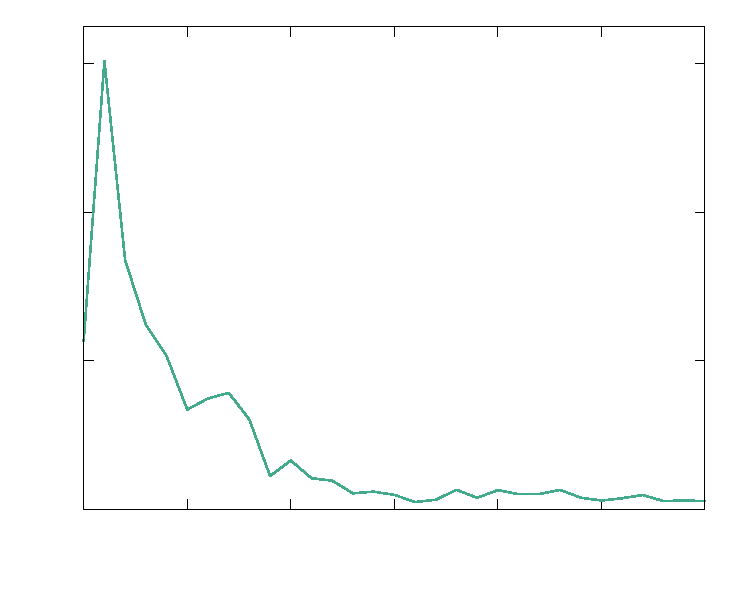
\includegraphics[width={354.00bp},height={283.00bp}]{./gnuplot/growth_a_01_coord_2}}%
    \gplfronttext
  \end{picture}%
\endgroup
}
    \resizebox{.45\textwidth}{!}{% GNUPLOT: LaTeX picture with Postscript
\begingroup
  \makeatletter
  \providecommand\color[2][]{%
    \GenericError{(gnuplot) \space\space\space\@spaces}{%
      Package color not loaded in conjunction with
      terminal option `colourtext'%
    }{See the gnuplot documentation for explanation.%
    }{Either use 'blacktext' in gnuplot or load the package
      color.sty in LaTeX.}%
    \renewcommand\color[2][]{}%
  }%
  \providecommand\includegraphics[2][]{%
    \GenericError{(gnuplot) \space\space\space\@spaces}{%
      Package graphicx or graphics not loaded%
    }{See the gnuplot documentation for explanation.%
    }{The gnuplot epslatex terminal needs graphicx.sty or graphics.sty.}%
    \renewcommand\includegraphics[2][]{}%
  }%
  \providecommand\rotatebox[2]{#2}%
  \@ifundefined{ifGPcolor}{%
    \newif\ifGPcolor
    \GPcolortrue
  }{}%
  \@ifundefined{ifGPblacktext}{%
    \newif\ifGPblacktext
    \GPblacktexttrue
  }{}%
  % define a \g@addto@macro without @ in the name:
  \let\gplgaddtomacro\g@addto@macro
  % define empty templates for all commands taking text:
  \gdef\gplbacktext{}%
  \gdef\gplfronttext{}%
  \makeatother
  \ifGPblacktext
    % no textcolor at all
    \def\colorrgb#1{}%
    \def\colorgray#1{}%
  \else
    % gray or color?
    \ifGPcolor
      \def\colorrgb#1{\color[rgb]{#1}}%
      \def\colorgray#1{\color[gray]{#1}}%
      \expandafter\def\csname LTw\endcsname{\color{white}}%
      \expandafter\def\csname LTb\endcsname{\color{black}}%
      \expandafter\def\csname LTa\endcsname{\color{black}}%
      \expandafter\def\csname LT0\endcsname{\color[rgb]{1,0,0}}%
      \expandafter\def\csname LT1\endcsname{\color[rgb]{0,1,0}}%
      \expandafter\def\csname LT2\endcsname{\color[rgb]{0,0,1}}%
      \expandafter\def\csname LT3\endcsname{\color[rgb]{1,0,1}}%
      \expandafter\def\csname LT4\endcsname{\color[rgb]{0,1,1}}%
      \expandafter\def\csname LT5\endcsname{\color[rgb]{1,1,0}}%
      \expandafter\def\csname LT6\endcsname{\color[rgb]{0,0,0}}%
      \expandafter\def\csname LT7\endcsname{\color[rgb]{1,0.3,0}}%
      \expandafter\def\csname LT8\endcsname{\color[rgb]{0.5,0.5,0.5}}%
    \else
      % gray
      \def\colorrgb#1{\color{black}}%
      \def\colorgray#1{\color[gray]{#1}}%
      \expandafter\def\csname LTw\endcsname{\color{white}}%
      \expandafter\def\csname LTb\endcsname{\color{black}}%
      \expandafter\def\csname LTa\endcsname{\color{black}}%
      \expandafter\def\csname LT0\endcsname{\color{black}}%
      \expandafter\def\csname LT1\endcsname{\color{black}}%
      \expandafter\def\csname LT2\endcsname{\color{black}}%
      \expandafter\def\csname LT3\endcsname{\color{black}}%
      \expandafter\def\csname LT4\endcsname{\color{black}}%
      \expandafter\def\csname LT5\endcsname{\color{black}}%
      \expandafter\def\csname LT6\endcsname{\color{black}}%
      \expandafter\def\csname LT7\endcsname{\color{black}}%
      \expandafter\def\csname LT8\endcsname{\color{black}}%
    \fi
  \fi
    \setlength{\unitlength}{0.0500bp}%
    \ifx\gptboxheight\undefined%
      \newlength{\gptboxheight}%
      \newlength{\gptboxwidth}%
      \newsavebox{\gptboxtext}%
    \fi%
    \setlength{\fboxrule}{0.5pt}%
    \setlength{\fboxsep}{1pt}%
    \definecolor{tbcol}{rgb}{1,1,1}%
\begin{picture}(7080.00,5660.00)%
    \gplgaddtomacro\gplbacktext{%
      \csname LTb\endcsname%%
      \put(692,767){\makebox(0,0)[r]{\strut{}$0.1$}}%
      \csname LTb\endcsname%%
      \put(692,1428){\makebox(0,0)[r]{\strut{}$0.2$}}%
      \csname LTb\endcsname%%
      \put(692,2090){\makebox(0,0)[r]{\strut{}$0.3$}}%
      \csname LTb\endcsname%%
      \put(692,2752){\makebox(0,0)[r]{\strut{}$0.4$}}%
      \csname LTb\endcsname%%
      \put(692,3414){\makebox(0,0)[r]{\strut{}$0.5$}}%
      \csname LTb\endcsname%%
      \put(692,4076){\makebox(0,0)[r]{\strut{}$0.6$}}%
      \csname LTb\endcsname%%
      \put(692,4738){\makebox(0,0)[r]{\strut{}$0.7$}}%
      \csname LTb\endcsname%%
      \put(692,5400){\makebox(0,0)[r]{\strut{}$0.8$}}%
      \csname LTb\endcsname%%
      \put(793,527){\makebox(0,0){\strut{}$1$}}%
      \csname LTb\endcsname%%
      \put(2284,527){\makebox(0,0){\strut{}$1.5$}}%
      \csname LTb\endcsname%%
      \put(3775,527){\makebox(0,0){\strut{}$2$}}%
      \csname LTb\endcsname%%
      \put(5266,527){\makebox(0,0){\strut{}$2.5$}}%
      \csname LTb\endcsname%%
      \put(6757,527){\makebox(0,0){\strut{}$3$}}%
    }%
    \gplgaddtomacro\gplfronttext{%
      \csname LTb\endcsname%%
      \put(195,3083){\rotatebox{-270}{\makebox(0,0){\strut{}$\psi_2$}}}%
      \csname LTb\endcsname%%
      \put(3775,167){\makebox(0,0){\strut{}$r$}}%
    }%
    \gplbacktext
    \put(0,0){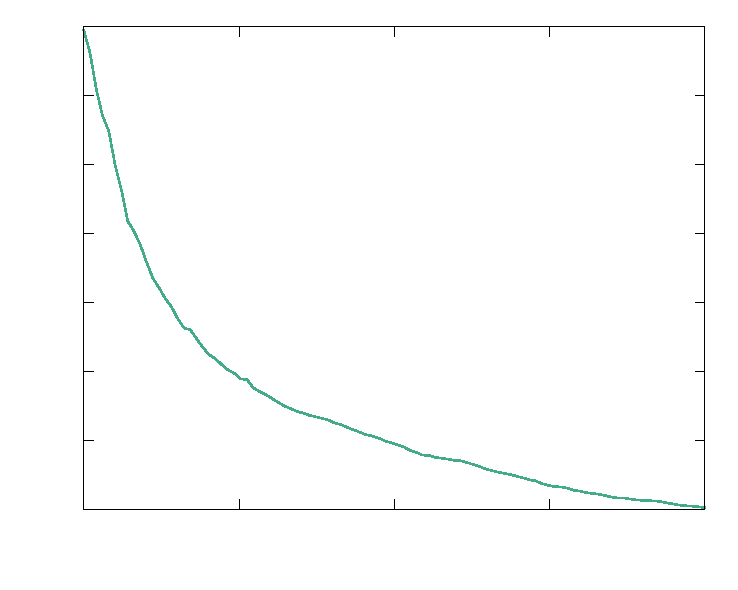
\includegraphics[width={354.00bp},height={283.00bp}]{./gnuplot/growth_a_01_correlation_1}}%
    \gplfronttext
  \end{picture}%
\endgroup
}
    \resizebox{.45\textwidth}{!}{% GNUPLOT: LaTeX picture with Postscript
\begingroup
  \makeatletter
  \providecommand\color[2][]{%
    \GenericError{(gnuplot) \space\space\space\@spaces}{%
      Package color not loaded in conjunction with
      terminal option `colourtext'%
    }{See the gnuplot documentation for explanation.%
    }{Either use 'blacktext' in gnuplot or load the package
      color.sty in LaTeX.}%
    \renewcommand\color[2][]{}%
  }%
  \providecommand\includegraphics[2][]{%
    \GenericError{(gnuplot) \space\space\space\@spaces}{%
      Package graphicx or graphics not loaded%
    }{See the gnuplot documentation for explanation.%
    }{The gnuplot epslatex terminal needs graphicx.sty or graphics.sty.}%
    \renewcommand\includegraphics[2][]{}%
  }%
  \providecommand\rotatebox[2]{#2}%
  \@ifundefined{ifGPcolor}{%
    \newif\ifGPcolor
    \GPcolortrue
  }{}%
  \@ifundefined{ifGPblacktext}{%
    \newif\ifGPblacktext
    \GPblacktexttrue
  }{}%
  % define a \g@addto@macro without @ in the name:
  \let\gplgaddtomacro\g@addto@macro
  % define empty templates for all commands taking text:
  \gdef\gplbacktext{}%
  \gdef\gplfronttext{}%
  \makeatother
  \ifGPblacktext
    % no textcolor at all
    \def\colorrgb#1{}%
    \def\colorgray#1{}%
  \else
    % gray or color?
    \ifGPcolor
      \def\colorrgb#1{\color[rgb]{#1}}%
      \def\colorgray#1{\color[gray]{#1}}%
      \expandafter\def\csname LTw\endcsname{\color{white}}%
      \expandafter\def\csname LTb\endcsname{\color{black}}%
      \expandafter\def\csname LTa\endcsname{\color{black}}%
      \expandafter\def\csname LT0\endcsname{\color[rgb]{1,0,0}}%
      \expandafter\def\csname LT1\endcsname{\color[rgb]{0,1,0}}%
      \expandafter\def\csname LT2\endcsname{\color[rgb]{0,0,1}}%
      \expandafter\def\csname LT3\endcsname{\color[rgb]{1,0,1}}%
      \expandafter\def\csname LT4\endcsname{\color[rgb]{0,1,1}}%
      \expandafter\def\csname LT5\endcsname{\color[rgb]{1,1,0}}%
      \expandafter\def\csname LT6\endcsname{\color[rgb]{0,0,0}}%
      \expandafter\def\csname LT7\endcsname{\color[rgb]{1,0.3,0}}%
      \expandafter\def\csname LT8\endcsname{\color[rgb]{0.5,0.5,0.5}}%
    \else
      % gray
      \def\colorrgb#1{\color{black}}%
      \def\colorgray#1{\color[gray]{#1}}%
      \expandafter\def\csname LTw\endcsname{\color{white}}%
      \expandafter\def\csname LTb\endcsname{\color{black}}%
      \expandafter\def\csname LTa\endcsname{\color{black}}%
      \expandafter\def\csname LT0\endcsname{\color{black}}%
      \expandafter\def\csname LT1\endcsname{\color{black}}%
      \expandafter\def\csname LT2\endcsname{\color{black}}%
      \expandafter\def\csname LT3\endcsname{\color{black}}%
      \expandafter\def\csname LT4\endcsname{\color{black}}%
      \expandafter\def\csname LT5\endcsname{\color{black}}%
      \expandafter\def\csname LT6\endcsname{\color{black}}%
      \expandafter\def\csname LT7\endcsname{\color{black}}%
      \expandafter\def\csname LT8\endcsname{\color{black}}%
    \fi
  \fi
    \setlength{\unitlength}{0.0500bp}%
    \ifx\gptboxheight\undefined%
      \newlength{\gptboxheight}%
      \newlength{\gptboxwidth}%
      \newsavebox{\gptboxtext}%
    \fi%
    \setlength{\fboxrule}{0.5pt}%
    \setlength{\fboxsep}{1pt}%
    \definecolor{tbcol}{rgb}{1,1,1}%
\begin{picture}(7080.00,5660.00)%
    \gplgaddtomacro\gplbacktext{%
      \csname LTb\endcsname%%
      \put(793,767){\makebox(0,0)[r]{\strut{}$0$}}%
      \csname LTb\endcsname%%
      \put(793,1428){\makebox(0,0)[r]{\strut{}$0.05$}}%
      \csname LTb\endcsname%%
      \put(793,2090){\makebox(0,0)[r]{\strut{}$0.1$}}%
      \csname LTb\endcsname%%
      \put(793,2752){\makebox(0,0)[r]{\strut{}$0.15$}}%
      \csname LTb\endcsname%%
      \put(793,3414){\makebox(0,0)[r]{\strut{}$0.2$}}%
      \csname LTb\endcsname%%
      \put(793,4076){\makebox(0,0)[r]{\strut{}$0.25$}}%
      \csname LTb\endcsname%%
      \put(793,4738){\makebox(0,0)[r]{\strut{}$0.3$}}%
      \csname LTb\endcsname%%
      \put(793,5400){\makebox(0,0)[r]{\strut{}$0.35$}}%
      \csname LTb\endcsname%%
      \put(894,527){\makebox(0,0){\strut{}$1$}}%
      \csname LTb\endcsname%%
      \put(2360,527){\makebox(0,0){\strut{}$1.5$}}%
      \csname LTb\endcsname%%
      \put(3826,527){\makebox(0,0){\strut{}$2$}}%
      \csname LTb\endcsname%%
      \put(5291,527){\makebox(0,0){\strut{}$2.5$}}%
      \csname LTb\endcsname%%
      \put(6757,527){\makebox(0,0){\strut{}$3$}}%
    }%
    \gplgaddtomacro\gplfronttext{%
      \csname LTb\endcsname%%
      \put(195,3083){\rotatebox{-270}{\makebox(0,0){\strut{}$\sigma_{\psi_2} / \psi_2$}}}%
      \csname LTb\endcsname%%
      \put(3826,167){\makebox(0,0){\strut{}$r$}}%
    }%
    \gplbacktext
    \put(0,0){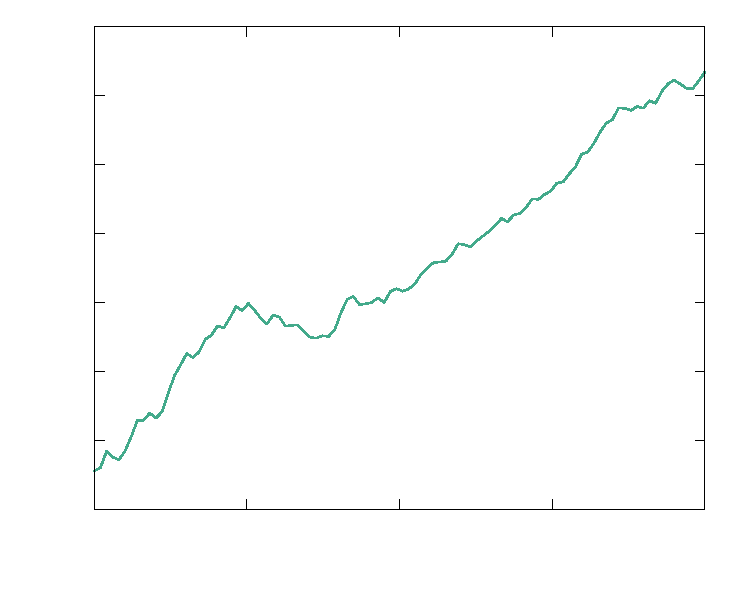
\includegraphics[width={354.00bp},height={283.00bp}]{./gnuplot/growth_a_01_correlation_2}}%
    \gplfronttext
  \end{picture}%
\endgroup
}
    \resizebox{.45\textwidth}{!}{% GNUPLOT: LaTeX picture with Postscript
\begingroup
  \makeatletter
  \providecommand\color[2][]{%
    \GenericError{(gnuplot) \space\space\space\@spaces}{%
      Package color not loaded in conjunction with
      terminal option `colourtext'%
    }{See the gnuplot documentation for explanation.%
    }{Either use 'blacktext' in gnuplot or load the package
      color.sty in LaTeX.}%
    \renewcommand\color[2][]{}%
  }%
  \providecommand\includegraphics[2][]{%
    \GenericError{(gnuplot) \space\space\space\@spaces}{%
      Package graphicx or graphics not loaded%
    }{See the gnuplot documentation for explanation.%
    }{The gnuplot epslatex terminal needs graphicx.sty or graphics.sty.}%
    \renewcommand\includegraphics[2][]{}%
  }%
  \providecommand\rotatebox[2]{#2}%
  \@ifundefined{ifGPcolor}{%
    \newif\ifGPcolor
    \GPcolortrue
  }{}%
  \@ifundefined{ifGPblacktext}{%
    \newif\ifGPblacktext
    \GPblacktexttrue
  }{}%
  % define a \g@addto@macro without @ in the name:
  \let\gplgaddtomacro\g@addto@macro
  % define empty templates for all commands taking text:
  \gdef\gplbacktext{}%
  \gdef\gplfronttext{}%
  \makeatother
  \ifGPblacktext
    % no textcolor at all
    \def\colorrgb#1{}%
    \def\colorgray#1{}%
  \else
    % gray or color?
    \ifGPcolor
      \def\colorrgb#1{\color[rgb]{#1}}%
      \def\colorgray#1{\color[gray]{#1}}%
      \expandafter\def\csname LTw\endcsname{\color{white}}%
      \expandafter\def\csname LTb\endcsname{\color{black}}%
      \expandafter\def\csname LTa\endcsname{\color{black}}%
      \expandafter\def\csname LT0\endcsname{\color[rgb]{1,0,0}}%
      \expandafter\def\csname LT1\endcsname{\color[rgb]{0,1,0}}%
      \expandafter\def\csname LT2\endcsname{\color[rgb]{0,0,1}}%
      \expandafter\def\csname LT3\endcsname{\color[rgb]{1,0,1}}%
      \expandafter\def\csname LT4\endcsname{\color[rgb]{0,1,1}}%
      \expandafter\def\csname LT5\endcsname{\color[rgb]{1,1,0}}%
      \expandafter\def\csname LT6\endcsname{\color[rgb]{0,0,0}}%
      \expandafter\def\csname LT7\endcsname{\color[rgb]{1,0.3,0}}%
      \expandafter\def\csname LT8\endcsname{\color[rgb]{0.5,0.5,0.5}}%
    \else
      % gray
      \def\colorrgb#1{\color{black}}%
      \def\colorgray#1{\color[gray]{#1}}%
      \expandafter\def\csname LTw\endcsname{\color{white}}%
      \expandafter\def\csname LTb\endcsname{\color{black}}%
      \expandafter\def\csname LTa\endcsname{\color{black}}%
      \expandafter\def\csname LT0\endcsname{\color{black}}%
      \expandafter\def\csname LT1\endcsname{\color{black}}%
      \expandafter\def\csname LT2\endcsname{\color{black}}%
      \expandafter\def\csname LT3\endcsname{\color{black}}%
      \expandafter\def\csname LT4\endcsname{\color{black}}%
      \expandafter\def\csname LT5\endcsname{\color{black}}%
      \expandafter\def\csname LT6\endcsname{\color{black}}%
      \expandafter\def\csname LT7\endcsname{\color{black}}%
      \expandafter\def\csname LT8\endcsname{\color{black}}%
    \fi
  \fi
    \setlength{\unitlength}{0.0500bp}%
    \ifx\gptboxheight\undefined%
      \newlength{\gptboxheight}%
      \newlength{\gptboxwidth}%
      \newsavebox{\gptboxtext}%
    \fi%
    \setlength{\fboxrule}{0.5pt}%
    \setlength{\fboxsep}{1pt}%
    \definecolor{tbcol}{rgb}{1,1,1}%
\begin{picture}(7080.00,5660.00)%
    \gplgaddtomacro\gplbacktext{%
      \csname LTb\endcsname%%
      \put(793,767){\makebox(0,0)[r]{\strut{}$0$}}%
      \csname LTb\endcsname%%
      \put(793,1925){\makebox(0,0)[r]{\strut{}$250$}}%
      \csname LTb\endcsname%%
      \put(793,3083){\makebox(0,0)[r]{\strut{}$500$}}%
      \csname LTb\endcsname%%
      \put(793,4241){\makebox(0,0)[r]{\strut{}$750$}}%
      \csname LTb\endcsname%%
      \put(793,5400){\makebox(0,0)[r]{\strut{}$1000$}}%
      \csname LTb\endcsname%%
      \put(894,527){\makebox(0,0){\strut{}$5$}}%
      \csname LTb\endcsname%%
      \put(1871,527){\makebox(0,0){\strut{}$5.5$}}%
      \csname LTb\endcsname%%
      \put(2848,527){\makebox(0,0){\strut{}$6$}}%
      \csname LTb\endcsname%%
      \put(3826,527){\makebox(0,0){\strut{}$6.5$}}%
      \csname LTb\endcsname%%
      \put(4803,527){\makebox(0,0){\strut{}$7$}}%
      \csname LTb\endcsname%%
      \put(5780,527){\makebox(0,0){\strut{}$7.5$}}%
      \csname LTb\endcsname%%
      \put(6757,527){\makebox(0,0){\strut{}$8$}}%
    }%
    \gplgaddtomacro\gplfronttext{%
      \csname LTb\endcsname%%
      \put(195,3083){\rotatebox{-270}{\makebox(0,0){\strut{}$N$}}}%
      \csname LTb\endcsname%%
      \put(3826,167){\makebox(0,0){\strut{}$a$}}%
      \csname LTb\endcsname%%
      \put(1342,4920){\makebox(0,0)[l]{\strut{}Sprejete rotacije}}%
      \csname LTb\endcsname%%
      \put(1342,5160){\makebox(0,0)[l]{\strut{}Zavrnjene rotacije}}%
    }%
    \gplbacktext
    \put(0,0){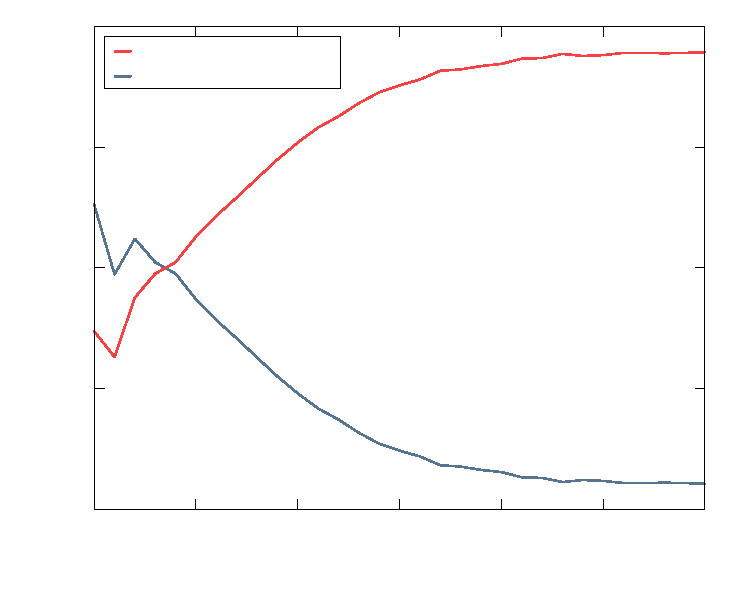
\includegraphics[width={354.00bp},height={283.00bp}]{./gnuplot/growth_a_01_rotations_1}}%
    \gplfronttext
  \end{picture}%
\endgroup
}
    \resizebox{.45\textwidth}{!}{% GNUPLOT: LaTeX picture with Postscript
\begingroup
  \makeatletter
  \providecommand\color[2][]{%
    \GenericError{(gnuplot) \space\space\space\@spaces}{%
      Package color not loaded in conjunction with
      terminal option `colourtext'%
    }{See the gnuplot documentation for explanation.%
    }{Either use 'blacktext' in gnuplot or load the package
      color.sty in LaTeX.}%
    \renewcommand\color[2][]{}%
  }%
  \providecommand\includegraphics[2][]{%
    \GenericError{(gnuplot) \space\space\space\@spaces}{%
      Package graphicx or graphics not loaded%
    }{See the gnuplot documentation for explanation.%
    }{The gnuplot epslatex terminal needs graphicx.sty or graphics.sty.}%
    \renewcommand\includegraphics[2][]{}%
  }%
  \providecommand\rotatebox[2]{#2}%
  \@ifundefined{ifGPcolor}{%
    \newif\ifGPcolor
    \GPcolortrue
  }{}%
  \@ifundefined{ifGPblacktext}{%
    \newif\ifGPblacktext
    \GPblacktexttrue
  }{}%
  % define a \g@addto@macro without @ in the name:
  \let\gplgaddtomacro\g@addto@macro
  % define empty templates for all commands taking text:
  \gdef\gplbacktext{}%
  \gdef\gplfronttext{}%
  \makeatother
  \ifGPblacktext
    % no textcolor at all
    \def\colorrgb#1{}%
    \def\colorgray#1{}%
  \else
    % gray or color?
    \ifGPcolor
      \def\colorrgb#1{\color[rgb]{#1}}%
      \def\colorgray#1{\color[gray]{#1}}%
      \expandafter\def\csname LTw\endcsname{\color{white}}%
      \expandafter\def\csname LTb\endcsname{\color{black}}%
      \expandafter\def\csname LTa\endcsname{\color{black}}%
      \expandafter\def\csname LT0\endcsname{\color[rgb]{1,0,0}}%
      \expandafter\def\csname LT1\endcsname{\color[rgb]{0,1,0}}%
      \expandafter\def\csname LT2\endcsname{\color[rgb]{0,0,1}}%
      \expandafter\def\csname LT3\endcsname{\color[rgb]{1,0,1}}%
      \expandafter\def\csname LT4\endcsname{\color[rgb]{0,1,1}}%
      \expandafter\def\csname LT5\endcsname{\color[rgb]{1,1,0}}%
      \expandafter\def\csname LT6\endcsname{\color[rgb]{0,0,0}}%
      \expandafter\def\csname LT7\endcsname{\color[rgb]{1,0.3,0}}%
      \expandafter\def\csname LT8\endcsname{\color[rgb]{0.5,0.5,0.5}}%
    \else
      % gray
      \def\colorrgb#1{\color{black}}%
      \def\colorgray#1{\color[gray]{#1}}%
      \expandafter\def\csname LTw\endcsname{\color{white}}%
      \expandafter\def\csname LTb\endcsname{\color{black}}%
      \expandafter\def\csname LTa\endcsname{\color{black}}%
      \expandafter\def\csname LT0\endcsname{\color{black}}%
      \expandafter\def\csname LT1\endcsname{\color{black}}%
      \expandafter\def\csname LT2\endcsname{\color{black}}%
      \expandafter\def\csname LT3\endcsname{\color{black}}%
      \expandafter\def\csname LT4\endcsname{\color{black}}%
      \expandafter\def\csname LT5\endcsname{\color{black}}%
      \expandafter\def\csname LT6\endcsname{\color{black}}%
      \expandafter\def\csname LT7\endcsname{\color{black}}%
      \expandafter\def\csname LT8\endcsname{\color{black}}%
    \fi
  \fi
    \setlength{\unitlength}{0.0500bp}%
    \ifx\gptboxheight\undefined%
      \newlength{\gptboxheight}%
      \newlength{\gptboxwidth}%
      \newsavebox{\gptboxtext}%
    \fi%
    \setlength{\fboxrule}{0.5pt}%
    \setlength{\fboxsep}{1pt}%
    \definecolor{tbcol}{rgb}{1,1,1}%
\begin{picture}(7080.00,5660.00)%
    \gplgaddtomacro\gplbacktext{%
      \csname LTb\endcsname%%
      \put(692,767){\makebox(0,0)[r]{\strut{}$0$}}%
      \csname LTb\endcsname%%
      \put(692,2311){\makebox(0,0)[r]{\strut{}$0.1$}}%
      \csname LTb\endcsname%%
      \put(692,3855){\makebox(0,0)[r]{\strut{}$0.2$}}%
      \csname LTb\endcsname%%
      \put(692,5400){\makebox(0,0)[r]{\strut{}$0.3$}}%
      \csname LTb\endcsname%%
      \put(793,527){\makebox(0,0){\strut{}$5$}}%
      \csname LTb\endcsname%%
      \put(1787,527){\makebox(0,0){\strut{}$5.5$}}%
      \csname LTb\endcsname%%
      \put(2781,527){\makebox(0,0){\strut{}$6$}}%
      \csname LTb\endcsname%%
      \put(3775,527){\makebox(0,0){\strut{}$6.5$}}%
      \csname LTb\endcsname%%
      \put(4769,527){\makebox(0,0){\strut{}$7$}}%
      \csname LTb\endcsname%%
      \put(5763,527){\makebox(0,0){\strut{}$7.5$}}%
      \csname LTb\endcsname%%
      \put(6757,527){\makebox(0,0){\strut{}$8$}}%
    }%
    \gplgaddtomacro\gplfronttext{%
      \csname LTb\endcsname%%
      \put(195,3083){\rotatebox{-270}{\makebox(0,0){\strut{}$\sigma_N / N$}}}%
      \csname LTb\endcsname%%
      \put(3775,167){\makebox(0,0){\strut{}$a$}}%
      \csname LTb\endcsname%%
      \put(4743,4920){\makebox(0,0)[l]{\strut{}Sprejete rotacije}}%
      \csname LTb\endcsname%%
      \put(4743,5160){\makebox(0,0)[l]{\strut{}Zavrnjene rotacije}}%
    }%
    \gplbacktext
    \put(0,0){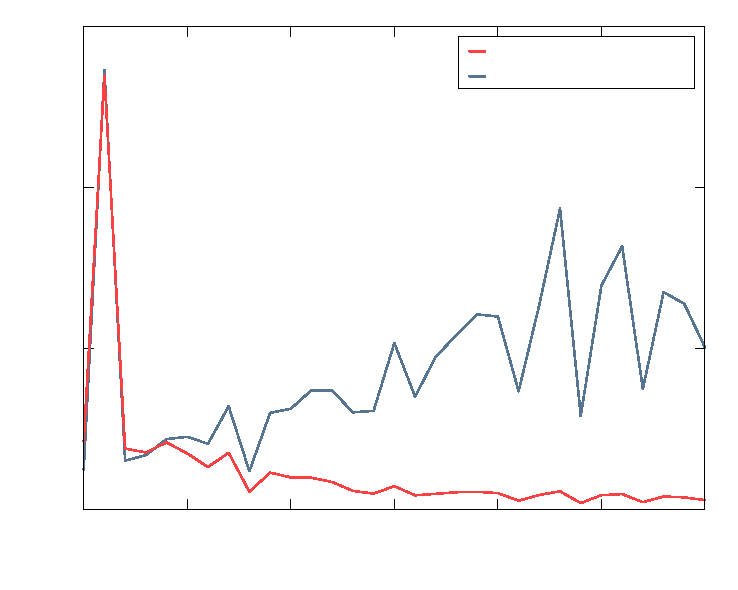
\includegraphics[width={354.00bp},height={283.00bp}]{./gnuplot/growth_a_01_rotations_2}}%
    \gplfronttext
  \end{picture}%
\endgroup
}
    \caption{Spreminjanje energije, povprečnega števila kontaktov s~sosednjimi elipsami,
    korelacijske orientacijske funkcije in števila sprejetih ter zavrnjenih rotacij tekom
    relaksacije sistema. Povprečeno po desetih poskusih relaksacije.}
    \label{fig:average_a_01}
\end{figure}